\documentclass{book}

\usepackage{amssymb}
\usepackage{amsfonts}
\usepackage{amsmath}
\usepackage{graphicx}
\usepackage{units}
\usepackage{hyperref}
\usepackage{listings}
\usepackage{pythonhighlight}
%\usepackage{authblk}

\graphicspath {{Figures/}}

 %%%%%%%%%%%%%%%%%%%%%%%%%%%%%%%%%%%%%%%%%%%%%%%%%%%%%%%%%%%%%%%%%%%%%%%%%%%%%%%% 
%%% ~ Arduino Language - Arduino IDE Colors ~                                  %%%
%%%                                                                            %%%
%%% Kyle Rocha-Brownell | 10/2/2017 | No Licence                               %%%
%%% -------------------------------------------------------------------------- %%%
%%%                                                                            %%%
%%% Place this file in your working directory (next to the latex file you're   %%%
%%% working on).  To add it to your project, place:                            %%%
%%%     %%%%%%%%%%%%%%%%%%%%%%%%%%%%%%%%%%%%%%%%%%%%%%%%%%%%%%%%%%%%%%%%%%%%%%%%%%%%%%%% 
%%% ~ Arduino Language - Arduino IDE Colors ~                                  %%%
%%%                                                                            %%%
%%% Kyle Rocha-Brownell | 10/2/2017 | No Licence                               %%%
%%% -------------------------------------------------------------------------- %%%
%%%                                                                            %%%
%%% Place this file in your working directory (next to the latex file you're   %%%
%%% working on).  To add it to your project, place:                            %%%
%%%     %%%%%%%%%%%%%%%%%%%%%%%%%%%%%%%%%%%%%%%%%%%%%%%%%%%%%%%%%%%%%%%%%%%%%%%%%%%%%%%% 
%%% ~ Arduino Language - Arduino IDE Colors ~                                  %%%
%%%                                                                            %%%
%%% Kyle Rocha-Brownell | 10/2/2017 | No Licence                               %%%
%%% -------------------------------------------------------------------------- %%%
%%%                                                                            %%%
%%% Place this file in your working directory (next to the latex file you're   %%%
%%% working on).  To add it to your project, place:                            %%%
%%%    \input{arduinoLanguage.tex}                                             %%%
%%% somewhere before \begin{document} in your latex file.                      %%%
%%%                                                                            %%%
%%% In your document, place your arduino code between:                         %%%
%%%   \begin{lstlisting}[language=Arduino]                                     %%%
%%% and:                                                                       %%%
%%%   \end{lstlisting}                                                         %%%
%%%                                                                            %%%
%%% Or create your own style to add non-built-in functions and variables.      %%%
%%%                                                                            %%%
 %%%%%%%%%%%%%%%%%%%%%%%%%%%%%%%%%%%%%%%%%%%%%%%%%%%%%%%%%%%%%%%%%%%%%%%%%%%%%%%% 

\usepackage{color}
\usepackage{listings}    
\usepackage{courier}

%%% Define Custom IDE Colors %%%
\definecolor{arduinoGreen}    {rgb} {0.17, 0.43, 0.01}
\definecolor{arduinoGrey}     {rgb} {0.47, 0.47, 0.33}
\definecolor{arduinoOrange}   {rgb} {0.8 , 0.4 , 0   }
\definecolor{arduinoBlue}     {rgb} {0.01, 0.61, 0.98}
\definecolor{arduinoDarkBlue} {rgb} {0.0 , 0.2 , 0.5 }

%%% Define Arduino Language %%%
\lstdefinelanguage{Arduino}{
  language=C++, % begin with default C++ settings 
%
%
  %%% Keyword Color Group 1 %%%  (called KEYWORD3 by arduino)
  keywordstyle=\color{arduinoGreen},   
  deletekeywords={  % remove all arduino keywords that might be in c++
                break, case, override, final, continue, default, do, else, for, 
                if, return, goto, switch, throw, try, while, setup, loop, export, 
                not, or, and, xor, include, define, elif, else, error, if, ifdef, 
                ifndef, pragma, warning,
                HIGH, LOW, INPUT, INPUT_PULLUP, OUTPUT, DEC, BIN, HEX, OCT, PI, 
                HALF_PI, TWO_PI, LSBFIRST, MSBFIRST, CHANGE, FALLING, RISING, 
                DEFAULT, EXTERNAL, INTERNAL, INTERNAL1V1, INTERNAL2V56, LED_BUILTIN, 
                LED_BUILTIN_RX, LED_BUILTIN_TX, DIGITAL_MESSAGE, FIRMATA_STRING, 
                ANALOG_MESSAGE, REPORT_DIGITAL, REPORT_ANALOG, SET_PIN_MODE, 
                SYSTEM_RESET, SYSEX_START, auto, int8_t, int16_t, int32_t, int64_t, 
                uint8_t, uint16_t, uint32_t, uint64_t, char16_t, char32_t, operator, 
                enum, delete, bool, boolean, byte, char, const, false, float, double, 
                null, NULL, int, long, new, private, protected, public, short, 
                signed, static, volatile, String, void, true, unsigned, word, array, 
                sizeof, dynamic_cast, typedef, const_cast, struct, static_cast, union, 
                friend, extern, class, reinterpret_cast, register, explicit, inline, 
                _Bool, complex, _Complex, _Imaginary, atomic_bool, atomic_char, 
                atomic_schar, atomic_uchar, atomic_short, atomic_ushort, atomic_int, 
                atomic_uint, atomic_long, atomic_ulong, atomic_llong, atomic_ullong, 
                virtual, PROGMEM,
                Serial, Serial1, Serial2, Serial3, SerialUSB, Keyboard, Mouse,
                abs, acos, asin, atan, atan2, ceil, constrain, cos, degrees, exp, 
                floor, log, map, max, min, radians, random, randomSeed, round, sin, 
                sq, sqrt, tan, pow, bitRead, bitWrite, bitSet, bitClear, bit, 
                highByte, lowByte, analogReference, analogRead, 
                analogReadResolution, analogWrite, analogWriteResolution, 
                attachInterrupt, detachInterrupt, digitalPinToInterrupt, delay, 
                delayMicroseconds, digitalWrite, digitalRead, interrupts, millis, 
                micros, noInterrupts, noTone, pinMode, pulseIn, pulseInLong, shiftIn, 
                shiftOut, tone, yield, Stream, begin, end, peek, read, print, 
                println, available, availableForWrite, flush, setTimeout, find, 
                findUntil, parseInt, parseFloat, readBytes, readBytesUntil, readString, 
                readStringUntil, trim, toUpperCase, toLowerCase, charAt, compareTo, 
                concat, endsWith, startsWith, equals, equalsIgnoreCase, getBytes, 
                indexOf, lastIndexOf, length, replace, setCharAt, substring, 
                toCharArray, toInt, press, release, releaseAll, accept, click, move, 
                isPressed, isAlphaNumeric, isAlpha, isAscii, isWhitespace, isControl, 
                isDigit, isGraph, isLowerCase, isPrintable, isPunct, isSpace, 
                isUpperCase, isHexadecimalDigit, 
                }, 
  morekeywords={   % add arduino structures to group 1
                break, case, override, final, continue, default, do, else, for, 
                if, return, goto, switch, throw, try, while, setup, loop, export, 
                not, or, and, xor, include, define, elif, else, error, if, ifdef, 
                ifndef, pragma, warning,
                }, 
% 
%
  %%% Keyword Color Group 2 %%%  (called LITERAL1 by arduino)
  keywordstyle=[2]\color{arduinoBlue},   
  keywords=[2]{   % add variables and dataTypes as 2nd group  
                HIGH, LOW, INPUT, INPUT_PULLUP, OUTPUT, DEC, BIN, HEX, OCT, PI, 
                HALF_PI, TWO_PI, LSBFIRST, MSBFIRST, CHANGE, FALLING, RISING, 
                DEFAULT, EXTERNAL, INTERNAL, INTERNAL1V1, INTERNAL2V56, LED_BUILTIN, 
                LED_BUILTIN_RX, LED_BUILTIN_TX, DIGITAL_MESSAGE, FIRMATA_STRING, 
                ANALOG_MESSAGE, REPORT_DIGITAL, REPORT_ANALOG, SET_PIN_MODE, 
                SYSTEM_RESET, SYSEX_START, auto, int8_t, int16_t, int32_t, int64_t, 
                uint8_t, uint16_t, uint32_t, uint64_t, char16_t, char32_t, operator, 
                enum, delete, bool, boolean, byte, char, const, false, float, double, 
                null, NULL, int, long, new, private, protected, public, short, 
                signed, static, volatile, String, void, true, unsigned, word, array, 
                sizeof, dynamic_cast, typedef, const_cast, struct, static_cast, union, 
                friend, extern, class, reinterpret_cast, register, explicit, inline, 
                _Bool, complex, _Complex, _Imaginary, atomic_bool, atomic_char, 
                atomic_schar, atomic_uchar, atomic_short, atomic_ushort, atomic_int, 
                atomic_uint, atomic_long, atomic_ulong, atomic_llong, atomic_ullong, 
                virtual, PROGMEM,
                },  
% 
%
  %%% Keyword Color Group 3 %%%  (called KEYWORD1 by arduino)
  keywordstyle=[3]\bfseries\color{arduinoOrange},
  keywords=[3]{  % add built-in functions as a 3rd group
                Serial, Serial1, Serial2, Serial3, SerialUSB, Keyboard, Mouse,
                },      
%
%
  %%% Keyword Color Group 4 %%%  (called KEYWORD2 by arduino)
  keywordstyle=[4]\color{arduinoOrange},
  keywords=[4]{  % add more built-in functions as a 4th group
                abs, acos, asin, atan, atan2, ceil, constrain, cos, degrees, exp, 
                floor, log, map, max, min, radians, random, randomSeed, round, sin, 
                sq, sqrt, tan, pow, bitRead, bitWrite, bitSet, bitClear, bit, 
                highByte, lowByte, analogReference, analogRead, 
                analogReadResolution, analogWrite, analogWriteResolution, 
                attachInterrupt, detachInterrupt, digitalPinToInterrupt, delay, 
                delayMicroseconds, digitalWrite, digitalRead, interrupts, millis, 
                micros, noInterrupts, noTone, pinMode, pulseIn, pulseInLong, shiftIn, 
                shiftOut, tone, yield, Stream, begin, end, peek, read, print, 
                println, available, availableForWrite, flush, setTimeout, find, 
                findUntil, parseInt, parseFloat, readBytes, readBytesUntil, readString, 
                readStringUntil, trim, toUpperCase, toLowerCase, charAt, compareTo, 
                concat, endsWith, startsWith, equals, equalsIgnoreCase, getBytes, 
                indexOf, lastIndexOf, length, replace, setCharAt, substring, 
                toCharArray, toInt, press, release, releaseAll, accept, click, move, 
                isPressed, isAlphaNumeric, isAlpha, isAscii, isWhitespace, isControl, 
                isDigit, isGraph, isLowerCase, isPrintable, isPunct, isSpace, 
                isUpperCase, isHexadecimalDigit, 
                },      
%
%
  %%% Set Other Colors %%%
  stringstyle=\color{arduinoDarkBlue},    
  commentstyle=\color{arduinoGrey},    
%          
%   
  %%%% Line Numbering %%%%
%  numbers=left,                    
%  numbersep=5pt,                   
%  numberstyle=\color{arduinoGrey},    
  %stepnumber=2,                      % show every 2 line numbers
%
%
  frame=single, 	% Adds a boxed frame around the code
  %%%% Code Box Style %%%%
  breaklines=false,%true,                    % wordwrapping
  tabsize=2,         
  basicstyle=\ttfamily
}
                                             %%%
%%% somewhere before \begin{document} in your latex file.                      %%%
%%%                                                                            %%%
%%% In your document, place your arduino code between:                         %%%
%%%   \begin{lstlisting}[language=Arduino]                                     %%%
%%% and:                                                                       %%%
%%%   \end{lstlisting}                                                         %%%
%%%                                                                            %%%
%%% Or create your own style to add non-built-in functions and variables.      %%%
%%%                                                                            %%%
 %%%%%%%%%%%%%%%%%%%%%%%%%%%%%%%%%%%%%%%%%%%%%%%%%%%%%%%%%%%%%%%%%%%%%%%%%%%%%%%% 

\usepackage{color}
\usepackage{listings}    
\usepackage{courier}

%%% Define Custom IDE Colors %%%
\definecolor{arduinoGreen}    {rgb} {0.17, 0.43, 0.01}
\definecolor{arduinoGrey}     {rgb} {0.47, 0.47, 0.33}
\definecolor{arduinoOrange}   {rgb} {0.8 , 0.4 , 0   }
\definecolor{arduinoBlue}     {rgb} {0.01, 0.61, 0.98}
\definecolor{arduinoDarkBlue} {rgb} {0.0 , 0.2 , 0.5 }

%%% Define Arduino Language %%%
\lstdefinelanguage{Arduino}{
  language=C++, % begin with default C++ settings 
%
%
  %%% Keyword Color Group 1 %%%  (called KEYWORD3 by arduino)
  keywordstyle=\color{arduinoGreen},   
  deletekeywords={  % remove all arduino keywords that might be in c++
                break, case, override, final, continue, default, do, else, for, 
                if, return, goto, switch, throw, try, while, setup, loop, export, 
                not, or, and, xor, include, define, elif, else, error, if, ifdef, 
                ifndef, pragma, warning,
                HIGH, LOW, INPUT, INPUT_PULLUP, OUTPUT, DEC, BIN, HEX, OCT, PI, 
                HALF_PI, TWO_PI, LSBFIRST, MSBFIRST, CHANGE, FALLING, RISING, 
                DEFAULT, EXTERNAL, INTERNAL, INTERNAL1V1, INTERNAL2V56, LED_BUILTIN, 
                LED_BUILTIN_RX, LED_BUILTIN_TX, DIGITAL_MESSAGE, FIRMATA_STRING, 
                ANALOG_MESSAGE, REPORT_DIGITAL, REPORT_ANALOG, SET_PIN_MODE, 
                SYSTEM_RESET, SYSEX_START, auto, int8_t, int16_t, int32_t, int64_t, 
                uint8_t, uint16_t, uint32_t, uint64_t, char16_t, char32_t, operator, 
                enum, delete, bool, boolean, byte, char, const, false, float, double, 
                null, NULL, int, long, new, private, protected, public, short, 
                signed, static, volatile, String, void, true, unsigned, word, array, 
                sizeof, dynamic_cast, typedef, const_cast, struct, static_cast, union, 
                friend, extern, class, reinterpret_cast, register, explicit, inline, 
                _Bool, complex, _Complex, _Imaginary, atomic_bool, atomic_char, 
                atomic_schar, atomic_uchar, atomic_short, atomic_ushort, atomic_int, 
                atomic_uint, atomic_long, atomic_ulong, atomic_llong, atomic_ullong, 
                virtual, PROGMEM,
                Serial, Serial1, Serial2, Serial3, SerialUSB, Keyboard, Mouse,
                abs, acos, asin, atan, atan2, ceil, constrain, cos, degrees, exp, 
                floor, log, map, max, min, radians, random, randomSeed, round, sin, 
                sq, sqrt, tan, pow, bitRead, bitWrite, bitSet, bitClear, bit, 
                highByte, lowByte, analogReference, analogRead, 
                analogReadResolution, analogWrite, analogWriteResolution, 
                attachInterrupt, detachInterrupt, digitalPinToInterrupt, delay, 
                delayMicroseconds, digitalWrite, digitalRead, interrupts, millis, 
                micros, noInterrupts, noTone, pinMode, pulseIn, pulseInLong, shiftIn, 
                shiftOut, tone, yield, Stream, begin, end, peek, read, print, 
                println, available, availableForWrite, flush, setTimeout, find, 
                findUntil, parseInt, parseFloat, readBytes, readBytesUntil, readString, 
                readStringUntil, trim, toUpperCase, toLowerCase, charAt, compareTo, 
                concat, endsWith, startsWith, equals, equalsIgnoreCase, getBytes, 
                indexOf, lastIndexOf, length, replace, setCharAt, substring, 
                toCharArray, toInt, press, release, releaseAll, accept, click, move, 
                isPressed, isAlphaNumeric, isAlpha, isAscii, isWhitespace, isControl, 
                isDigit, isGraph, isLowerCase, isPrintable, isPunct, isSpace, 
                isUpperCase, isHexadecimalDigit, 
                }, 
  morekeywords={   % add arduino structures to group 1
                break, case, override, final, continue, default, do, else, for, 
                if, return, goto, switch, throw, try, while, setup, loop, export, 
                not, or, and, xor, include, define, elif, else, error, if, ifdef, 
                ifndef, pragma, warning,
                }, 
% 
%
  %%% Keyword Color Group 2 %%%  (called LITERAL1 by arduino)
  keywordstyle=[2]\color{arduinoBlue},   
  keywords=[2]{   % add variables and dataTypes as 2nd group  
                HIGH, LOW, INPUT, INPUT_PULLUP, OUTPUT, DEC, BIN, HEX, OCT, PI, 
                HALF_PI, TWO_PI, LSBFIRST, MSBFIRST, CHANGE, FALLING, RISING, 
                DEFAULT, EXTERNAL, INTERNAL, INTERNAL1V1, INTERNAL2V56, LED_BUILTIN, 
                LED_BUILTIN_RX, LED_BUILTIN_TX, DIGITAL_MESSAGE, FIRMATA_STRING, 
                ANALOG_MESSAGE, REPORT_DIGITAL, REPORT_ANALOG, SET_PIN_MODE, 
                SYSTEM_RESET, SYSEX_START, auto, int8_t, int16_t, int32_t, int64_t, 
                uint8_t, uint16_t, uint32_t, uint64_t, char16_t, char32_t, operator, 
                enum, delete, bool, boolean, byte, char, const, false, float, double, 
                null, NULL, int, long, new, private, protected, public, short, 
                signed, static, volatile, String, void, true, unsigned, word, array, 
                sizeof, dynamic_cast, typedef, const_cast, struct, static_cast, union, 
                friend, extern, class, reinterpret_cast, register, explicit, inline, 
                _Bool, complex, _Complex, _Imaginary, atomic_bool, atomic_char, 
                atomic_schar, atomic_uchar, atomic_short, atomic_ushort, atomic_int, 
                atomic_uint, atomic_long, atomic_ulong, atomic_llong, atomic_ullong, 
                virtual, PROGMEM,
                },  
% 
%
  %%% Keyword Color Group 3 %%%  (called KEYWORD1 by arduino)
  keywordstyle=[3]\bfseries\color{arduinoOrange},
  keywords=[3]{  % add built-in functions as a 3rd group
                Serial, Serial1, Serial2, Serial3, SerialUSB, Keyboard, Mouse,
                },      
%
%
  %%% Keyword Color Group 4 %%%  (called KEYWORD2 by arduino)
  keywordstyle=[4]\color{arduinoOrange},
  keywords=[4]{  % add more built-in functions as a 4th group
                abs, acos, asin, atan, atan2, ceil, constrain, cos, degrees, exp, 
                floor, log, map, max, min, radians, random, randomSeed, round, sin, 
                sq, sqrt, tan, pow, bitRead, bitWrite, bitSet, bitClear, bit, 
                highByte, lowByte, analogReference, analogRead, 
                analogReadResolution, analogWrite, analogWriteResolution, 
                attachInterrupt, detachInterrupt, digitalPinToInterrupt, delay, 
                delayMicroseconds, digitalWrite, digitalRead, interrupts, millis, 
                micros, noInterrupts, noTone, pinMode, pulseIn, pulseInLong, shiftIn, 
                shiftOut, tone, yield, Stream, begin, end, peek, read, print, 
                println, available, availableForWrite, flush, setTimeout, find, 
                findUntil, parseInt, parseFloat, readBytes, readBytesUntil, readString, 
                readStringUntil, trim, toUpperCase, toLowerCase, charAt, compareTo, 
                concat, endsWith, startsWith, equals, equalsIgnoreCase, getBytes, 
                indexOf, lastIndexOf, length, replace, setCharAt, substring, 
                toCharArray, toInt, press, release, releaseAll, accept, click, move, 
                isPressed, isAlphaNumeric, isAlpha, isAscii, isWhitespace, isControl, 
                isDigit, isGraph, isLowerCase, isPrintable, isPunct, isSpace, 
                isUpperCase, isHexadecimalDigit, 
                },      
%
%
  %%% Set Other Colors %%%
  stringstyle=\color{arduinoDarkBlue},    
  commentstyle=\color{arduinoGrey},    
%          
%   
  %%%% Line Numbering %%%%
%  numbers=left,                    
%  numbersep=5pt,                   
%  numberstyle=\color{arduinoGrey},    
  %stepnumber=2,                      % show every 2 line numbers
%
%
  frame=single, 	% Adds a boxed frame around the code
  %%%% Code Box Style %%%%
  breaklines=false,%true,                    % wordwrapping
  tabsize=2,         
  basicstyle=\ttfamily
}
                                             %%%
%%% somewhere before \begin{document} in your latex file.                      %%%
%%%                                                                            %%%
%%% In your document, place your arduino code between:                         %%%
%%%   \begin{lstlisting}[language=Arduino]                                     %%%
%%% and:                                                                       %%%
%%%   \end{lstlisting}                                                         %%%
%%%                                                                            %%%
%%% Or create your own style to add non-built-in functions and variables.      %%%
%%%                                                                            %%%
 %%%%%%%%%%%%%%%%%%%%%%%%%%%%%%%%%%%%%%%%%%%%%%%%%%%%%%%%%%%%%%%%%%%%%%%%%%%%%%%% 

\usepackage{color}
\usepackage{listings}    
\usepackage{courier}

%%% Define Custom IDE Colors %%%
\definecolor{arduinoGreen}    {rgb} {0.17, 0.43, 0.01}
\definecolor{arduinoGrey}     {rgb} {0.47, 0.47, 0.33}
\definecolor{arduinoOrange}   {rgb} {0.8 , 0.4 , 0   }
\definecolor{arduinoBlue}     {rgb} {0.01, 0.61, 0.98}
\definecolor{arduinoDarkBlue} {rgb} {0.0 , 0.2 , 0.5 }

%%% Define Arduino Language %%%
\lstdefinelanguage{Arduino}{
  language=C++, % begin with default C++ settings 
%
%
  %%% Keyword Color Group 1 %%%  (called KEYWORD3 by arduino)
  keywordstyle=\color{arduinoGreen},   
  deletekeywords={  % remove all arduino keywords that might be in c++
                break, case, override, final, continue, default, do, else, for, 
                if, return, goto, switch, throw, try, while, setup, loop, export, 
                not, or, and, xor, include, define, elif, else, error, if, ifdef, 
                ifndef, pragma, warning,
                HIGH, LOW, INPUT, INPUT_PULLUP, OUTPUT, DEC, BIN, HEX, OCT, PI, 
                HALF_PI, TWO_PI, LSBFIRST, MSBFIRST, CHANGE, FALLING, RISING, 
                DEFAULT, EXTERNAL, INTERNAL, INTERNAL1V1, INTERNAL2V56, LED_BUILTIN, 
                LED_BUILTIN_RX, LED_BUILTIN_TX, DIGITAL_MESSAGE, FIRMATA_STRING, 
                ANALOG_MESSAGE, REPORT_DIGITAL, REPORT_ANALOG, SET_PIN_MODE, 
                SYSTEM_RESET, SYSEX_START, auto, int8_t, int16_t, int32_t, int64_t, 
                uint8_t, uint16_t, uint32_t, uint64_t, char16_t, char32_t, operator, 
                enum, delete, bool, boolean, byte, char, const, false, float, double, 
                null, NULL, int, long, new, private, protected, public, short, 
                signed, static, volatile, String, void, true, unsigned, word, array, 
                sizeof, dynamic_cast, typedef, const_cast, struct, static_cast, union, 
                friend, extern, class, reinterpret_cast, register, explicit, inline, 
                _Bool, complex, _Complex, _Imaginary, atomic_bool, atomic_char, 
                atomic_schar, atomic_uchar, atomic_short, atomic_ushort, atomic_int, 
                atomic_uint, atomic_long, atomic_ulong, atomic_llong, atomic_ullong, 
                virtual, PROGMEM,
                Serial, Serial1, Serial2, Serial3, SerialUSB, Keyboard, Mouse,
                abs, acos, asin, atan, atan2, ceil, constrain, cos, degrees, exp, 
                floor, log, map, max, min, radians, random, randomSeed, round, sin, 
                sq, sqrt, tan, pow, bitRead, bitWrite, bitSet, bitClear, bit, 
                highByte, lowByte, analogReference, analogRead, 
                analogReadResolution, analogWrite, analogWriteResolution, 
                attachInterrupt, detachInterrupt, digitalPinToInterrupt, delay, 
                delayMicroseconds, digitalWrite, digitalRead, interrupts, millis, 
                micros, noInterrupts, noTone, pinMode, pulseIn, pulseInLong, shiftIn, 
                shiftOut, tone, yield, Stream, begin, end, peek, read, print, 
                println, available, availableForWrite, flush, setTimeout, find, 
                findUntil, parseInt, parseFloat, readBytes, readBytesUntil, readString, 
                readStringUntil, trim, toUpperCase, toLowerCase, charAt, compareTo, 
                concat, endsWith, startsWith, equals, equalsIgnoreCase, getBytes, 
                indexOf, lastIndexOf, length, replace, setCharAt, substring, 
                toCharArray, toInt, press, release, releaseAll, accept, click, move, 
                isPressed, isAlphaNumeric, isAlpha, isAscii, isWhitespace, isControl, 
                isDigit, isGraph, isLowerCase, isPrintable, isPunct, isSpace, 
                isUpperCase, isHexadecimalDigit, 
                }, 
  morekeywords={   % add arduino structures to group 1
                break, case, override, final, continue, default, do, else, for, 
                if, return, goto, switch, throw, try, while, setup, loop, export, 
                not, or, and, xor, include, define, elif, else, error, if, ifdef, 
                ifndef, pragma, warning,
                }, 
% 
%
  %%% Keyword Color Group 2 %%%  (called LITERAL1 by arduino)
  keywordstyle=[2]\color{arduinoBlue},   
  keywords=[2]{   % add variables and dataTypes as 2nd group  
                HIGH, LOW, INPUT, INPUT_PULLUP, OUTPUT, DEC, BIN, HEX, OCT, PI, 
                HALF_PI, TWO_PI, LSBFIRST, MSBFIRST, CHANGE, FALLING, RISING, 
                DEFAULT, EXTERNAL, INTERNAL, INTERNAL1V1, INTERNAL2V56, LED_BUILTIN, 
                LED_BUILTIN_RX, LED_BUILTIN_TX, DIGITAL_MESSAGE, FIRMATA_STRING, 
                ANALOG_MESSAGE, REPORT_DIGITAL, REPORT_ANALOG, SET_PIN_MODE, 
                SYSTEM_RESET, SYSEX_START, auto, int8_t, int16_t, int32_t, int64_t, 
                uint8_t, uint16_t, uint32_t, uint64_t, char16_t, char32_t, operator, 
                enum, delete, bool, boolean, byte, char, const, false, float, double, 
                null, NULL, int, long, new, private, protected, public, short, 
                signed, static, volatile, String, void, true, unsigned, word, array, 
                sizeof, dynamic_cast, typedef, const_cast, struct, static_cast, union, 
                friend, extern, class, reinterpret_cast, register, explicit, inline, 
                _Bool, complex, _Complex, _Imaginary, atomic_bool, atomic_char, 
                atomic_schar, atomic_uchar, atomic_short, atomic_ushort, atomic_int, 
                atomic_uint, atomic_long, atomic_ulong, atomic_llong, atomic_ullong, 
                virtual, PROGMEM,
                },  
% 
%
  %%% Keyword Color Group 3 %%%  (called KEYWORD1 by arduino)
  keywordstyle=[3]\bfseries\color{arduinoOrange},
  keywords=[3]{  % add built-in functions as a 3rd group
                Serial, Serial1, Serial2, Serial3, SerialUSB, Keyboard, Mouse,
                },      
%
%
  %%% Keyword Color Group 4 %%%  (called KEYWORD2 by arduino)
  keywordstyle=[4]\color{arduinoOrange},
  keywords=[4]{  % add more built-in functions as a 4th group
                abs, acos, asin, atan, atan2, ceil, constrain, cos, degrees, exp, 
                floor, log, map, max, min, radians, random, randomSeed, round, sin, 
                sq, sqrt, tan, pow, bitRead, bitWrite, bitSet, bitClear, bit, 
                highByte, lowByte, analogReference, analogRead, 
                analogReadResolution, analogWrite, analogWriteResolution, 
                attachInterrupt, detachInterrupt, digitalPinToInterrupt, delay, 
                delayMicroseconds, digitalWrite, digitalRead, interrupts, millis, 
                micros, noInterrupts, noTone, pinMode, pulseIn, pulseInLong, shiftIn, 
                shiftOut, tone, yield, Stream, begin, end, peek, read, print, 
                println, available, availableForWrite, flush, setTimeout, find, 
                findUntil, parseInt, parseFloat, readBytes, readBytesUntil, readString, 
                readStringUntil, trim, toUpperCase, toLowerCase, charAt, compareTo, 
                concat, endsWith, startsWith, equals, equalsIgnoreCase, getBytes, 
                indexOf, lastIndexOf, length, replace, setCharAt, substring, 
                toCharArray, toInt, press, release, releaseAll, accept, click, move, 
                isPressed, isAlphaNumeric, isAlpha, isAscii, isWhitespace, isControl, 
                isDigit, isGraph, isLowerCase, isPrintable, isPunct, isSpace, 
                isUpperCase, isHexadecimalDigit, 
                },      
%
%
  %%% Set Other Colors %%%
  stringstyle=\color{arduinoDarkBlue},    
  commentstyle=\color{arduinoGrey},    
%          
%   
  %%%% Line Numbering %%%%
%  numbers=left,                    
%  numbersep=5pt,                   
%  numberstyle=\color{arduinoGrey},    
  %stepnumber=2,                      % show every 2 line numbers
%
%
  frame=single, 	% Adds a boxed frame around the code
  %%%% Code Box Style %%%%
  breaklines=false,%true,                    % wordwrapping
  tabsize=2,         
  basicstyle=\ttfamily
}
 % provies color formating for the Arduino Language. It loads and uses the \usepackage{listings}  


%\newenvironment{python}{\begin{lstlisting}[language=Python]}{\end{lstlisting}}


\begin{document}

\frontmatter
\title{{\Huge PH 250}\\
{\Huge {\Large Intermediate Physics Laboratory for Physics and Physical
Science Teaching Majors} }}
\author{R Todd Lines\\ David Oliphant}

\date{\today}
\maketitle
\tableofcontents

%\chapter*{Preface}
%Preface
\chapter*{Preface}
Experimental physics is the art of testing our physical models to see if they really work. Thousands of measuring devices have been designed and built to make the detailed measurements needed to perform this testing. We would like to interface these measuring devices to computers so data collection is all digital. Then the data can be analyzed, and displayed on our computers. To do this we need to understand computer interfacing.

Computer interfacing is a bit of engineering. We need to either design and build, or purchase instruments, and then get data from those instruments into a computer. But even though it is an engineering task, it is a necessary skill for experimental physicists. It is this skill that we wish to take on in this laboratory class. Of course we can't learn all that there is to know on computer interfacing in one semester. But we can make a good start.

We will use the open source Arduino microcontroler board as our computer interface and we will use Python and the Arduino C++ languages to write controlling software.

Students should leave this class with confidence that they can build a simple computer interface that will read in sensor data and save it on a computer.

Students in this class will also spend time investigating physical models from introductory electricity and magnetism theory.

Instrumentation is sometimes difficult, sometimes frustrating, but also a lot of fun. I hope you will find these lab experiences both informative and entertaining. 

I would like to acknowledge Tyler Miller who has spent countless hours testing the codes and writing the Mac versions and helping to improve the text. 



%\chapter{Introduction}
%Introduction
\chapter{Introduction}
As a PH250 student, you are probably taking PH220 concurrently with PH250. This lab course is designed to teach electronics and computer skills while your PH220 professor teaches electromagnetic field theory. Once you have a little bit of electric field theory under your belt from PH220, then our experiments designed to test out models of electric charge and electromagnetic fields begin in earnest. While we are waiting we will spend some time learning about how to control experiments with a computer, and how to import data from an experiment to a computer.

You should read the material for each lab before the lab begins. There will sometimes be practice problems to do to make sure you will be effective in lab. By preparing before lab you will have the full 2 hours and 45 minutes to make sure you can finish the lab work. Some labs may go fast, but most take the entire lab period. I also suggest you practice your computer and electronics skills a little. Build some blinking lights for your apartment, or measure how loud your roommates are, or something. The Arduino can be the data collection and control part of thousands fun projects.

This class is sometimes frustrating. But it is also a lot of fun. You will be introduced to computer instrumentation and will be able to perform an experiment that you and your lab group design. The student designed experiments are only limited by your imagination and our ability to find equipment. If you have concerns during the semester, don't hesitate to find your instructor or TA and ask. 

\mainmatter

\part{Computer Interfacing}

	%\chapter{Introduction to the Arduino and Computer Control}
		%Intro_Arduino_ComputerControl
\chapter{Introduction to the Arduino and Computer Control}
In PH250 we have a goal of getting our computers to talk to our physics
experiments (see the course syllabus). This comes in two forms. One is to
have the computer control the experiment. For example, we could have the
computer turn on our apparatus, or turn it off. The second form is having
the experimental device provide data to the computer that we can later
analyze. In both cases, we need a piece of electronics that goes between the
experimental measuring devices and the computer. These electronic pieces are
often called Data Acquisition (DAQ) boards. There are many different forms
of DAQ's. They can cost anywhere from a few dollars to many thousands of
dollars.

We will use a DAQ developed for learning. It is low cost because it's
developers placed the plans for it in the open-source world so that no one
would get royalties (including themselves) for the design. Thus board
manufacturer's pay less, so we pay less. It is low cost, but not low
quality. They named their DAQ \textquotedblleft Arduino.\textquotedblright\ 

The Arduino is fragile, like all DAQ's. We will need to be careful with our
Arduino's. They will be destroyed by putting too large a voltage (something
we will discuss as we go) or electrical current (also something you will
study in PH220) into the input pins. They also can be destroyed by being
dropped or squashed, so some caution is warranted.

Let's start our study of computer control by controlling something simple
with our Arduino DAQ. Earlier we though about turning an apparatus on or
off. We can practice doing this with any device. While it might be exciting
to try this with a nuclear reactor, it will be easier (and safer!) to start
off simple. Let's turn on and off Light Emitting Diode (LED) lights.

\section{First Computer Control: LED blink (Step-by-step)}

Your instructor will provide you with a light emitting diode (LED) light, a
resistor, some wires, and a prototyping board. This last item helps hold the
other things in place so we can make electricity go through them. Here is
what we will build for our light blinking experience:

\begin{figure}[h!]
	\centering
	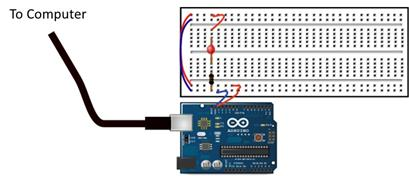
\includegraphics[width=3.4504in,height=1.4955in]{PH4CAU01}
\end{figure}

You are probably familiar with
words like \textquotedblleft voltage\textquotedblright\ and
\textquotedblleft current\textquotedblright\ even though you have not yet
studied these in PH220. You have been plugging in things for many years now.
And so you know that \textquotedblleft voltage\textquotedblright\ has
something to do with electrical energy. That is enough for now. Our voltage
source is just a source of energy to make our circuits work.

A resistor is kind of what it sounds like. It tries to stop or slow down the
electricity in the circuit. The LED is just a circuit element that lights up
when electricity goes through it. You see them on computers and cell phones
as indicators that something has happened.

Let's assemble our system one step at a time.

\subsection{Prototyping boards}

Let's start with your prototyping board.

You might notice that the LED and the resistor in the diagram seems to be
stuck in some strange board full of holes. This is our prototyping board.
You should have one in your Arduino kit. Your instuctor will have several
that you can borrow if you need another one.

We will connect a lot of electrical wires together. We have devices to make
this job easier. Our porototyping board is one of these. They are officially
called prototyping boards, but you might hear them called proto-boards, or
even \textquotedblleft breadboards.\textquotedblright\ They are designed to
allow you to put an electronic element on the board and then connect other
things to that element. The boards look like this. 

\begin{figure}[h!]
	\centering
	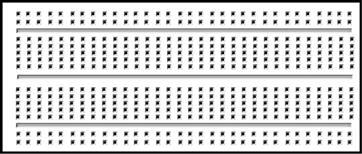
\includegraphics[width=3.0519in,height=1.3102in]{PH4CAU02}
\end{figure}

Notice that in the center of the board there are sets of five holes. Under
the board surface, these holes are connected together as shown by the red
lines in the next figure. 

\begin{figure}[h!]
	\centering
	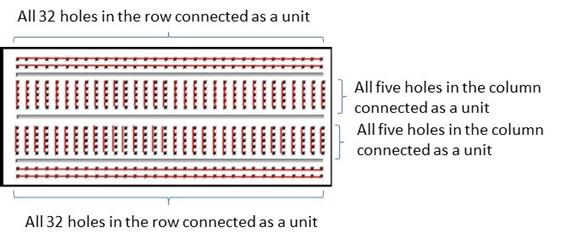
\includegraphics[width=4.8793in,height=2.0384in]{PH4CAU03}
\end{figure} 

Any wire that goes in one of the
connected holes is therefore connected to any other wire that goes in the
set of five connected holes. So you can connect up to four other wires to
the first wire. In the next figure, you can see an example of a resistor
that is placed on the proto-board and is connected to two yellow wires. 

\begin{figure}[h!]
	\centering
	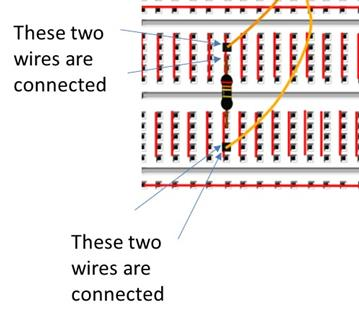
\includegraphics[width=3.0308in,height=2.6947in]{PH4CAU04}
\end{figure}

Notice that each end of the
resistor is connected to a wire by placing the end of the resistor in one of
a set of five connected holes and by placing a wire in another of the set of
five connected holes. This would be a silly circuit to build. There is no
connection to a source of electrical energy. But this gives the idea of how
the prototyping board works.

There are also two long rows of holes on the side of the proto-board. These
are usually all connected along the whole row. 

\begin{figure}[h!]
	\centering
	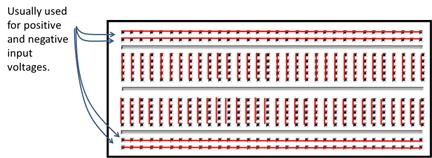
\includegraphics[width=3.6391in,height=1.3439in]{PH4CAU05}
\end{figure}

Not all proto-boards are alike
when it comes to these long rows. But most are connected along the whole
row. These long rows are often used as a convenient way to make input power
available all along the whole board. Of course, once you know how the board
is wired underneath, you can use the connections any way that is consistant
with that design. We could skip using proto-boards and just connect
everything with wires and alligator clips. But proto-boards often make
holding everything in place much easier.

In today's lab experience, let's start by using the long rows as a place for
electrical energy to be used. We have long rows on the top and bottom of the
proto-board. For our first experience, we will use just $0\unit{V}$ and $+5%
\unit{V}.$ Let's make these voltages available on both the top and the
bottom of the board by wiring the two sets of rows together. 

\begin{figure}[h!]
	\centering
	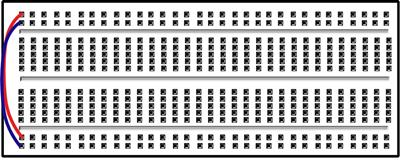
\includegraphics[width=3.3741in,height=1.3615in]{PH4CAU06}
\end{figure}

Looking at our wiring diagram for the inside of the proto-board we can see
that how the top row and the second from the bottom row have been connected
with a wire (it is red if you are reading this in color) and the second from
the top and the bottom row are also wired together (the wire is blue if you
are seeing this in color). And we know that these entire rows are wired
underneath. 
\begin{figure}[h!]
	\centering
	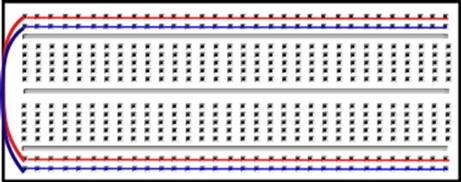
\includegraphics[width=3.4211in,height=1.3615in]{PH4CAU07}
\end{figure}

Some proto-boards even have red
and blue lines to indicate that these rows can be used for electrical power.
Some of ours do.

Next let's add our LED light and our resistor. 

\begin{figure}[h!]
	\centering
	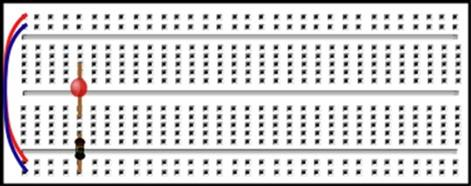
\includegraphics[width=3.9701in,height=1.5806in]{PH4CAU08}
\end{figure}

Notice that the LED\ spans the gap between the top and the bottom of the board.

In the next figure I have included our red connection lines so we can keep
in mind which parts of the proto-board are connected underneath.

\begin{figure}[h!]
		\centering
	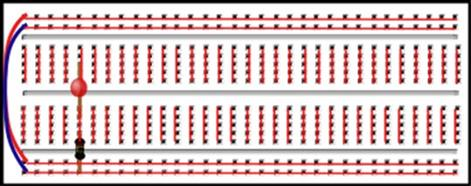
\includegraphics[width=3.9701in,height=1.5806in]{PH4CAU09}
\end{figure}

We placed one LED light wire in one column. On the other side of the board
we place the other wire. The wires that come out of an electronic device are
often called \textquotedblleft leads\textquotedblright\ and I will use this
term. So one LED lead goes in a group of five holes on one side of the board
and the other lead goes into a group of five hole on the other side of the
board. If you look closely, you will see that one side of your LED is flat.
The lead on the flat side should be toward the bottom (toward our $0\unit{V}$
connection that we will make). LED\ lights only work one direction. So when
using LED's, if they don't work, turn them around.

Notice that the way we have done this one LED lead and one resistor lead are
connected in one group of five holes. The resistor is connected to the very
bottom row. The top of the LED is not connected to anything yet. It is in a
set of five holes that are connected together, but we need another wire to
connect the top of the LED to the $+5\unit{V}.$ Let's choose the top of our
power rows to be $+5\unit{V}$ and add the wire to connect the LED. 

\begin{figure}[h!]
	\centering
	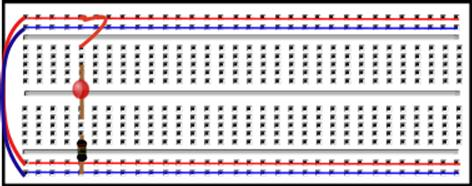
\includegraphics[width=3.979in,height=1.5806in]{PH4CAU0A}
\end{figure}

Now we can wire our light to our Arduino. This will take two wires. One
should be wired to pin13. The pin numbers are given on the side of the
wiring areas. 

\begin{figure}[h!]
	\centering
	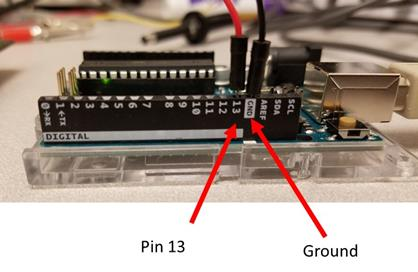
\includegraphics[width=3.5258in,height=2.3017in]{PH4CAU0B}
\end{figure}

This pin 13 is a digital output.
That means it will either have $5\unit{V}$ or it will have $0\unit{V}.$ The $%
5\unit{V}$ will be our \textquotedblleft on\textquotedblright\ value that
could turn on an instrument. In our case it will turn on our LED\ light. The 
$0\unit{V}$ is the \textquotedblleft off\textquotedblright\ value. When pin
13 has a value of $0\unit{V}$ our light will go off. We know that voltage is
related to electrical energy. We will study voltage more next week. But for
now we need to know that voltage is a comparison. So we need to know
\textquotedblleft $5\unit{V}$ compared to what?\textquotedblright\ We
compare to the voltage of the ground. This is literal. Most buildings have a
large copper rod pounded into the ground. All of the plugs in the building
have one of their three wires connected to this rod. Thus they are all
\textquotedblleft grounded.\textquotedblright\ This is our reference. Our
computer is connected to a plug so it is grounded. Our Arduino is connected
to the computer so it is grounded. And one of our pins is a connection to
the ground. It is marked \textquotedblleft GND.\textquotedblright\ This will
be our $0\unit{V}.$ So we need to connect pin 13 and the GND pin to our $+5%
\unit{V}$ and our $0\unit{V}$ rows on our proto-board. The next figure shows
one way to do this.

\begin{figure}[h!]
	\centering
	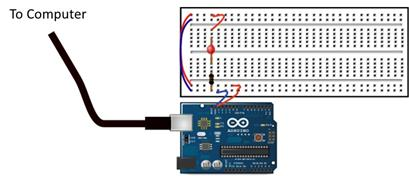
\includegraphics[width=3.4504in,height=1.4955in]{PH4CAU0C}
\end{figure}

We now have hour \textquotedblleft hardware\textquotedblright\ built for
blinking a light. But we need to give instructions to our Arduino that tells
it what to do with pin 13 and pin GND so our light will blink. Our Arduino
has a small computer on board, and we need a computer program to be uploaded
to the Arduino for this small computer to run. We will write and upload that
program next.

\subsection{LED light blink Sketch}

You wrote computer programs in Python in PH150. Our Arduino programs are
similar. They have loops and mathematical statements. There are some
differences as well. Our Arduino programs have special code
\textquotedblleft objects\textquotedblright\ for controlling our Arduino.
Most Arduino programs are very short. We just need instructions to tell the
Arduino what to turn on, turn off, or what data to collect. For today's lab,
we just need to address the digital output pins.

Let me introduce the commands we will use. Each digital output has a number.
The code defines a variable of type integer (int) and sets it equal to the
pin number. That pin can be HIGH or LOW with HIGH $=+5\unit{V}$ and LOW $=0%
\unit{V}$. Each digital pin needs to be set up for output or input. This is
done with a pinMode statement:

\begin{equation*}
	\begin{tabular}{l}
		pinMode(ledPin, OUTPUT)
	\end{tabular}
\end{equation*}
The variable ledPin is the pin number (for us 13). And the key word
\textquotedblleft OUTPUT\textquotedblright\ sets up our pin 13 to turn
things on or off.

To set the pin to HIGH use a digitalWrite command

\begin{equation*}
	\begin{tabular}{l}
		digitalWrite(ledPin,HIGH);
	\end{tabular}
\end{equation*}
and finally, to let the light be on for a while, use a delay command where
the delay time is given in milliseconds (ms)%
\begin{equation*}
	\begin{tabular}{l}
		delay(100);
	\end{tabular}
\end{equation*}

These would not be normal Python commands. They are part of a specific code
library for use in making things with Arduino's.

We have a special development environment for programing our Arduino as
well. It looks like this. 

\begin{figure}[h!]
	\centering
	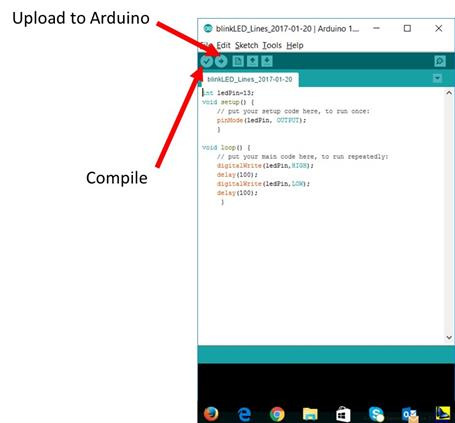
\includegraphics[width=3.8353in,height=3.5674in]{PH4CAU0D}
\end{figure}

We will need to install this
development environment. To do so we go to
https://www.arduino.cc/en/Guide/HomePage and choose to instal the Arduino
IDE for your computer. IDE stands for \textquotedblleft integrated
development environment.\textquotedblright\ This is the environment that you
see in the last figure. It has two unusual buttons on its toolbar. One is
the \textquotedblleft compile\textquotedblright\ button. When you used
Python in PH150, you could run your code by pushing on a green arrow button
in most development environments. If you used Jupyter scripts, they also had
a function to run your code. But our Arduino is not big enough to be able to
run code this way. We need to convert our human-understandable code that
looks mostly like Python into a digital format that the Arduino can
understand. The compile button does this. As the code is converted, the
Arduino software looks for errors in the code. If there are errors, it will
tell you at this point. This is different than Python which only told you
about errors as the code ran. But remember we don't want to run our program
on our computer. We want it to run on our Arduino. So this check is good
before we send the translated code to the Arduino.

We also need a way to send our code to our Arduino and that is what the
upload to Arduino button does. Once the code is compiled without errors,
connect the USB\ cable to the Arduino and push the upload button.

There are also some syntax differences between the Arduino computer language
and Python. If you have taken CS124 or know the \textquotedblleft
C\textquotedblright\ language, you will recognize some of these changes.

\begin{itemize}
	\item Everything in a function needs to be in curly braces \{ \}
	\item Indenting is a good idea, but not required
	\item comments can be started with two slashes //
	\item every line needs a semicolon at the end;
\end{itemize}

\subsection{Arduino LED light blink sketch (program)}

We are ready to write code to blink our LED\ light. Here is an example code.
We write this code right in the Arduino development environment main window. You can download it directly \href{https://dtoliphant.github.io/PH250Manual/Code/IntroBlink.ino}{here}
\lstinputlisting[language=Arduino]{Code/IntroBlink.ino}


%\begin{lstlisting}[language=Arduino]
%/////////////////////////////////////////////////////////
%//Arduino Sketch to blink one LED light
%//   Written by Brother Lines
%//	(place your name here in your code)
%//   Feb 6, 2017
%//
%//   Define our Arduino Variables
%//      We will call pin 13 "ledPin"
%/////////////////////////////////////////////////////////
%int ledPin=13;
% 
%/////////////////////////////////////////////////////////
%// Arduino setup function comes next
%//    Every Arduino sketch needs a setup function
%//    We will set up our ledPin (pin 13) as an output pin
%void setup() {
% // put your setup code here, to run once to set up:
% pinMode(ledPin, OUTPUT);
% }
% 
%/////////////////////////////////////////////////////////
%// Arduino loop function
%//    Every Arduino sketch has a loop function
%//    This is where we put what we want the Arduino to do
%//    The Arduino will do whatever is in the loop function 
%//    until the Arduino is unplugged.
% 
%void loop() {
% // put your main code here, to run repeatedly:
% // turn on the LED
% digitalWrite(ledPin,HIGH);
% 
% // leave in on for 100ms
% delay(100);
% 
% // turn off the LED
% digitalWrite(ledPin,LOW);
% 
% // leave in off for 100ms
% delay(100);
% }
%/////////////////////////////////////////////////////////
%/////////////////////////////////////////////////////////
%\end{lstlisting}

Notice that we used a lot of comments. There are only ten lines that are
actually required to make the sketch run.

\begin{lstlisting}[language=Arduino] 
int ledPin=13;
void setup() {
	 pinMode(ledPin, OUTPUT);
 }
void loop() {
	digitalWrite(ledPin,HIGH);
	delay(100);
	digitalWrite(ledPin,LOW);
	delay(100);
 }
\end{lstlisting}

The comments are not required for the sketch to work, but they help us
remember what we did later. In our class, \textbf{comments are required for
full credit}. So don't leave out the comments. In fact, you can add any
comments that might help you remember why the code works.

Also notice that Arduino programs are called \textquotedblleft
sketches.\textquotedblright\ Most of the commands are special Arduino
commands. And luckily, they make sense when we read them. Try it out. Type
in this sketch including the comments and compile and upload it to your
Arduino. If all goes well, the LED light will begin to blink. If all did go
well, go on to the next section. If it did not, call over an instructor.

Save your sketch and maybe take a photo of your hardware set up. Place both
in your lab notebook along with notes on how you got it to work. We will
build on this sketch, so spend some time documenting what you did in your
lab notebook so you can refer to it later.

\section{Second Computer Control: Two LED blink}

Now let's see if we can apply what we have learned. Let's change our
hardware so that it has two LED lights. Most of the hardware setup will be
the same. But We will wire them to two Arduino pins, say 12 and 13 (along
with GND of course) and have them blink, but blink independently.

We will have to abandon our nice $+5\unit{V}$ top row as our connection to
pin 13 because we need two pins, 12 and 13. The two pins must work
independently. In fact, let's have one LED\ on when the other is off.

This is why we can't wire both LED lights to the top row and wire the top
row to pin 13 as we did last time. That would make both lights blink at
once, but would not let one be off and the other on. Instead, let's wire the
top lead of one LED directly to pin 13 of our Arduino, and let's wire the
top lead of the other LED to pin 12. The two resistors can share a
connection to the GND pin, so let's keep using the $0\unit{V}$ bottom row of
the proto-board. Your hardware should look something like this.

\begin{figure}[h!]
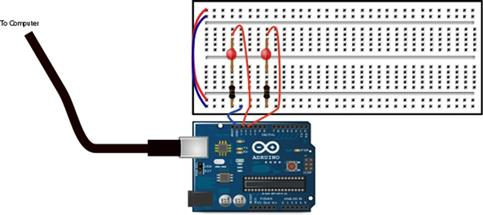
\includegraphics[width=4.0704in,height=1.8228in]{PH4CAU0E}
\end{figure}We will need to modify our sketch
(save the old one first so you have a separate copy for reference). Here is
a suggestion of what the new sketch might look like.

\lstinputlisting[language=Arduino]{Code/IntroBlink2LEDs.ino}


Again save your sketch and maybe take a photo of your hardware set up. Place
both in your lab notebook along with notes on how you got it to work. Make
sure others at your table are able to get their setup to work.

\section{Third Computer Control: Two LED blink using math}

Let's leave our hardware alone in the two LED setup from the last section.
And let's make the LED's blink the same way. But this time, let's calculate
when they should be on or off. Why would we do this? Because sometimes in
computer control of experiments we need to turn something on or off based on
a calculation. You may have your computer watching to make sure the
experiment doesn't get too hot or cold. The Arduino can bring in temperature
information, but you would have to write the code to tell it to turn off the
heater when your experiments gets to hot and to turn it on when it gets too
cold. This could be done with a mathematical comparison. We will use such a
comparison in the next sketch.

Suppose we want to know if a number is even or odd. Even numbers are evenly
divisible by $2.$ We could divide a number by $2$ and see if the remainder
is zero. Our Arduino language has a good set of mathematical functions. The
remainder function is a \textquotedblleft \%\textquotedblright\ sign. For
example 

\begin{eqnarray*}
	3\%2 &=&1 \\
	6\%2 &=&0
\end{eqnarray*}

Let's have one light turn on if a number is even, then switch to the other
light if the number is odd.

In our code we will introduce a variable, $i,$ that we will increment (add
one to) every time the loop runs. So the first time the Arduino loop runs it
will be zero (even) and the next time 1 (odd) and the next time 2 (even) and
the next time 3 (odd) and so on. If you studied Python you would call such a
variable an \textquotedblleft integer\textquotedblright\ and might even know
to call it a \textquotedblleft loop counter.\textquotedblright

In our Arduino sketch we will test to see if $i$ is even in an if-statement.
If-statements go like this
 \begin{lstlisting}[language=Arduino]
 if (test condition ) {
   do something;
 }
 else {
   do something else;
 }
 \end{lstlisting}

Notice that the parts of the if-statement need curly braces. Our condition
to test is
 \begin{lstlisting}[language=Arduino]
i % 2 == 0
 \end{lstlisting}

Note that there are two equals signs. That makes it a test for equality
rather than an assignment. So we will have an if-statement like this
 \begin{lstlisting}[language=Arduino]
if (i % 2 == 0 ) {
 digitalWrite(ledPin1,HIGH);
 digitalWrite(ledPin2,LOW);
 delay(1000);
 }
 else {
 digitalWrite(ledPin1,LOW);
 digitalWrite(ledPin2,HIGH);
 delay(1000);
 }
 
 \end{lstlisting}

One last addition, our Arduino language has a shortcut for the statement
 \begin{lstlisting}[language=Arduino]
i=i+1
 \end{lstlisting}

It is simply
 \begin{lstlisting}[language=Arduino]
i++
 \end{lstlisting}

We will use this to make $i$ increase by one each time the loop runs. The
whole code might look like this.
\lstinputlisting[language=Arduino]{Code/IntroBlink2LEDs_Math.ino}



Again save your sketch. You should probably say in your lab notebook that
you used the previous hardware setup. You might want to describe in your lab
notebook how the mathematical algorithm works.

\section{Fourth Computer Control: Two LED blink in the Fibonacci sequence}

Suppose instead of LED\ lights we had large radio transmitters. And suppose
we were part of the Search for Extra-Terrestrial Intelligence (SETI). We
wish to send a message to any intelligent life that they would understand.
Intelligent life probably would be able to do mathematics and would
understand how mathematics occurs in nature. One sequence of numbers that
occurs over and over again in nature was discovered by Fibonacci. Let's
blink our LED\ lights (representing those powerful radio transmitters) in
the Fibonacci sequence.

We need to know now to calculate the Fibonacci sequence. One method is to
know that the sequence goes like this

\begin{equation*}
	0,1,1,2,3,5,8\ldots
\end{equation*}

and that we can find the next number in the sequence by choosing $f_{1}=0$
first, then $f_{2}=1$ then using the formula 

\begin{equation*}
	f(x-1)\ +\ f(x-2)
\end{equation*}

Let's see that this works. For the first of the sequence, we just write the $
0.$ For the second we just write the $1.$ Then for the third 

\begin{eqnarray*}
	f_{3} &=&f_{2}+f_{1} \\
	&=&1+0 \\
	&=&1
\end{eqnarray*}

So far so good. Let's try the next in the sequence

\begin{eqnarray*}
	f_{4} &=&f_{3}+f_{2} \\
	&=&1+1 \\
	&=&2
\end{eqnarray*}

Again it worked. For the next one

\begin{eqnarray*}
	f_{5} &=&f_{4}+f_{3} \\
	&=&2+1 \\
	&=&3
\end{eqnarray*}

and though we won't prove it, it works for every member of the sequence. See
if you can figure out how to write this code. An example is given below, but
see if you can figure out what the code should be.

This example is a much more complex version of a mathematical based computer
control.
\lstinputlisting[language=Arduino]{Code/IntroFibonacci.ino}
% \begin{lstlisting}[language=Arduino]
%/////////////////////////////////////////////////////////
%// code to blink two LED's using a mathematical expression
%// to determine when they should light. Note that the
%// Arduino code is closer to C++ than python.
%/////////////////////////////////////////////////////////
%int ledPin1=13;
%int ledPin2=12;
%int i=0; //loop counter
% 
%/////////////////////////////////////////////////////////
%int fib_count=0; // number of blinks based on Fibonacci
%int i_max=10; // maximum Fibonacci number before 
% // starting over
% 
%/////////////////////////////////////////////////////////
%void setup() {
% // put your setup code here, to run once:
% pinMode(ledPin1, OUTPUT);
% pinMode(ledPin2, OUTPUT);
% } 
% 
%int fib(int x) {
% // calculates the Fibonacci sequence using recursion
% if (x==0) 
%    return 0;
% if (x==1)
%   return 1;
%   return fib(x-1) + fib(x-2);
% } 
% 
%/////////////////////////////////////////////////////////
%void loop() {
% // put your main code here, to run repeatedly:
% // blink the LED's with the number of blinks being 
% // the Fibonacci sequence.
% fib_count=fib(i);
% if (i % 2 == 0 ) {
%   // turn off one light
%   digitalWrite(ledPin2,LOW);
%   // now blink the second light fib_count times 
%   for (int n=0; n<fib_count; n++) { 
%      digitalWrite(ledPin1,HIGH);
%      delay(100);
%      digitalWrite(ledPin1,LOW);
%      delay(100);
%   }
% }
% else {
%   // turn off the other light
%   digitalWrite(ledPin1,LOW);
%   // now blink the first light fib_count times
%   for (int n=0; n<fib_count ; n++) { 
%      digitalWrite(ledPin2,HIGH);
%      delay(100);
%      digitalWrite(ledPin2,LOW);
%      delay(100);
%   }
% }
% // increment i
% i++;
% // limit our blinks to the first i_max Fibonacci numbers
% if (i>i_max) i=0;
% }
%}
%/////////////////////////////////////////////////////////
%/////////////////////////////////////////////////////////
% \end{lstlisting}

Again save your sketch. You should probably say in your lab notebook that
you used the previous hardware setup. You really should describe in your lab
notebook how the mathematical algorithm works.

For next week, you should read the lab before coming to class. So your
assignment is to read Lab 2.

%TCIMACRO{\TeXButton{\vspace*{\fill}}{\vspace*{\fill}}}%
%BeginExpansion
\vspace*{\fill}%
%EndExpansion
\pagebreak

	
	%\chapter{Introduction to Electrical Measuring Devices (Not Step-by-step)}
		%Intro_El_Measurment
\chapter{Introduction to Electrical Measuring Devices}
\LARGE \textbf{(Not Step-by-step, read before class)}
\normalsize
\vspace{0.25in}

Last week we tackled very simple computer control, but we said we also want
to transfer data from our experiment to our computer. In order to understand
how to do that, we need to know what things we can measure with electronic
devices. We will take on this question today, but we will get practice
making these measurements with special equipment designed just for making
these measurements. These devices won't send the data they measure to our
computers, but they will display it so we can see the data.

Once we know how to make some basic measurements with these stand-alone
instruments, then we can consider how we would make a new instrument to
measure something else. We will build a current measuring device, an \emph{
ammeter} out of electrical components and a \emph{voltmeter}. This will be
something we do over and over again. We will build a new instrument using
instruments we already know, and some electrical equipment.

This lab consists of a large pre-reading section that will give you
background information, and then at the end an assignment where I will ask
you to practice making these measurements with our equipment. Notice this is
different than last week's lab reading. Last week the reading went step by
step through the assignment. This week the assignment is at the end and you
will have to think through how to do the problems as a group.

\section{What we measure: Voltage (and Current)\label{Voltage Measurement
with Meter}}

The two easiest electrical measurements to make are voltage and current
measurements. So physicists try to turn all other types of measurements into
voltage or current measurements. You may want to measure relative humidity.
But to record relative humidity on our computer we need to convert relative
humidity into a voltage or current! We will do experiments that do this type
of conversion, but first, let's learn about voltage and current so we can
see how electronic systems measure them.

Voltage is really ``electrical potential
difference,'' which is the difference between electrical
potential energy per unit charge at two different circuit locations. Last
lab we said voltage was a comparison, and this is the comparison. We compare
the potential energy at two different circuit locations, only we divide the
potential energy by the charge of an electron.

To get a feel for how this works, think of a change in gravitational
potential energy, $\Delta U_{g}$. If we wanted to measure the difference in
potential energy between the top of a hill and the bottom of a hill, we
would need to place some sort of device both at the top and at the bottom of
the hill. 
\begin{figure}[h!]
	\centering
	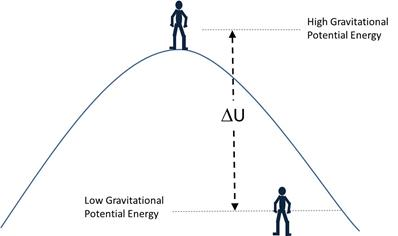
\includegraphics[width=3.3537in,height=1.9977in]{PH4CAU0F}
\end{figure}

We have to do the same thing in
our electrical case. We need two ``probes,'' one placed at the high potential and one placed
at the low potential. For example, we could have the circuit that you see in the next figure.

\begin{figure}[h!]
	\centering
	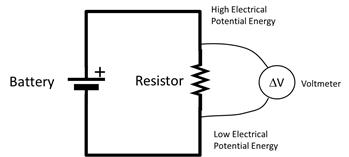
\includegraphics[width=2.9438in,height=1.3353in]{PH4CAU0G}
\end{figure}

The positive end of the battery is like the top of the hill. It provides a high electrical potential energy. So we put one probe at the top of the ``hill'' or the plus side of the battery, and the other on the bottom of the ``hill'' or minus side of the battery. The negative side of the battery provides a low electrical potential energy. With this we measure how high our potential
``hill'' is. The difference between these two measurements is called \emph{voltage.} You should ask yourself
``what would happen if you got the probes
backward?''

In the next figure you can see how to actually perform this voltage measurement with one of our meters.

\begin{figure}[h!]
	\centering
    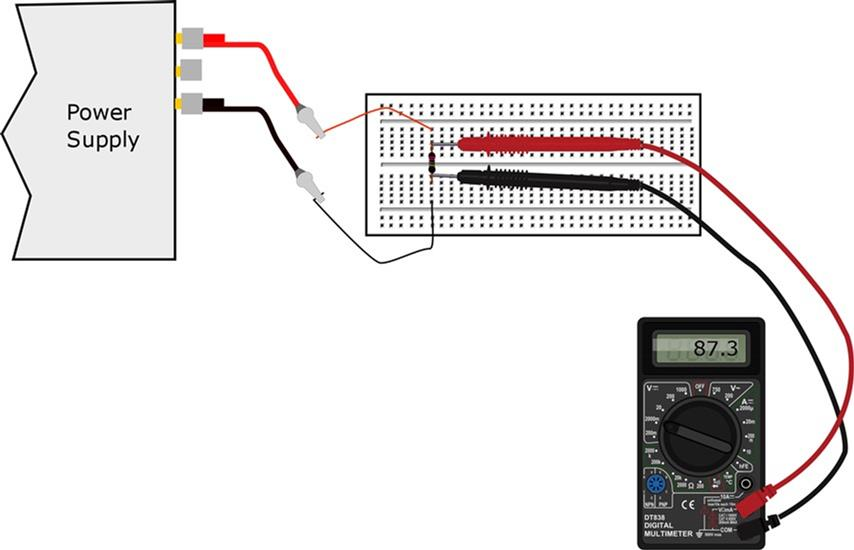
\includegraphics[width=5.5997in,height=3.614in]{PH4CAU0H}
\end{figure}

We say we measure voltage ``across'' a circuit element. This makes some sense if you consider that we very seldom stand batteries up so their electric potential is greater in the same direction as their gravitational potential. Batteries, resisters, capacitors, etc, often lie down, and we measure ``across'' them by putting the positive probe on the high potential side and the negative probe on the low potential side. Even though the battery is lying down, we are still measuring a higher and lower potential energy difference. Knowing a little about voltage, let's look at our devices that produce voltages and then the devices that measure voltages.

\section{Stand-Alone Experimental Hardware}

In today's lab we will study four hardware devices. It might be better to skim this part before lab, then read it in detail with your lab group in class when you have the equipment in front of you. \textbf{But do read these sections!} You can damage your equipment if you don't know how the equipment works. So read these sections as you work! And you need to read the sections about  designing new measuring devices below (starting in section \ref*{New_Instrument_Section}), so skim the equipment sections, but not the rest!

Here is a list of the devices we will study in this time's lab:
\begin{enumerate} 
	\item a power supply
	\item a signal generator
	\item a multimeter
	\item an oscilloscope.
\end{enumerate}

We will call these ``stand alone'' instruments because they are independent boxes that do their job of measuring or generating signals without a computer connected to them. The power supply and the signal generator make voltage signals. The other two devices measure them. Let's look at the power supply and signal generator first, then take on the measuring devices.

\subsection{Power Supply}

A power supply is like an adjustable battery. Batteries have fixed voltages. But a power supply may have an adjustable voltage. 

\begin{figure}[h!]
	\centering
	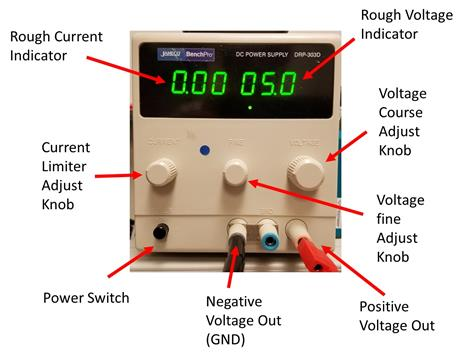
\includegraphics[width=3.9237in,height=%
3.0191in]{PH4CAU0I}
\end{figure}

Usually a power supply takes electrical energy from the wall outlets and converts that energy into the specific voltage that we want for our experiment. So it is like a battery, but must be plugged into the wall. Our power supplies are designed to keep us safe. They are current limited, meaning that they try not to give too much charge flowing through our wires. Sometimes this is a problem
because they are too limited. There is a current limiting knob that you can turn to allow a little more current. Be careful when you use this. The voltage may jump wildly when you turn the current knob! It is best to turn all the knobs down as low as they will go before you turn on the power
supply. Then, after turning on the power supply, increase the current knob about half a turn and then slowly turn the voltage knob up to your desired voltage. If the voltage stops increasing, turn the voltage knob back down a bit, and turn up your current limiter knob some more. Then try your voltage knob again.

Some of our electrical devices are quite delicate, and will literally burn up if you apply too much current or voltage. In today's lab, we will practice using our power supply so we are prepared when the delicate components come out later.

\subsection{Signal Generator}

\begin{figure}[h!]
	\centering
	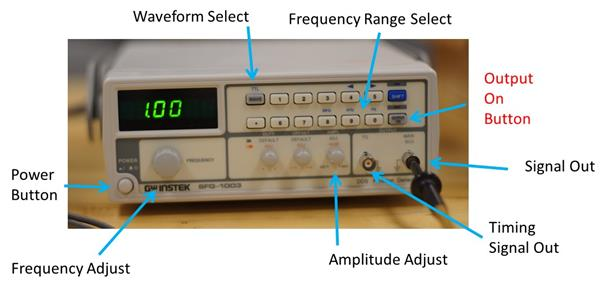
\includegraphics[width=5.093in,height=3.0in]{PH4CAU0J}
\end{figure}

The signal generator is a fancy power supply. It makes changing voltages. It can make voltages in sine, square, and triangle patterns. These time-varying signals have a maximum voltage (called the amplitude) . We will use both the wave output and a timing signal that the wave generator creates. Each has their own Bayonet Neill--Concelman connector (usually just called a BNC connector) on the
front of the signal generator. You will need a cable with BNC connectors on one end (and maybe alligator clips on the other end) to use this device. There is an amplitude knob on the front of the signal generator. Because the signal generator makes a voltage that changes in time, the amplitude of the signal must be in voltage units. We should be careful not to set the signal amplitude (voltage) too high or we run the risk of destroying our measuring devices. Again turn the amplitude (voltage) down before you connect the box to our electrical components. Then turn up the voltage to what you want in a safe way.

There are frequency range buttons (using the shift button) near the middle of the device panel. To change the frequency, you use the shift and range buttons to set which digit you are adjusting, then turn the frequency knob to make the change. An annoying feature of our frequency generators is that you must push the ``output on'' button or they don't output a signal. When everything is set up right, we get a sine wave (or square wave, or triangle wave) out. Here is a signal from the signal generator displayed on one of our measuring devices, the
oscilloscope. 

\begin{figure}[h!]
    \centering
    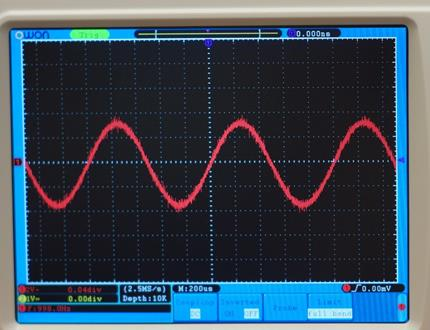
\includegraphics[width=3.0in,height=2.0in]{PH4CAU0K}
\end{figure}

Of course, simple batteries are sources of voltage, and so are many other things.

\subsection{Voltmeter}

Our first measurement device is voltmeter. It measures the electric potential (voltage) between its two leads (sometimes called ``probes'' ). Here is a picture of one of our multi-meters set to measure voltage.

\begin{figure}[h!]
	\centering
	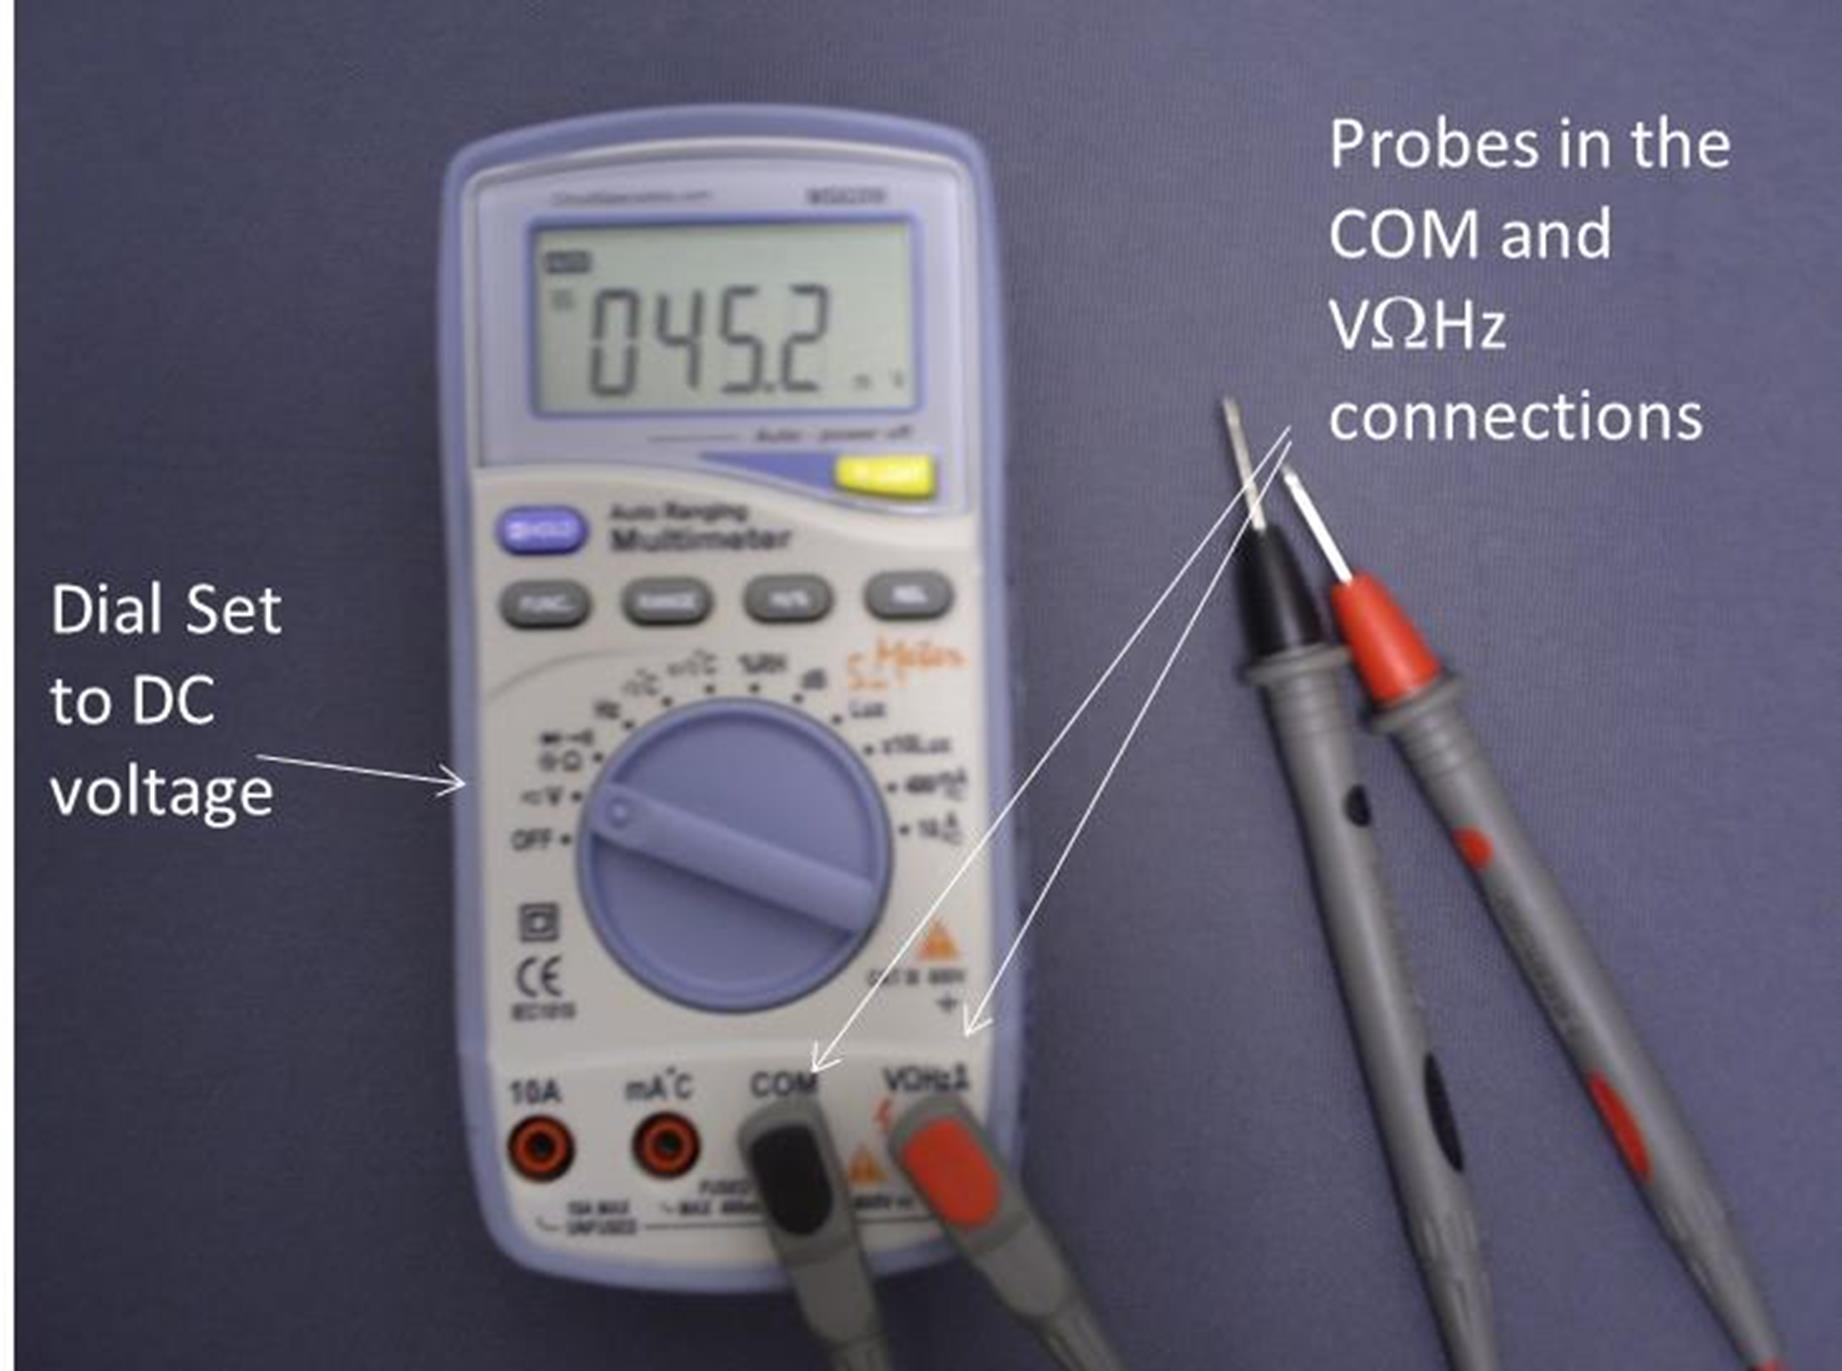
\includegraphics[width=3.116in,height=2.3266in]{PH4CAU0L}
\end{figure}

The display is set to read voltage by turning the dial to the $\unit{V}$ position. There are often two voltage settings. The one that has a wavy line next to it is alternating voltage. The one that has a straight line with three dots under it is the direct current (DC) voltage. These words might not mean much to you yet if you are just starting PH220. So for now, we will just use the DC voltage setting. As you learn more, we may use the alternating voltage setting. The leads (probes) should be connected to the COM (common) and $\unit{V}\unit{\Omega}\unit{Hz}$ connectors. Note that connecting your probe leads to the wrong position can blow the fuse (or worse) in your meter and make subsequent readings very wrong. You should make sure you don't do this, and watch to make sure someone else has not done this before you. If the meter seems crazy, it just may be. We have several different voltmeter models. Here is a picture of a different model.

\begin{figure}[h!]
   \centering
   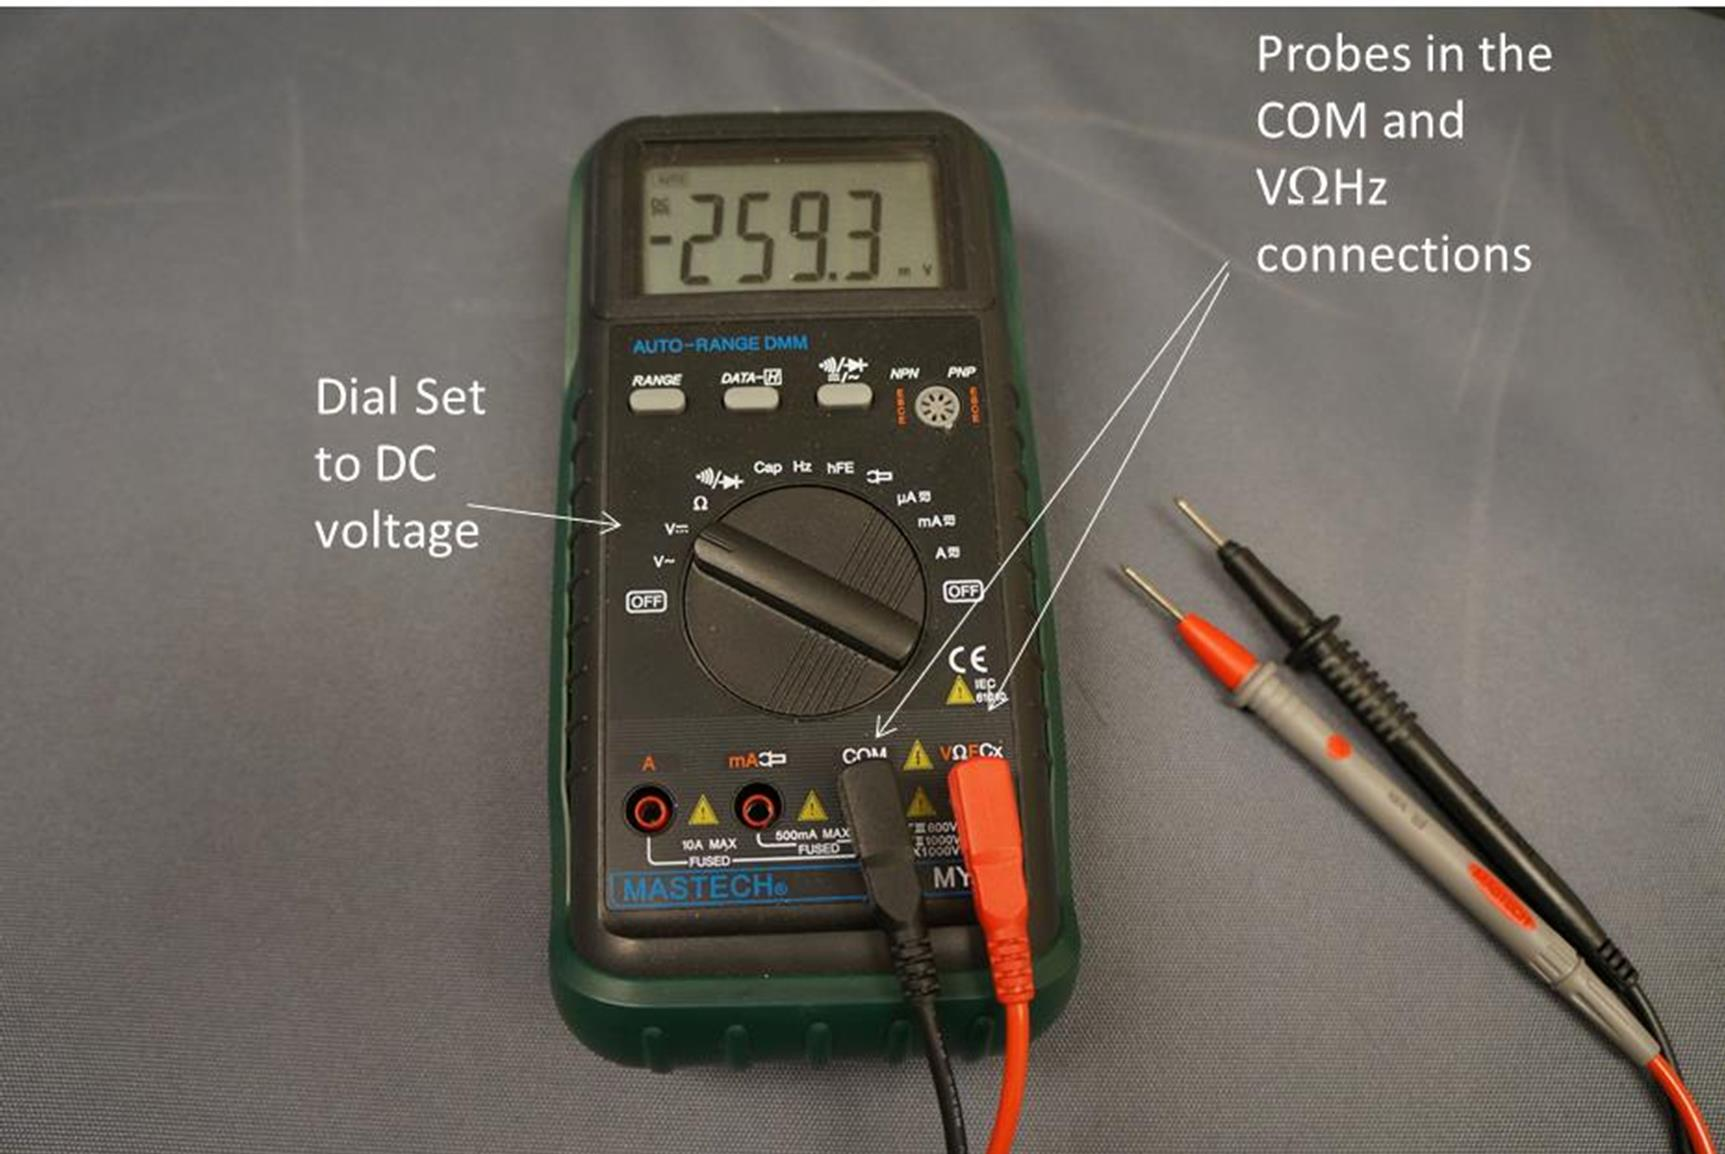
\includegraphics[width=2.9199in,height=1.962in]{PH4CAU0M}
\end{figure}

You will notice that there are other settings besides volts. Our meters are all multi-meters. That means that they can measure more than one thing. We will use several of the settings throughout the semester.

\subsection{Oscilloscope}

Our next device, the oscilloscope, is just a fancy voltmeter. Unlike the multimeter, it usually just measures voltage. But it does it with flare!

The oscilloscope can measure changing voltages very accurately and usually has a way to graph the changing voltage. The standard is a voltage vs. time graph. A sinusoidally varying voltage should look something like this when plotted. 

\begin{figure}[h!]
	\centering
    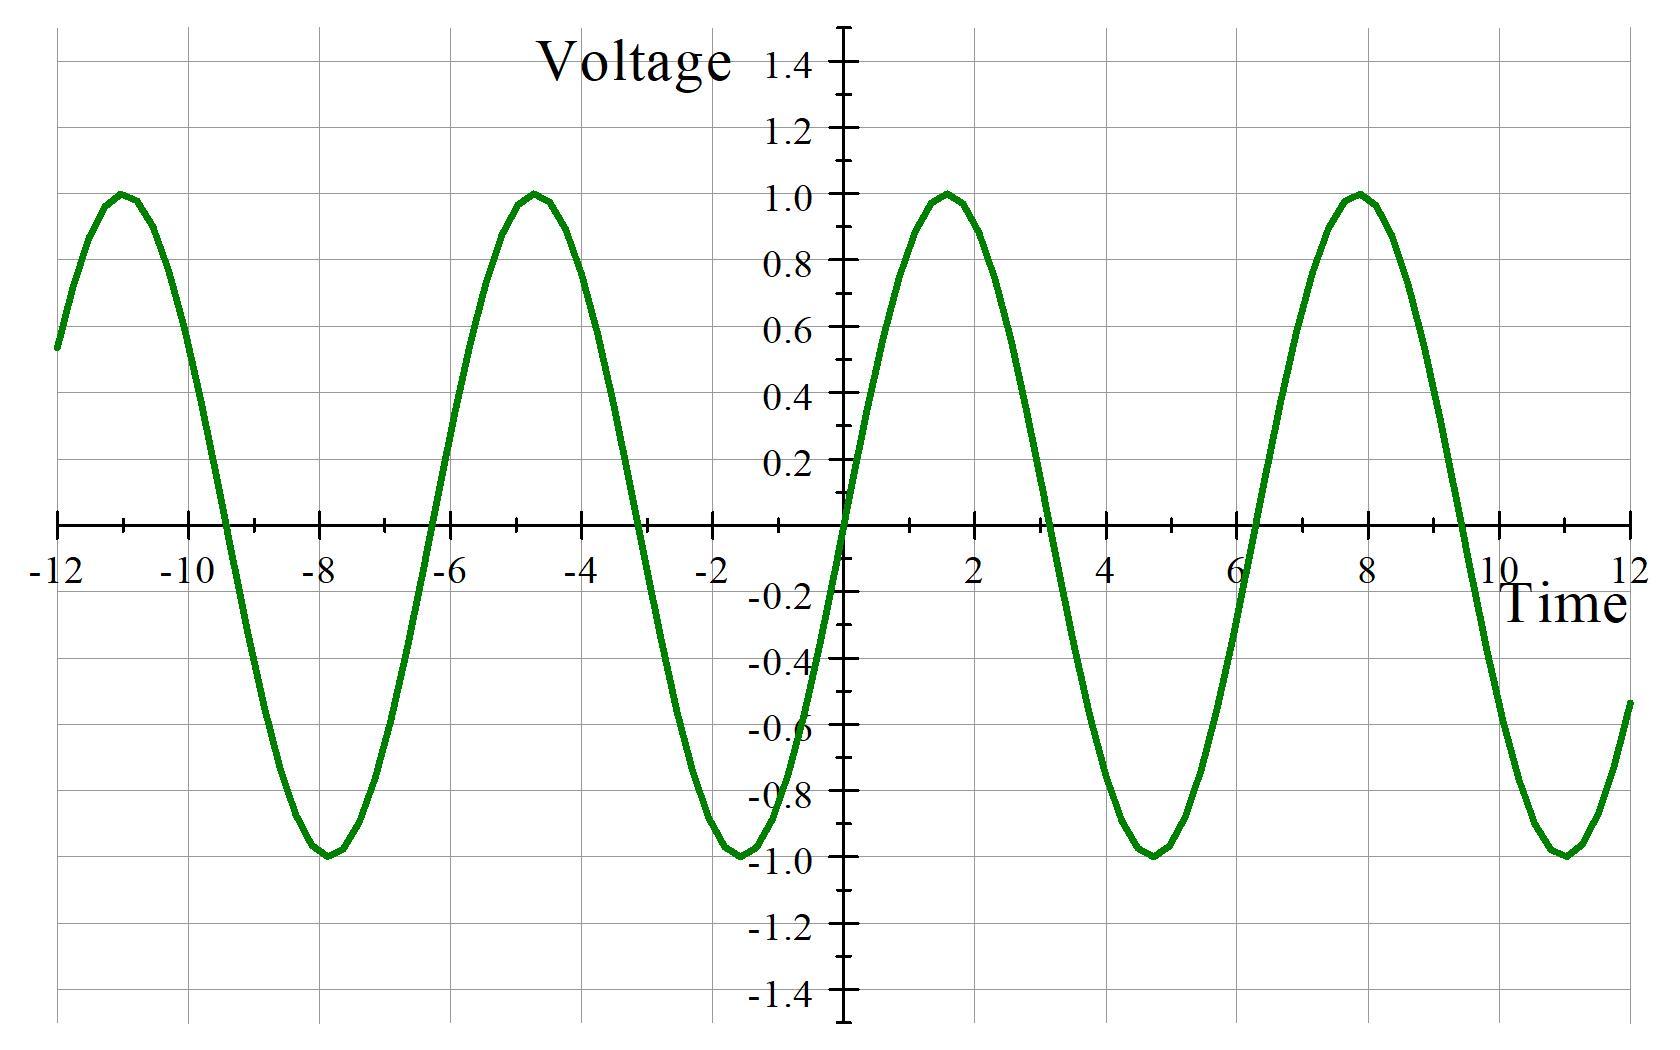
\includegraphics[width=3.00in,height=2in]{PH4CAU0N}
\end{figure}

And that is what our oscilloscope does. We should see something like this on the oscilloscope screen. From our discussion of the signal generator, you know that this is just what we see.

\begin{figure}[h!]
	\centering
    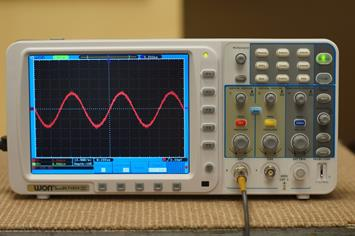
\includegraphics[width=3.00in,height=2.00in]{PH4CAU0O}
\end{figure}

If the changing voltage is periodic, the oscilloscope has a way to use this fact to stabilize the graph so you can see the details more clearly. This stabilization is called ``triggering'' and
on our oscilloscopes there are buttons and knobs on the right hand side of the oscilloscope that adjust the triggering to make the graph more stable (or less stable). The photograph of the sine wave above was taken by stabilizing a sine wave from our signal generator. The oscilloscope starts
plotting at the same part of the wave each time, so the periodic signal seems to stand still. To do this we must ``trigger'' the graph at some good starting point. Our oscilloscopes have a build-in circuit that can watch for the same part of a signal and start the graph in the same place each time. One of the knobs adjusts the trigger point. 

\begin{figure}[h!]
	\centering
    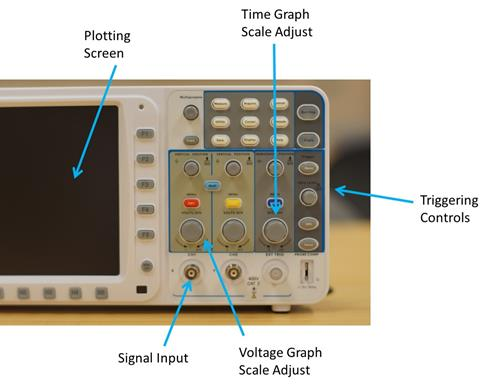
\includegraphics[width=4.00in,height=3.00in]{PH4CAU0P}
\end{figure}

The other controls adjust the horizontal and vertical axes. The vertical axis is voltage, and the voltage axis control is next to the signal input toward the bottom middle of the front panel. To the right of this is the horizontal axis control, which is time. You can choose how many volts per division with one knob and how many seconds (or fractions of seconds) per division you have on your graph with another knob. In the next figure you can see a signal on the oscilloscope screen. 

\begin{figure}[h!]
	\centering
	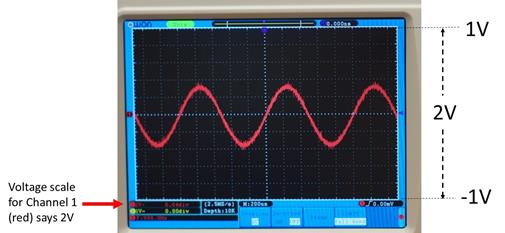
\includegraphics[width=4.2505in,height=1.9718in]{PH4CAU0Q}
\end{figure}

In the bottom left-hand corner there is a red dot and a voltage given. This is the voltage displayed across the whole screen. Since when this photo was take the voltage knob was set to 
$2\unit{V}$, this means that the bottom of the screen represents $-1\unit{V}$ and the top of the screen represents $+1\unit{V}.$ 

\begin{figure}[h!]
	\centering
	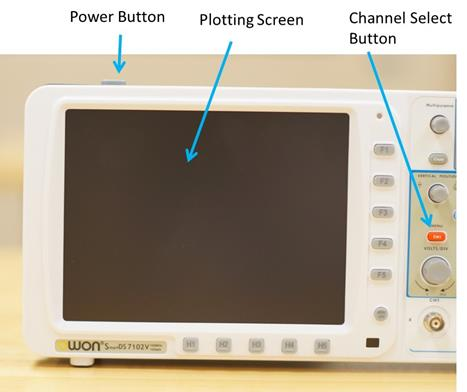
\includegraphics[width=3.9364in,height=3.3076in]{PH4CAU0R}
\end{figure}

There are two signal inputs because our oscilloscopes can look at two different voltage signals at the same time. Each signal input is called a ``channel.'' Each channel has it's own voltage scale knob and voltage scale indicator in the bottom left-hand corner. They share the same time scale.

The channel inputs each have a BNC connector. We use oscilloscope probes connected to these connectors. Notice that since there are two channels, an oscilloscope can measure two voltages at once. But that means we may need two probes!

To check that our oscilloscope is working correctly we can measure a known voltage, say, the voltage of a regular battery.

\begin{figure}[h!]
	\centering
	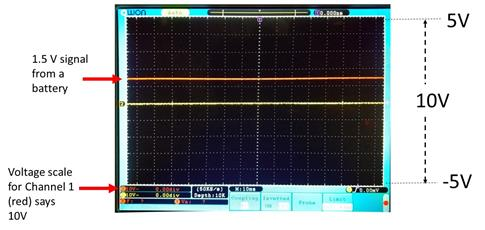
\includegraphics[width=4.0836in,height=1.9458in]{PH4CAU0S}
\end{figure}

Notice that I changed the voltage scale knob position so that now the oscilloscope screen has a $10\unit{V}$ total potential change. That means that we have $5\unit{V}$ at the top of the screen and $-5\unit{V}$ at the bottom of the screen. The screen is divided into little boxes. There are five rows of boxes from the bottom to the top of the screen. Each box represents $1/10$ of the total voltage. Since we have $\Delta V=10\unit{V},$ each box represents $\Delta V=1\unit{V}. $ So our battery voltage should give us one and a half boxes. And that is just what we got.

But sometimes the oscilloscope does not get the right voltage. If this happens we need to calibrate the oscilloscope. Every time we use an Oscilloscope it is a good idea to check it to make sure it working well. Our oscilloscopes have a test voltage to use just for this purpose.

\begin{figure}[h!]
    \centering
    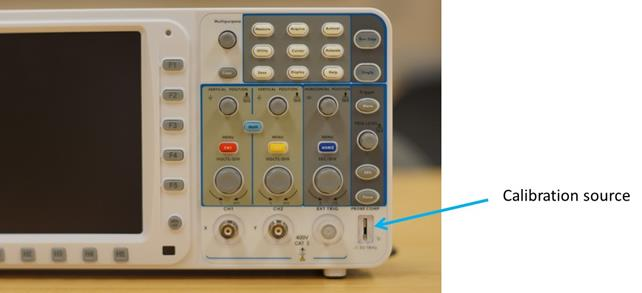
\includegraphics[width=3.70in,height=1.50in]{PH4CAU0T}
\end{figure}

The calibration source makes a $5\unit{V}$ square wave (try it to see what that looks like!). If we use this calibration source we should get something like what you see in the next figure. 

\begin{figure}[h!]
	\centering
    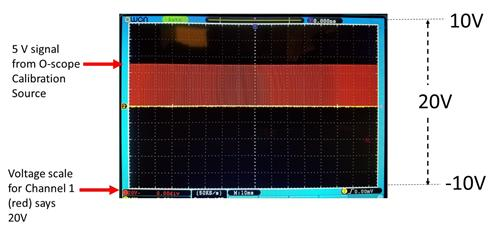
\includegraphics[width=4.00in,height=2.00in]{PH4CAU0U}
\end{figure}

If you don't get $5\unit{V},$ then some thing is wrong and you will need to go through the oscilloscope's calibration procedure. That is in the oscilloscope manual and you can find
the manual on-line.

\section{Current}

Our multimeters have a current setting as well as a voltage setting. Current is a flow of charge. This is like a water current, which is a flow of water. Only we have a different thing flowing. We have a flow of charge. In the wires in our Arduino, the moving charged things are (mostly) electrons. We can write the flow of something as 

\begin{equation*}
	I=\frac{\Delta Q}{\Delta t}
\end{equation*}

where for us $\Delta Q$ is the amount of charge that has gone by in the time 
$\Delta t.$ Physicists use the letter $I$ for electrical current.

We should take a minute to think about what to expect when we allow charge to flow. Think of a garden hose. If the hose is full of water, then when we open the faucet, water immediately comes out. The water that leaves the faucet is far from the open end of the hose, though. We have to wait for it to travel the entire length of the hose. But we get water out of the hose immediately! Why? 

\begin{figure}[h!]
	\centering
    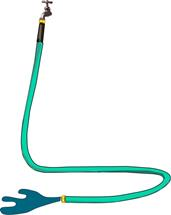
\includegraphics[width=1.4547in,height=1.8228in]{PH4CAU0V}
\end{figure}

The new water coming in causes a pressure change that is transmitted through the hose. The water at the open end is pushed out. You can tell this is the case because the water immediately leaving the hose is warm and tastes like plastic hose. After a while, the water is colder and cleaner.

Current is a little bit like this. When we flip a light switch, the electrons near the switch start to flow. But there are already free electrons in the wire. These experience a push that makes the light turn on almost instantly. But the electrons that turn on the light are not the ones
that just went through the switch. 

\subsection{Measuring Current}

Because current is a flow, to measure current we must put a meter into that flow. In a house, if you want to measure how much water is used, you connect the pipe from the city water system to a meter and then connect the meter to your house. The water flows through the meter and then goes into the pipe that brings water to the house. That way, the meter can't miss any of the water (and the city can't miss any of your payment!). The same is true for electrical current. To measure electrical current, we need to remove part of our circuit, and replace it with the meter to force the flow of electrical current to go through the meter. A schematic diagram of this might look like this: 

\begin{figure}[h!]
	\centering
    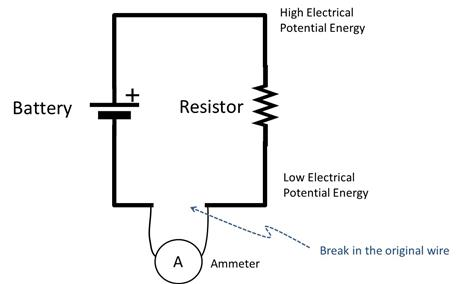
\includegraphics[width=3.8484in,height=2.3981in]{PH4CAU0W}
\end{figure}

In this diagram, you can see that the electric current must go through the current meter. In fact, it couldn't go anywhere else because part of the original circuit wire is missing. This is just what we want. To actually perform this measurement with one of our multimeters you could set up a circuit like the one in the following figure. 

\begin{figure}[h!]
	\centering
    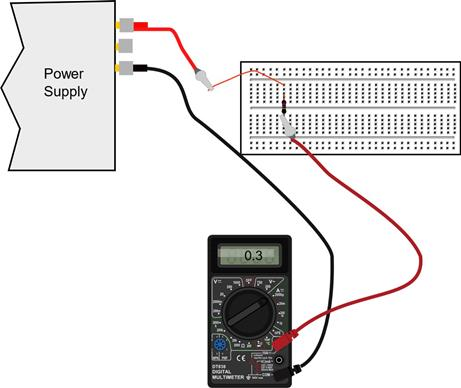
\includegraphics[width=3.8821in,height=3.2707in]{PH4CAU0X}
\end{figure}

There is one more important thing to do to make this work. We need to change the meter settings. And there are two separate changes. The first is to switch the probe connections. One probe stays in the COM or common connector, but the other needs to move to the connector marked with an ``A.'' Here is an example showing the changes with two kinds of multimeters. 

\begin{figure}[h!]
    \centering
    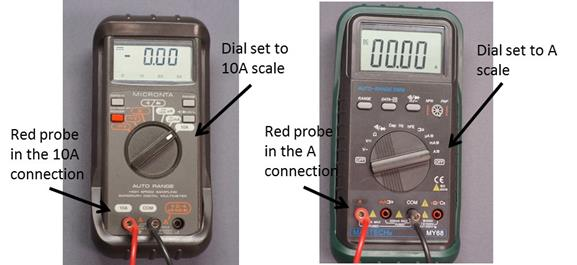
\includegraphics[width=4.858in,height=2.2423in]{PH4CAU0Y}
\end{figure}

The ``A'' stands for the standard unit of electrical current, the Ampere or Amp. With the multimeter set up like this we would call it an \emph{ammeter}. Ammeters measure electrical current.

\section{Building a New Instrument} \label{New_Instrument_Section}

We said before that physicists like to change any measurement they can into a voltage measurement. That is because we have devices like our Arduino boards that measure voltage. We build new instruments by finding ways to turn the measurement that we want to make into a voltage.

In order to build a new instrument, we need to understand the quantity that we really want to measure. We will need to understand the physics of the quantity to make a good new instrument design. Let's take an example. Suppose we wish to measure current, but suppose we don't have a current setting on our Arduino (because we don't). Could we still make a current measurement?

The secret of instrument design is to understand the physics of the measurement we want to make (current) and then see if we can turn that measurement into a voltage.

\subsection{Start with the Physics:}

Let's keep thinking of current like water in a hose. Will there be any friction associated with the water traveling through the hose? Of course there will! We usually call friction in fluids \emph{viscosity}. But it is a form of friction, and we can use our PH121 intuition about friction to see how it would work. Think of having two hoses, one twice as long as the other. Which would you expect to have more friction? 

\begin{figure}[h!]
	\centering
    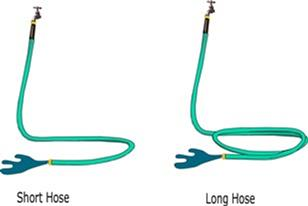
\includegraphics[width=2.6033in,height=1.7474in]{PH4CAU0Z}
\end{figure}

Our friction experience says that the longer the path, the more the friction. The current has longer to interact with the hose, so it experiences more friction. Electrical currents are like this. Longer wires give more friction.

George Simon Ohm noticed that with long metal wires, there seemed to be a linear relationship between the potential difference (voltage), the current, and the length of the wire. The longer the wire, the less the current. His work was confirmed and expanded on by others, who found that not only length mattered, but also the diameter of the wire mattered. The relationship is now expressed as

\begin{equation*}
	\Delta V=IR
\end{equation*}

$\Delta V$ is our old friend, voltage, and we know $I$ is the symbol for current, and $R$ is the slope of the $\Delta V$ vs. $I$ curve. The experiments showed this constant $R$ depended on the material. It is like our viscosity in hoses. It is the friction. The more the friction, the harder it is to get the current through the wire. But like we don't call viscosity ``friction,'' we also don't use the word ``friction'' for this friction-like term. We call it \emph{resistance.} We could solve for this resistance 

\begin{equation*}
	R=\frac{\Delta V}{I}
\end{equation*}

or we could plot $\Delta V$ vs. $I$ and the slope of this line would be the resistance.

\begin{figure}[h!]
	\centering
	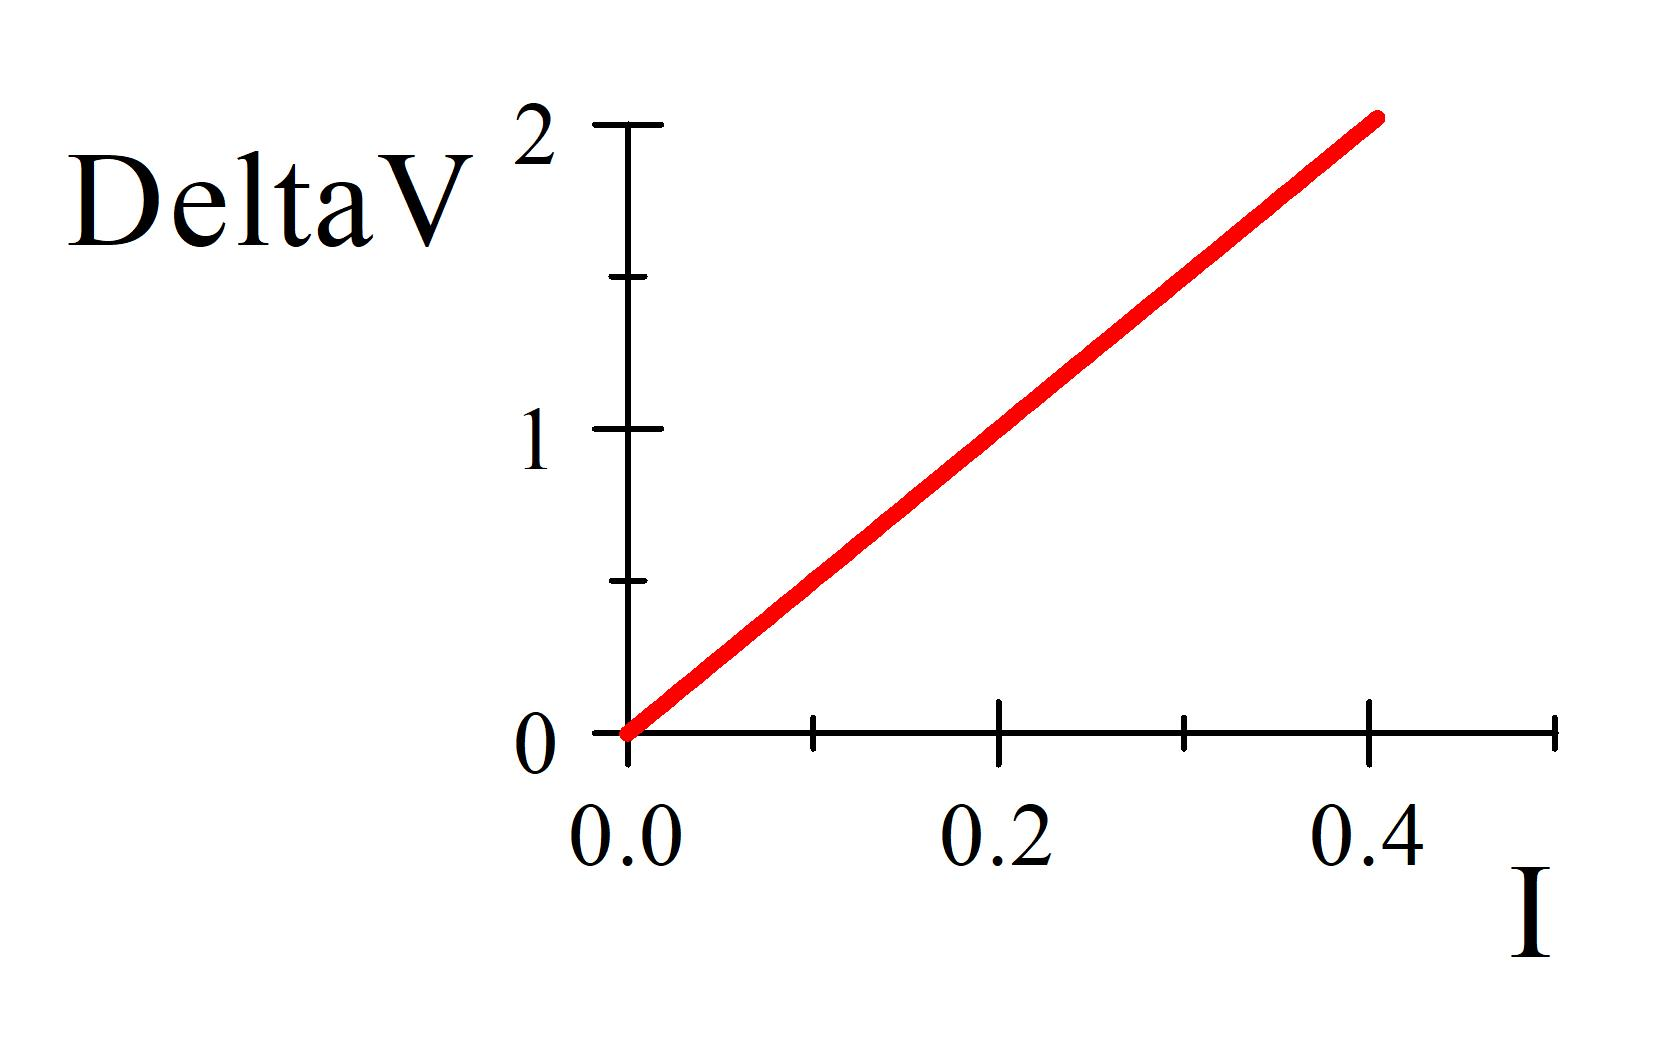
\includegraphics[width=1.9899in,height=1.3214in]{PH4CAU10}
\end{figure}

Either way, this relationship tells us that it takes more potential energy to get the same current if there is more resistance.

This is called \emph{Ohm's law.} The relationship holds well for metals and many materials, but, like Hook's law, this ``law'' does not always hold. Devices that do provide a constant resistance coefficient, $R,$ are called \emph{resisters.} We will use this symbol

\begin{figure}[h!]
	\centering
    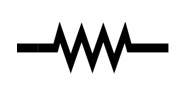
\includegraphics[width=1.742in,height=0.2794in]{Resister_symbol0}
\end{figure}

for resistors, but they often look more like this

\begin{figure}[h!]
	\centering
    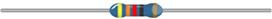
\includegraphics[width=2.2987in,height=0.179in]{PH4CAU11}
\end{figure}

Notice that this is important! We have found a way to relate our new quantity that we want to measure, current, to a voltage. We know how to measure a voltage! Our Ohm's law equation even tells us what extra part we need to convert our voltmeter into a current measuring instrument. We will need a resistor.

\subsubsection{Resistor Code}

Let's pause in our new instrument design for a moment and ask, ``how would you know the resistance of a resistor?'' Our multimeters have a resistance measuring setting, so you could measure the resistance directly using the meter. But many commercially produced resistors come conveniently marked with a color code that helps you identify their resistance. The basics of the color code are given in the following figure\bigskip 

\begin{figure}[h!]
	\centering
    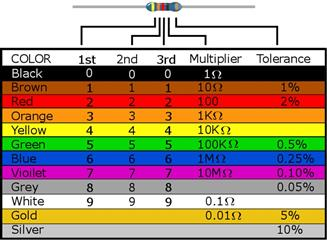
\includegraphics[width=3.2958in,height=2.4249in]{PH4CAU12}
\end{figure}

To use the code:

\begin{enumerate}
    \item Find the tolerance code band. This band is usually brown in our kit resistors and often is set off from the others a little more.

    \item Read the first color band from the side opposite the tolerance band. This will be the first digit of your resistance. I\ think the example resister on the chart has a yellow first color band, so the first digit of our resistance is $4.$

    \item Read the second color band. This will be the second digit of your resistance. I\ think the second band of our example resistor is orange, so the second digit would be a $3,$ making our resistance so far $43$

    \item Read the third color band. This will be the third digit of your resistance. I\ think the second band of our example resistor is red, so the second digit would be a $2,$ making our resistance so far $432$

    \item Read the forth color band. This is a multiplier. You multiply the first three digits by this amount. For our example resistance, I think the third band is black. Then we multiply $432$ by $1\unit{\Omega}$ to get $432\unit{\Omega}.$ This is our resistance.

    \item The tolerance band gives the uncertainty in this value. Our example resistor seems to have a brown tolerance band, which tells us our value is good to $\pm 1\%.$ For our example resistance, $1\%$ would be $0.01\times 432\unit{\Omega}=\allowbreak 4.\,\allowbreak 32\unit{\Omega},$ so our resistance is $\left( 432\pm 4\unit{\Omega}\right) .$
\end{enumerate}

We won't memorize the resistor code, but you should be able to find a resistance using the code.

If you are in doubt about what color you see on a resistor, our multimeters can measure resistance directly. 

\begin{figure}[h!]
	\centering
    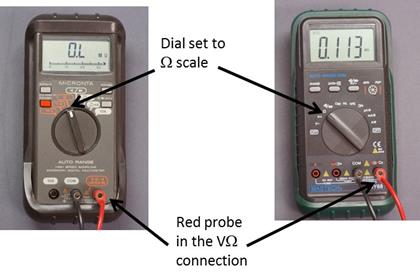
\includegraphics[width=3.5426in,height=2.3594in]{PH4CAU13}
\end{figure}

Place the red probe in the connector with a $\Omega $ marked on it and turn the dial to the $\Omega$ setting. Place the probes on either side of the resistance to be measured. Be careful/ You are a resistor too. If you touch your hands to the probes (common mistake while you try to hold the resistor on the probe ends) you may measure your resistance instead of the resistor's! You have a resistance of around half a megaohm. This is a general concern, every time you measure resistance with a meter you need to take the circuit element (resistor, light bulb, whatever) out of the circuit and measure it on it's own. Otherwise, you might be measuring the resistance of the rest of the circuit. Alligator clips are useful for this.

\subsubsection{Direction of current flow}

If you are half way through PH220 when you take this lab you will already know about current direction and can skip this section. \textbf{But if you are at the beginning of PH220, read on!} There is a historical oddity with current flow. That is that the current direction is the direction positive charges would flow. This may seem strange, since in good conductors electrons are doing the flowing and they are negative! The electrons go the opposite way the current goes. 

\begin{figure}[h!]
	\centering
     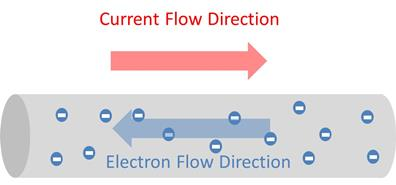
\includegraphics[width=3.3373in,height=1.5696in]{PH4CAU14}
\end{figure}

The truth is that it is very hard to tell the difference between positive charge flow and negative charge flow the other direction. In fact, only one experiment that I know of shows that the charge carriers in metals are electrons. And mathematically, the flow of electrons one direction is equivalent to the flow of positive charges the other direction.

\begin{figure}[h!]
     \centering
     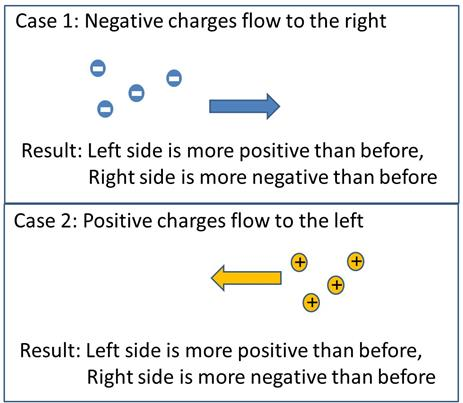
\includegraphics[width=3.8994in,height=3.3961in]{PH4CAU15}
\end{figure}

Worse yet, in biological things it \emph{is} positive ions that flow. So for biology a positive charge carrier is just fine.

Ben Franklin chose the direction we now use. He had a 50\% chance of making it easy for our electronics lab. But he got it backwards for us (but right for biology--and how many electronic things did Ben Franklin have anyway?). All this shows just how hard it is to deal with all these things we can't see or touch that we study in PH 220.

And even more importantly, in semiconductors--special electronic devices in all computers and in our Arduinos--it \emph{is} positive charge that flows. In many electrochemical reactions \emph{both} positive and negative charges flow. So Mr. Franklin was not really so very wrong. We will stick with the convention that \textbf{the current direction is the direction that positive charges would flow regardless of the actual charge carrier motion.} If you are like me, this will seem a little backwards, but we all get used to it.

But what makes the electrons or positive charges want to flow in the first place? We know the answer to this from earlier in this lab reading. It is potential energy. When we connect a metal wire to the terminals of a battery we know that the charges in the metal wire ends will experience a difference in potential energy. The potential energy difference will set up an electric field inside the conductor. 

\begin{figure}[h!]
	\centering
    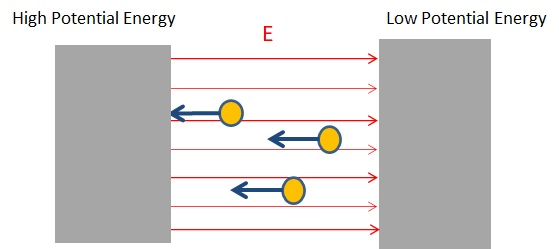
\includegraphics[width=4.2832in,height=1.53in]{PH4CAU16}
\end{figure}

This field makes the free charges move! It causes a force on the little electrons. We won't have to measure any fields in our lab today, but you should know they are there. The important thing is to realize that voltages produce currents. And the amount of current is proportional to the amount of
voltage. This is just Ohm's law! 

\begin{equation*}
	\Delta V=IR
\end{equation*}

The constant of proportionality is related to how much friction there is for the charges in the wire.

\begin{equation*}
	I=\frac{1}{R}\Delta V
\end{equation*}

It is just the resistance, $R$.\ 

\subsection{Knowing the Physics, Design the new instrument}

Now that we understand electrical current, we have some hope of figuring out how to build an instrument to measure that electrical current. From what we learned, consider adding in an additional small resistor in our circuit. If we take a small resistance, one that is small compared to all the other resistances in the circuit, and we put it in the circuit it will slow down the current, but not by very much. If the resistance is small enough, we won't even notice the change. Then if we measure the voltage across that small resistor with a voltmeter, we could mathematically calculate how much current we have. Notice that this instrument design has two parts. The first is adding some new hardware to our voltmeter (a resistor) and the second is adding in some calculation to get our voltmeter reading converted into current. Here is our equation for the calculation

\begin{equation*}
I=\frac{1}{R}\Delta V
\end{equation*}

And let's give this new additional small resistor a name. Let's call it the ``shunt resistor.''

\begin{equation*}
	I=\frac{\Delta V_{meter}}{R_{shunt}}
\end{equation*}

Today we will have to do the calculation part by hand. In future labs, we would carefully plan for this calculation in our Arduino sketch code.

\begin{figure}[h!]
	\centering
    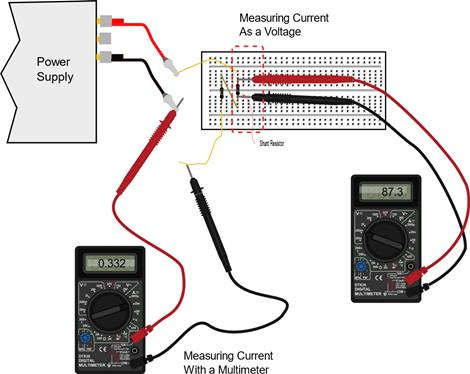
\includegraphics[width=4.9156in,height=3.9176in]{PH4CAU17}
\end{figure}

When we are done wiring our new instrument, we will have done something really cool. We have turned our current measurement into a voltage measurement plus a calculation. We measured something new in terms of a measurement we already knew how to make. We will generally try to do this for any type of
measurement. That is because we are very good at measuring voltage, and not so good at measuring other things electronically.

\subsection{Testing the new instrument}

We will need a way to test how good our new instrument works. And fortunately we know our multimeters can also measure current. So we can build our new instrument an compare it to the measurement made by a multimeter. This test of a new instrument is an important part of designing a new instrument!

\begin{equation*}
	\unit{A}=\frac{\unit{V}}{\unit{\Omega}}
\end{equation*}

Recall that to use an ammeter (the new instrument we build, or the one in our multimeter), you must break the electric circuit by disconnecting a wire. Then you replace that wire with the ammeter. Notice that in the diagram below that the bottom wire is now broken. 

\begin{figure}[h!]
	\centering
     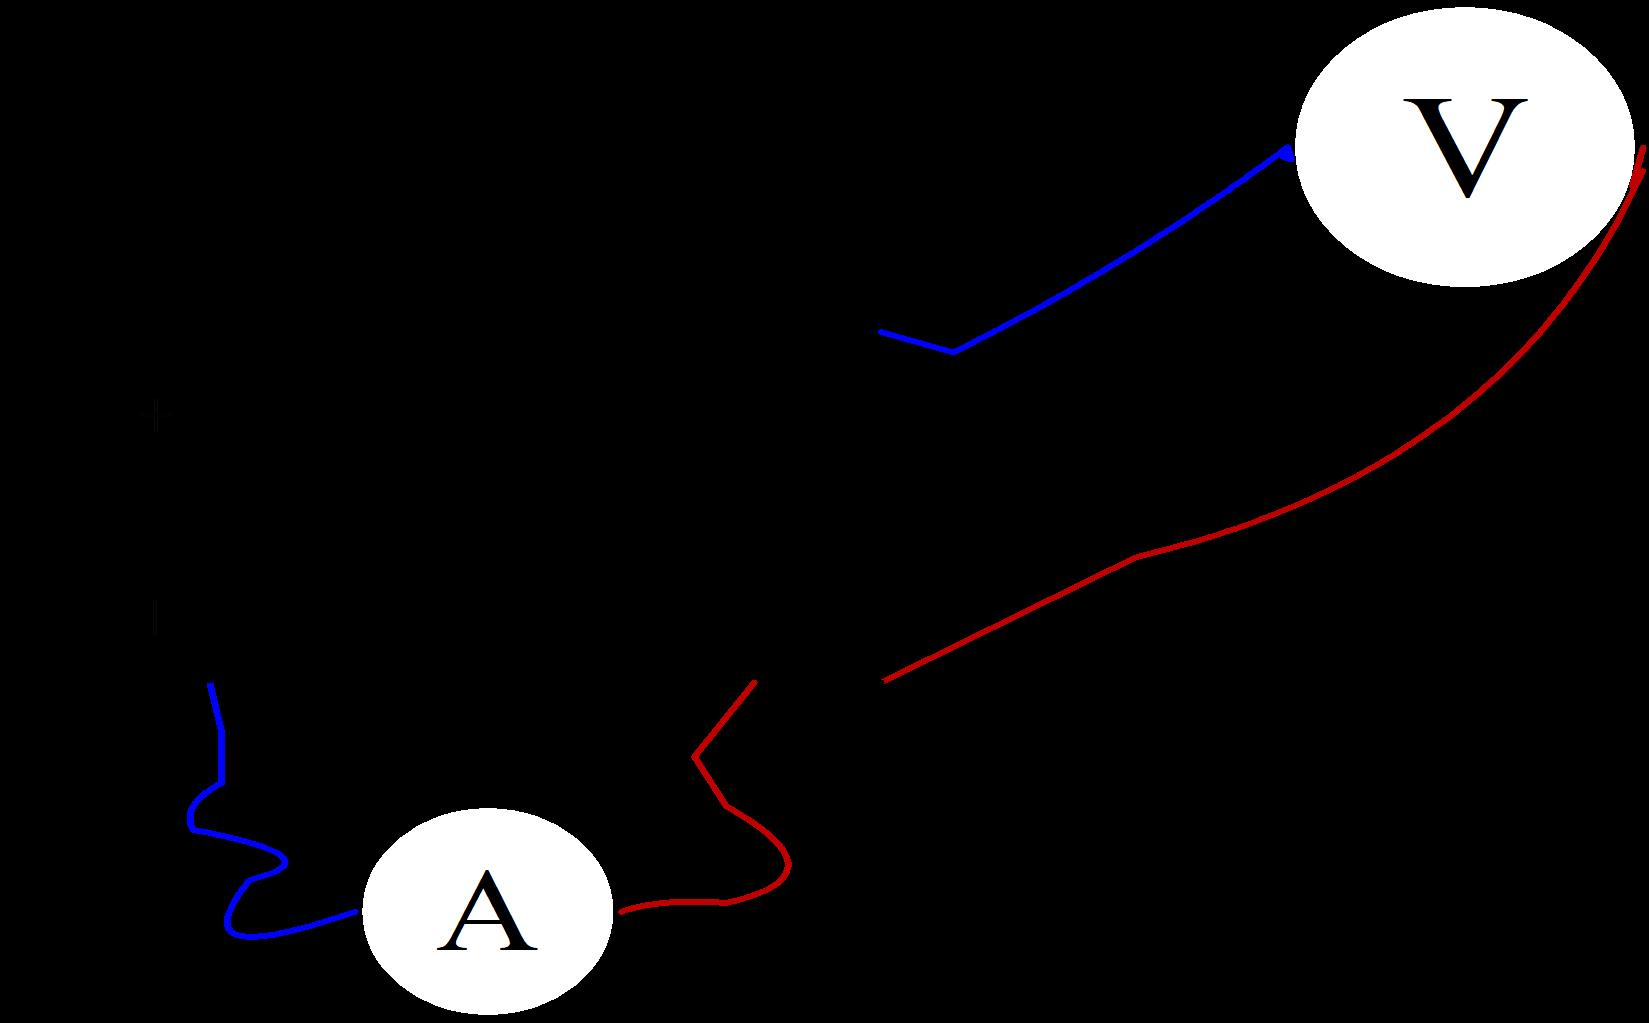
\includegraphics[width=1.9372in,height=1.471in]{PH4CAU18}
\end{figure}

Where a wire was, I have drawn an ammeter. The current must flow through the ammeter for us to measure it.

\begin{figure}[h!]
	\centering
    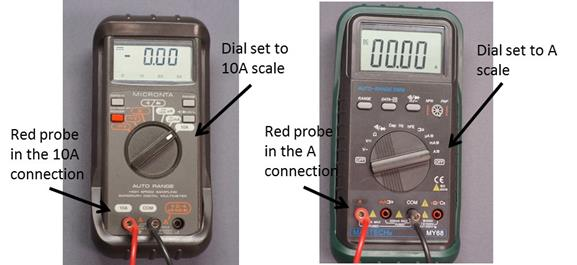
\includegraphics[width=4.858in,height=2.2423in]{PH4CAU19}
\end{figure} 

Remember, to use our multimeters to measure current, we must turn the dial to the $10\unit{A}$ setting AND move the red probe to the $10\unit{A}$ connector. Failure to do this may result in the fuse blowing. Our meter does not warn you that it lost a fuse, it just pays you back by giving really wrong answers. You should be careful to connect it right, and be sure it is working (that someone else has not blown the fuse before you). Since we have different kinds of multimeters, a
second is pictured to the right. For this type of meter, put the red lead in the connector marked $A$ and turn the dial to the $A$ setting. If the currents you are measuring are very small, you might have to switch settings once again. Tiny currents can be measured by moving the dial to the $\unit{mA}$ setting AND changing the red probe to the $\unit{mA}$ connector.

\begin{figure}[h!]
	\centering
    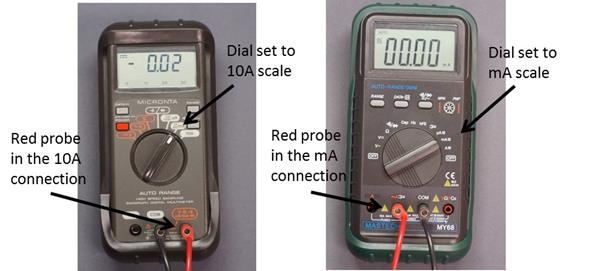
\includegraphics[width=4.9769in,height=2.2928in]{PH4CAU1A}
\end{figure}

Our multimeters really measure current in much the same way we are talking about for our new Arduino ammeter. They have a series of shunt resistors inside of them. When we choose a current measurement setting we are choosing a shunt resistor to put in the circuit (inside the meter, but the meter is in the circuit). Then the voltmeter will measure the voltage across that resistor and use that voltage to calculate the current.

If we create the current meter ourselves, we have to know the resistance that we used! That allows us to use the voltage meter to calculate the current,

\begin{equation*}
	I=\frac{\Delta V_{meter}}{R_{shunt}}
\end{equation*}

but our multimeters are programed to know their own shunt resistances and to do this calculation for us.

If you have time (and some won't) in today's lab, we will build the new Arduino instrument to measure current , and we will test it with a multimeter set in ammeter mode. We will put both in the circuit at the same time (see figure \ref{New Instrument and Test} in the assignment section below) so we get readings from both. Then we can compare and see how well our new instrument works!

\section{Calculating uncertainty, a review}

That is all the new material for today's lab. But I wanted to remind you of
something you already know.

Back in PH150 you should have gotten a good deal of experience in making
measurements. We will be going back to experimentation soon, and we will
need to remember what we learned in PH150 to take the measurements so that
we can interpret our experimental results. You will remember that every
measurement has an uncertainty. We have to estimate that uncertainty. It
turns out that our voltage measurement schemes will introduce a new source
of uncertainty! And we will have to include this in our uncertainty
calculations. We will take that on next lab, but in this lab let's review
how to calculate uncertainties (If you took our PH150 recently, you can skip this section!).

This is a ``review.'' How much of a ``review'' it is may depend on where and when you took PH150 or its equivalent. If you are a chemist, you will note that our treatment of uncertainty goes beyond what you learned in Quantitative Analysis. Let's start by reviewing what a derivative is.

For our purposes, a derivative is a slope of a line. You should recognize the equation of a straight line as

\begin{equation*}
	y=mx+b
\end{equation*}

The slope $m$ can be written as 

\begin{equation*}
	m=\frac{dy}{dx}
\end{equation*}

This is nothing magic (or new). It is just a strange way to write $m.$ With the slope written this way, the equation of the line could be written as 

\begin{equation*}
	y=\frac{dy}{dx}x+b
\end{equation*}

But why $dy/dx$? Think of how we find a slope of a line. Back in junior high
school we called the slope the ``rise over run.'' That is, the change in $y$-value divided by the
change in the $x$-value.

\begin{equation*}
	m=\frac{y_{2}-y_{1}}{x_{2}-x_{1}}
\end{equation*}

In physics, we write the change in a variable using the Greek letter delta, $\Delta .$ So we could write the slope as

\begin{equation*}
	m=\frac{y_{2}-y_{1}}{x_{2}-x_{1}}=\frac{\Delta y}{\Delta x}
\end{equation*}

Just to jog your memory, let me write out $\Delta y$

\begin{equation*}
	\Delta y=y_{2}-y_{1}
\end{equation*}

and $\Delta x.$ 

\begin{equation*}
	\Delta x=x_{2}-x_{1}
\end{equation*}

So our straight line equation should be written 

\begin{equation*}
	y=\frac{\Delta y}{\Delta x}x+b
\end{equation*}

but if we take $\Delta x$ to be very, very small it is customary to write the $\Delta x$ as just $dx$ (I guess a ``$d$'' is smaller than a ``$\Delta $'' ). If this is not familiar from Math 112, is should be by now from PH121.

In PH121 you learned that the velocity is the slope of the plot of $x$ vs. $t,$ for example, 

\begin{equation*}
	y=\frac{1}{2}\frac{\unit{m}}{\unit{s}}t+1\unit{m}
\end{equation*}

is an equation giving the $y$ position of an object as a function of time. Note that it is a straight line on a $y$ vs. $t$ plot. 

\begin{figure}[h!]
	\centering
    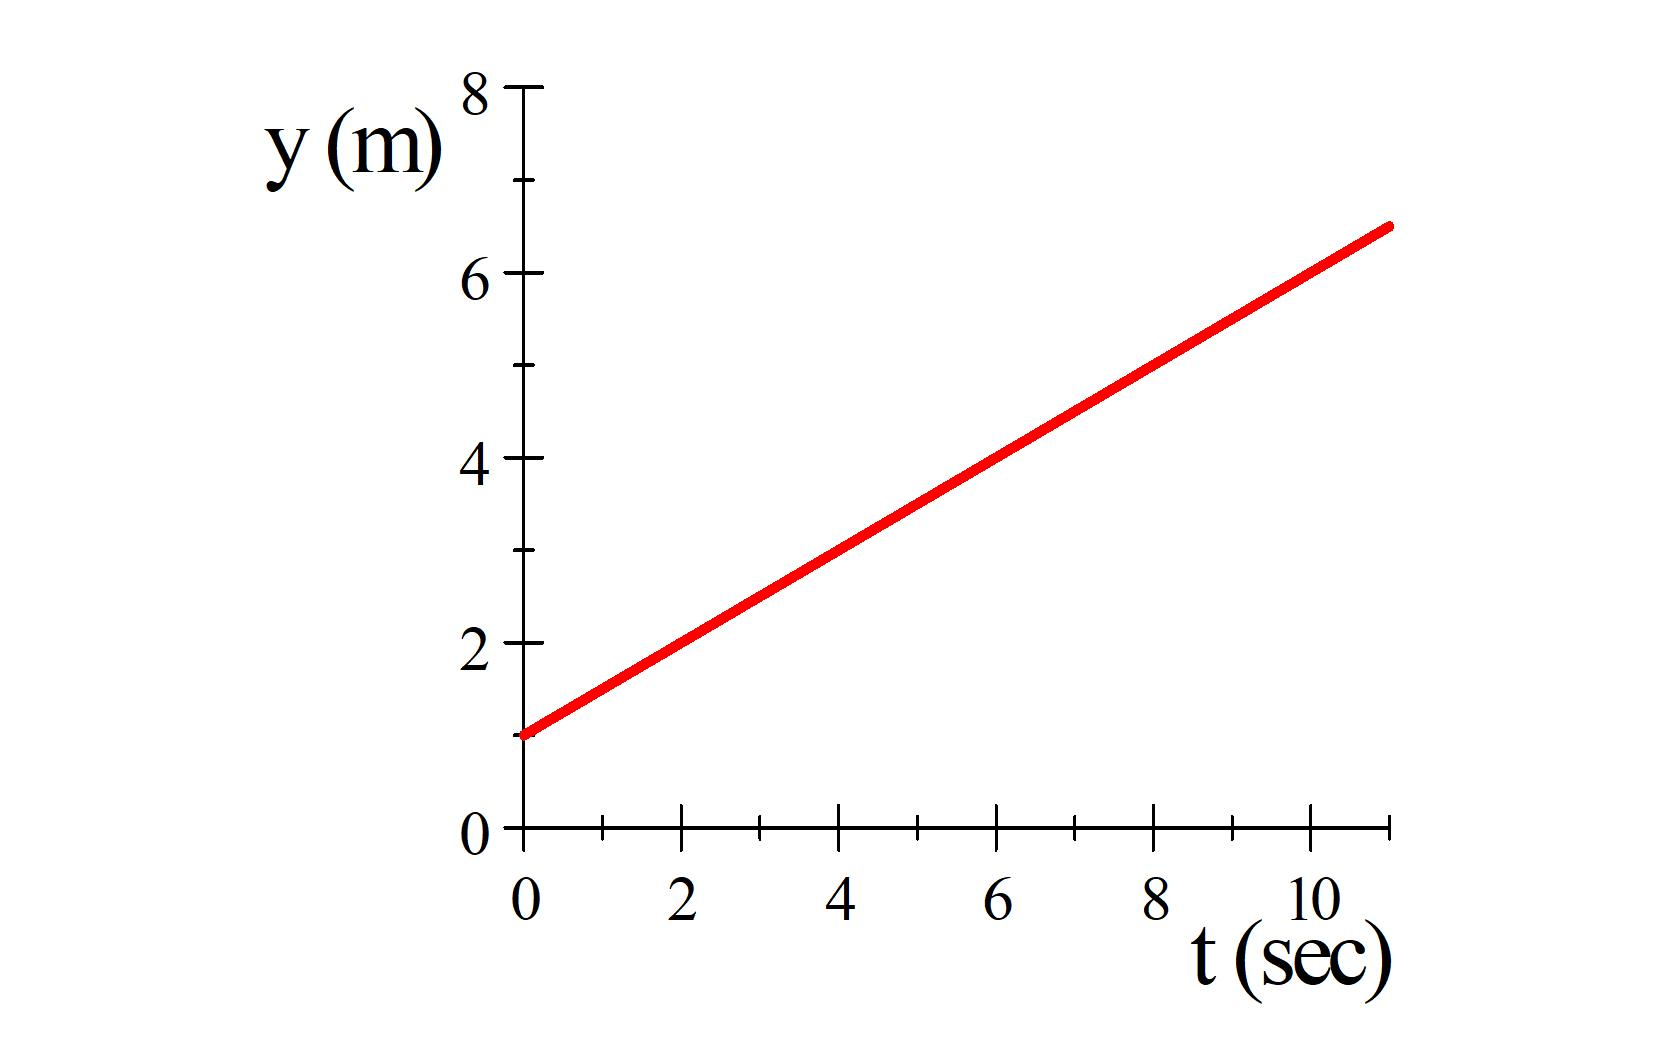
\includegraphics[width=3.3in,height=1.68in]{PH4CAU1B}
\end{figure}

The slope of the line is 

\begin{equation*}
	\frac{dy}{dt}=\frac{1\unit{m}}{2\unit{s}}
\end{equation*}

We can verify that this works by looking at the plot and noting that for every two units of time, we go up one position unit. The slope is $1/2\frac{\unit{m}}{\unit{s}}.$

But not all curves are straight lines. What do we do with curves that, well, curve?

One idea is that we could split up the curve into little line segments, each with its own slope. We can think of $dy/dt$ as an instantaneous slope, a slope of one of the tiny line segments that make up our curve. This is the sort of speed measurement that your speedometer gives. The speed might be different a short time later. But right now the speed is, say, $0.5\unit{m}/ \unit{s}.$

\begin{figure}[h!]
	\centering
    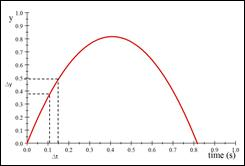
\includegraphics[width=2.8in,height=1.7in]{PH4CAU1C}
\end{figure}

Really, in defining an instantaneous slope we have assumed that the slope near our point on the
curve is essentially a straight line if $\Delta t$ is small enough.

We can use this idea to interpret our error calculations. Suppose I\ throw a ball in the air with a initial speed of $4\unit{m}/\unit{s}$ straight up starting from $y_{o}=0$. From PH121 you have learned that the equation for predicting how high the ball will go is 

\begin{equation*}
	y=y_{o}+v_{o}t+\frac{1}{2}at^{2}
\end{equation*}

It says that starting at $y_{o}$ the ball will go higher depending on the initial velocity, $v_{o},$ and the acceleration, $a.$ That makes sense.

At a time, $t,$ the ball should be at 

\begin{equation*}
	y=0+4\frac{\unit{m}}{\unit{s}}t-\frac{1}{2}\left( 9.8\frac{\unit{m}}{\unit{s}^{2}}\right) t^{2}
\end{equation*}

where $a=-9.8\frac{\unit{m}}{\unit{s}^{2}}$ is the acceleration due to gravity. So, knowing this, I could predict how high the ball would go if I pick a particular time, say, $0.15\unit{s}.$ The result should be

\begin{eqnarray*}
	y &=&0+4\frac{\unit{m}}{\unit{s}}\left( 0.15\unit{s}\right) -\frac{1}{2} \left( 9.8\frac{\unit{m}}{\unit{s}^{2}}\right) \left( 0.15\unit{s}\right) ^{2} \\
      &=&0.489\,75\unit{m}
\end{eqnarray*}

This is shown in the next figure with a black line. Solving the equation for $y$ is equivalent to drawing a line up to the curve, then from our spot on the curve over to the $y$-axis to find the position.

\begin{figure}[h!]
	\centering
    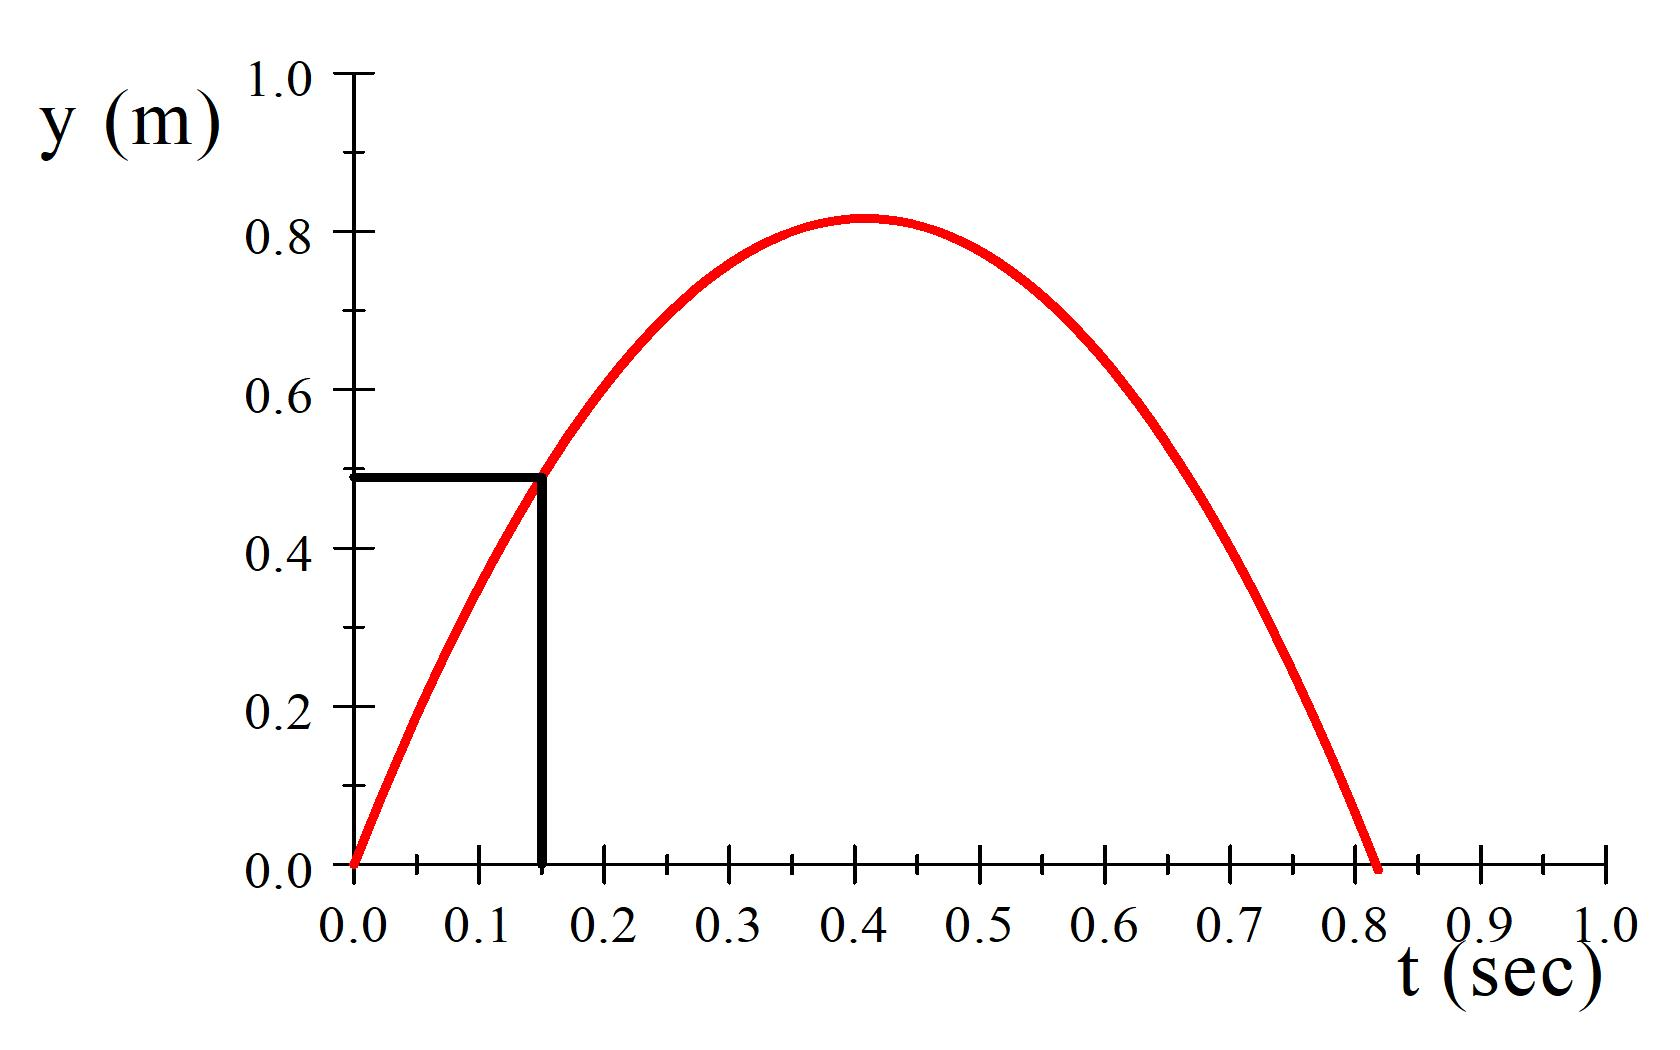
\includegraphics[width=3.3434in,height=2.2295in]{PH4CAU1D}
\end{figure}

For our case, we plot a line upward from $0.15\unit{s}$ to the curve, and then plot a horizontal line from the intersection to the $y$-axis. We can see that we get $4.9\unit{m}.$ Suppose I try to verify this by taking a picture of the ball in flight at $0.015\unit{s},$ but my stop watch is only
good to $\pm 0.005$ seconds. I try to take the picture when the watch is at $0.015\unit{s},$ but I might have taken the picture at $0.01\unit{s}$ or at $0.02\unit{s}$ or anywhere in between. My time has some uncertainty. What does the uncertainty in my stop watch time mean for the uncertainty in my $y$ value?

We can get a good approximation by graphically drawing vertical lines up from $t_{\min }$ and $t_{\max }$ to the curve, and then extending horizontal lines from the intersections to the $y$-axis. This gives us a $y_{\min }$ and $y_{\max }.$ Our actual height could be anywhere in between these. This is a way to view our uncertainty in $y.$

\begin{figure}[h!]
	\centering
    \includegraphics[width=4.1658in,height=2.7769in]{PH4CAU1E}
\end{figure}

We can use this idea to find a general way to calculate uncertainties. We could define $\Delta t=t_{\max }-t_{\min }$. If our $\Delta t$ is small enough (so we can write it just $dt$), the curve is essentially a straight line in the region between $t_{\min }$ and $t_{\max }.$ So if we knew the
slope of that line (the derivative $dy/dt$) we could easily figure out the $y_{\max }$ and $y_{\min }$ points to get our uncertainty range, at least if we stay near our $t_{n}$ part of the curve. Recall that our uncertainty in $y$ is about

\begin{equation*}
	\delta y=\frac{y_{\max }-y_{\min }}{2}=\frac{\Delta y}{2}
\end{equation*}

Remembering that 

\begin{equation*}
	y=\frac{dy}{dt}t+b
\end{equation*}

then 
\begin{eqnarray*}
	\Delta y &=&y_{\max }-y_{\min } \\
			 &=&\frac{dy}{dt}t_{\max }+b-\frac{dy}{dt}t_{\min }-b \\
             &=&\frac{dy}{dt}\Delta t
\end{eqnarray*}

From PH150, you will recognize this as almost the uncertainty in a function of one variable! But even if you don't recognize it, we can show that this is true using our definition of $\delta y$ above. The quantity $\Delta t$ is 

\begin{equation*}
	\Delta t=t_{\max }-t_{\min }
\end{equation*}

so our uncertainty in $t$ would be 

\begin{equation*}
	\delta t=\frac{t_{\max }-t_{\min }}{2}=\frac{\Delta t}{2}
\end{equation*}

then 

\begin{eqnarray*}
	\delta y &=&\frac{y_{\max }-y_{\min }}{2} \\
             &=&\frac{1}{2}\frac{dy}{dt}\Delta t \\
             &=&\frac{dy}{dt}\frac{\Delta t}{2} \\
             &=&\frac{dy}{dt}\delta t
\end{eqnarray*}

so

\begin{equation*}
   \delta y=\frac{dy}{dt}\delta t
\end{equation*}

So our uncertainty in $y$ is just the slope at our point on the curve multiplied by our uncertainty in $t.$

But what if we have more than one variable? Say, we have a function $y(x,z),$ we essentially have a two dimensional slope. Think of a hill, you can go down a hill in more than one direction. So we need slope parts for each direction we can go.

\begin{figure}[h!]
	\centering
    \includegraphics[width=2.3495in,height=1.8133in]{PH4CAU1F}
\end{figure}

\begin{equation*}
   \Delta y=\frac{dy}{dx}x\hat{\imath}+\frac{dy}{dz}z\hat{k}
\end{equation*}

But there is a fix we need to make to this equation that you won't learn for several math classes to come. We want to have a slope in the $x$ and $z$ direction, but we want the slopes to be independent. Think back in PH121 when we did two dimensional motion problems, we split the problem into components. We want to do this for our two dimensional uncertainty! The notation for this is

\begin{equation*}
	\Delta y_{x}=\frac{\partial y}{\partial x}x
\end{equation*}

\begin{equation*}
	\Delta y_{z}=\frac{\partial y}{\partial z}z
\end{equation*}

where 

\begin{equation*}
	\frac{\partial y}{\partial x}
\end{equation*}

means the component of the slope \textbf{just} in the $x$ direction. We take a derivative of the function $y,$ but assume only $x$ is a variable (treat $z$ and all $z$ terms with no $x^{\prime }s$ as constants). This lets us separate the $x$ and $z$ parts. A special, one variable derivative like $\partial y/\partial x$ is called a \emph{partial derivative} because you only take one dimension of the derivative at a time. So, if we wish to find the error in some general function $z\left( x,y\right) $ the error is given by
 
\begin{equation*}
	\delta y=\sqrt{\left( \frac{\partial y}{\partial x}\right) ^{2}\delta x^{2}+\left( \frac{\partial y}{\partial z}\right) ^{2}\delta z^{2}}
\end{equation*}

This looks a lot like our slope equation. What we are doing is to assuming the function $y\left( x,z\right) $ is flat in a small region around the point we are studying. then the function has a slope $\partial y/\partial x$ in the $x$-direction, and $\partial y/\partial z$ in the $y$-direction. Each term like 

\begin{equation*}
	\left( \frac{\partial y}{\partial x}\right) \delta x
\end{equation*}

gives how far off we could be in that direction (the $x$-direction in this case). Remember that we have assumed that $y\left( x,z\right) $ is essentially flat near our point of interest. The square root may be something of a mystery, but remember what you have learned about adding vectors in PH121. We add components of a vector to find the magnitude like this
 
\begin{equation*}
	V=\sqrt{V_{x}^{2}+V_{y}^{2}}
\end{equation*}

This comes from the Pythagorean theorem. The $x$ and $y$ parts of the vector form two sides of a triangle. We want the remaining side. So we use the Pythagorean theorem to find the length of the remaining side.

We are doing the same for our small uncertainty lengths. We are just adding the $x$ and the $y$ components of the error. We could write our error formula for the general case of a function $f$, that depends on $N$ different variables. 

\begin{equation*}
	\delta f=\sqrt{\sum_{i=1}^{N}\left( \frac{\partial f}{\partial x_{i}}\right)^{2}\delta x_{i}^{2}}
\end{equation*}

We will use this formula a lot, so make sure you understand what it means (ask your instructor for help if it is not clear).

\subsection{How do we find the slope?}

But now we have an equation in terms of slope written as $\partial y/\partial x$ or $\partial y/\partial z$, but how would we ever find these slopes? Your calculus class has or will teach you how to take a derivative. They might not have yet taught you how to take this type of derivative. The symbol $\partial $ means that our derivatives are ``partial'' derivatives. This means that we assume all the variables other than the one that shows up in the derivative symbol are constants for our derivative.

Let's take an example. What is the slope of the function $y=5zx^{3}?$ if we calculate the slope only going in the $x$-direction (that is, if we take a partial derivative with respect to $x$) we get

\begin{equation*}
   \frac{\partial }{\partial x}\left( 5zx^{3}\right) =5z\left( 3\right) x^{3-1}=15zx^{2}
\end{equation*}

notice that we treated $z$ as a constant! That is what we mean when we user the symbol $\partial $ and when we say \textquotedblleft partial derivative.\textquotedblright\ Let's try another. How about finding the slope of $f=7yx^{2}-2x+z$ with respect to the $x$-direction.

\begin{equation*}
   \frac{\partial }{\partial x}\left( 7yx^{2}-2x+z\right) =7y\left( 2\right)x^{1}-2(1)x^{0}+z\left( 0\right)
\end{equation*}

The last term illustrates that the slope of a constant is zero, and as we go just in the $x$-direction, $z$ is constant. That makes sense. So the change in $f$ just due to the last term $(z)$ should be zero. We also remember $x^{0}=1.$ So we are left with 

\begin{equation*}
	\frac{\partial }{\partial x}\left( 7yx^{2}-2x+z\right) =14yx-2
\end{equation*}

We could also find 

\begin{equation*}
	\frac{\partial }{\partial y}\left( 7yx^{2}-2x+z\right) =7x^{2}
\end{equation*}

and

\begin{equation*}
	\frac{\partial }{\partial z}\left( 7yx^{2}-2x+z\right) =1
\end{equation*}

In our equation for calculating uncertainties, we want to find the uncertainty in each dimension (for each variable) and to add these uncertainties like components of vectors, so this partial derivative is just what we want, the slope of our function in just one direction.

\subsubsection{Tie to statistics}

Back in PH150 you should have learned that for experiments where we repeat the same experiment over and over again, our outcome can be given by the mean value an our uncertainty can be given by the standard deviation. We need to tie our statistical ideas into what we have learned about error propagation. Lets go back to our function $f\left( x,z\right) $ the error is given by 

\begin{equation*}
	\delta f=\sqrt{\left( \frac{\partial f}{\partial x}\right) ^{2}\delta x^{2}+\left( \frac{\partial f}{\partial z}\right) ^{2}\delta z^{2}}
\end{equation*}

but now we know we could express this in terms of standard deviations (provided you don't need to ensure every bit of your data are within your uncertainty range). We can write our uncertainties as 

\begin{equation*}
	\sigma _{f}=\sqrt{\left( \frac{\partial f}{\partial x}\right) ^{2}\sigma_{x}^{2}+\left( \frac{\partial f}{\partial z}\right) ^{2}\sigma _{z}^{2}}
\end{equation*}

So one way to get an estimate of uncertainty like $\delta x$ or $\delta z$ above is to make many measurements, and use the standard deviation $\sigma_{x}$ as an estimate for $\delta x$ and $\sigma _{z}$ for $\delta z.$ This is usually not too far off (we will refine this analysis in PH336 for those lucky enough to take the course).

We can use connection between $\delta x$ and $\sigma _{x}$ to show that the standard deviation of the mean (the best estimate of our uncertainty) is given by

\begin{equation*}
	\sigma _{\bar{x}}=\frac{\sigma _{x}}{\sqrt{N}}
\end{equation*}

(a result you should have learned back in PH150). Think of calculating a mean value

\begin{equation*}
	\bar{x}=\frac{x_{1}+x_{2}+\cdots x_{N}}{N}
\end{equation*}

We can find the uncertainty in this function $\sigma _{\bar{x}}$

\begin{equation*}
	\sigma _{\bar{x}}=\sqrt{\left( \frac{\partial \bar{x}}{\partial x_{1}} \right) ^{2}\sigma _{x_{1}}^{2}+\left( \frac{\partial \bar{x}}{\partial x_{2}}\right) ^{2}\sigma _{x_{2}}^{2}+\cdots +\left( \frac{\partial \bar{x}}{\partial x_{N}}\right) ^{2}\sigma _{x_{N}}^{2}}
\end{equation*}

You see we just take the partial derivative of our function $\bar{x}$ with respect to each of the variables $x_{i}$ and multiply by the uncertainty in that variable written now as a standard deviation $\sigma _{i}.$

For this special case, all of the $x_{i}$ are the same (we are measuring the same value over and over in taking an average) and all of the $\sigma _{i}$ are the same so we just have

\begin{equation*}
	\sigma _{\bar{x}}=\sqrt{N\left( \frac{\partial \bar{x}}{\partial x_{1}} \right) ^{2}\sigma _{x_{1}}^{2}}
\end{equation*}

and we can take the derivative using our rule. Only $x_{1}$ is a variable, so we can write the average $\bar{x}$ as 

\begin{equation*}
	\bar{x}=\frac{x_{1}}{N}+\frac{x_{2}+\cdots x_{N}}{N}
\end{equation*}

This is a polynomial! The first term is $\frac{1}{N}x_{1}$ and the whole second term is a constant if we take a partial derivative with respect to $x_{1}$. The derivative is 

\begin{eqnarray*}
	\frac{\partial \bar{x}}{\partial x_{1}} &=&\frac{\partial }{\partial x_{1}}\left( \frac{x_{1}}{N}+\frac{x_{2}+\cdots x_{N}}{N}\right) \\
                                            &=&\frac{1}{N}x_{1}^{0}+0 \\
                                            &=&\frac{1}{N}
\end{eqnarray*}
so our statistical error function is just 

\begin{eqnarray*}
	\sigma _{\bar{x}} &=&\sqrt{N\left( \frac{1}{N}\right) ^{2}\sigma _{x_{1}}^{2}} \\
                      &=&\sqrt{\frac{\sigma _{x_{1}}^{2}}{N}} \\
                      &=&\frac{\sigma _{x_{1}}}{\sqrt{N}}
\end{eqnarray*}

or, since all the $\sigma _{x_{i}}$ are the same, we can just write this as 

\begin{equation*}
	\sigma _{\bar{x}}=\frac{\sigma _{x}}{\sqrt{N}}
\end{equation*}

Notice that in this example we had many $x_{i}$ and that to find the uncertainty we just extended our equation from two variables

\begin{equation*}
	\sigma _{f}=\sqrt{\left( \frac{\partial f}{\partial x}\right) ^{2}\sigma_{x}^{2}+\left( \frac{\partial f}{\partial z}\right) ^{2}\sigma _{z}^{2}}
\end{equation*}

to $N$ variables

\begin{equation*}
	\sigma _{f}=\sqrt{\sum_{i=1}^{N}\left( \frac{\partial f}{\partial x_{i}}\right) ^{2}\sigma _{i}^{2}}
\end{equation*}

In this special case, we were trying to show a special result, but we can do this for any function with any number of variables. If your function is complicated, you just need to take more partial derivative terms under the square root.

I'm sure you remembered all of that from PH150. But now it is time to move on to today's lab assignment.
\vfill
\pagebreak
\section{Practice Measurements}
Here are some measurements to try with the instruments we learned about in this reading.

\subsection{Use a Multimeter}

\begin{enumerate}
\item Measure the voltage of a D-Cell battery with a voltmeter. Report the value you get from the measurement and the uncertainty.

\item Set up the circuit described in section (\ref{Voltage Measurement with Meter}). The figure is repeated below. Measure the voltage with a multimeter. \textbf{The indicator on the power supply is not very accurate}, but it can serve as a check to see if we are way off. So compare the power
supply voltage indicator to the meter indicator. Are they the same (you should think of the uncertainty in both meters and answer using the uncertainties)

\begin{figure}[h!]
	\centering
    \includegraphics[width=4in,height=2in]{PH4CAU1G}  
\end{figure}

\item Modify your circuit described in section (\ref{Voltage Measurement with Meter}) and change the settings of your multimeter so that you measure the current in the circuit. Compare your ammeter measurement to the current shown on the power supply indicator.
\end{enumerate}

\subsection{Use an Oscilloscope}

\begin{enumerate}
\item Predict what you will see on an oscilloscope if you measure the voltage of a D-Cell battery. Make sure your lab table agrees on your prediction before you go on.

\item Use the oscilloscope to measure the voltage of a D-Cell battery.

\item Practice interpreting oscilloscope screens

\begin{enumerate}
\item Figure out what the markings on the Oscilloscope screen mean.

\item Figure out what the voltage scale is and how to change it

\item Figure out what the time scale is and how to change it
\end{enumerate}

\item Generate a sinusoidal signal using the stand alone Signal Generator.

\item Measure and display this signal using the stand alone digital
oscilloscope.

\item Report the amplitude and the frequency (and their uncertainties) of
the measured signal and compare to the signal generator settings.
\end{enumerate}

\subsection{Build a new instrument from an old instrument}

\begin{enumerate}
\item IF\ THERE\ IS\ TIME, choose a resistor in the $20\unit{k\Omega}$ range (say, from about $10\unit{k\Omega}$ to about $30\unit{k\Omega}$). Choose a shunt resistor in the $200\unit{\Omega}$ range. Then set up the circuit to measure a current. 

\begin{figure}[h!]
	\centering
    \includegraphics[width=3.8744in,height=3.0874in]{PH4CAU1H}
    \label{New Instrument and Test}
\end{figure}

Use an additional multimeter set to measure current to check our
voltage-current measurement. Calculate a percent difference to see how well
this worked.
\end{enumerate}


\vspace*{\fill}
\pagebreak
	
	%\chapter{First DAQ Measurements: Voltage}
		%DAQ_Measuremnt_V
\chapter{First DAQ Measurements: Voltage}
Let's review what we learned last week. In physics equipment, we try to
measure voltages. If your data is not a voltage, we try to convert it into a
voltage. Already we converted current into a voltage (using a shunt
resistor). But what is a voltage? We said last week that it is a measure of
electrical potential energy. It is also likely that you know the word
\textquotedblleft voltage\textquotedblright\ because we live in a world that
has electricity everywhere. You probably know that your house or apartment
has wires in the walls that carry \textquotedblleft 110
Volts.\textquotedblright\ And you probably realize that \textquotedblleft
voltage\textquotedblright\ is a measure of how much energy there is in the
wires.

Soon your PH220 class will explain that \textquotedblleft
voltage\textquotedblright\ is proportional to the electrical potential
energy difference. But for us, now, we just need to know that we are
measuring something proportional to energy and we need to learn how to
measure it.

\begin{figure}[h!]
	\centering
	\includegraphics[width=2.8in,height=2.5in]{PH4CAU1I}
\end{figure}

Because voltage is proportional to a \emph{difference} in electrical
potential energy, a voltage measurement really is a combination of two
measurements. Think of gravitational potential energy. If we ask for the
potential energy difference as Super Guy jumps from the bottom of a building
to the top we need two measurements, one at the bottom and one at the top. Then 

\begin{equation*}
	\Delta U_{g}=U_{g_{top}}-U_{g_{bottom}}
\end{equation*}

We will do something very similar in measuring voltages. We will measure the
potential energy at two places. For example, suppose we have an electric
circuit as shown in the next figure. 
\begin{figure}[h!]
	\centering	
    \includegraphics[width=3.5466in,height=1.3932in]{PH4CAU1J}
\end{figure}
The circuit is very simple, just a battery and a resistor. You have experience with batteries, and resistors now. A resistor is just a piece of material that has lots of electrical friction, or \textquotedblleft resistance\textquotedblright\ that makes it
hard for electrons to go through it. If we want to measure the voltage across the resistor, we have to measure on the top and bottom of the resistor. That will give us a measurement proportional to the potential energy difference from one side to the other of the resistor.

Most meters that measure voltage have two \textquotedblleft
probes\textquotedblright\ and do the difference calculation internally.
These meters are called \emph{voltmeters} and we used them last week.

\begin{figure}[h!]
	\centering
	\includegraphics[width=2.9199in,height=1.962in]{PH4CAU1K}
\end{figure}

In today's world, voltmeters are usually just one part of a device that can
measure many things. We call these devices multimeters. To measure voltage
we will set the multimeter on the DC Voltage setting. Notice the two probe
wires in the figure. We need two probes to make the two measurements and the
device does the subtraction for us.

We learned to use a sand-alone voltmeter in the last lab. But we also need
to read in voltages in a way that the data shows up on our computer. To get
the data into our computer we will use a different set of pins on our
Arduino board. They are called \emph{analog} pins.

Even before we begin, we need a warning. We absolutely must not wire up the
analog pins on our Arduino backwards! This can (and probably will) destroy
the pin circuitry inside our Arduino. So we will need to be careful in
wiring for this part of our lab. Where this could be a problem a warning
sign will appear in the text, just to remind you to be careful! 

\begin{figure}[h!]
	\centering
	\includegraphics[width=2.8089in,height=1.4684in]{PH4CAU1L}
\end{figure}

You may see quite a few of these in this lab.

\section{Building a voltmeter}

Our Arduino has what we call and Analog to Digital converter (ADC). That is,
it takes analog voltage signals that could have any value, and it maps them
into a set of discrete values and sort of rounds to the nearest whole
discrete value.

The word ``analog'' might not be familiar.
Think of our power supply. It has a knob that adjusts the voltage. The knob
can produce any voltage from $0$ to about $30\unit{V}$. This is an analog
signal. The voltage can take on any value in a range. So we represent an
analog signal with real numbers and we might have a voltage of exactly 

\begin{equation*}
	4.3276854325532573457\unit{V}
\end{equation*}

and this would be perfectly valid for an analog signal.

A battery, on the other hand, is not this way. It has a fixed voltage, say, $1.5\unit{V}$ like the D-Cell batteries that we used in our last lab. Two D-Cell batteries could be used together to make $3\unit{V}.$ But you can't use D-Cell batteries to get $2.25\unit{V}.$ The batteries come in discrete units.

Our Arduino analog pin is designed to measure voltages in the range $0$ to $5\unit{V}.$ Don't set your power supply to more than $5\unit{V}!$ But there is more to the ADC than just a voltage range. The Arduino chops the voltage range into 1024 discrete voltage divisions. Each division is then

\begin{equation*}
	\Delta v_{\min }=\frac{5\unit{V}}{1024}=4.\,\allowbreak 9\unit{mV}
\end{equation*}

\begin{figure}[h!]
	\centering
	\includegraphics[width=2.3618in,height=1.5714in]{PH4CAU1M}
\end{figure} 

This means that changes in
voltage that are less than $4.9\unit{mV}$ won't be seen, since it takes a whole $4.9\unit{mV}$ to get a different division. So if we give our Arduino $8\unit{mV}$ this is not enough to fill the second $4.9\unit{mV}$ division, so our Arduino would still read only $4.9\unit{mV}.$ If we gave it $11\unit{mV}$ it would then read $9.8\unit{mV}$ because $9.8\unit{mV}=2\times 4.9 \unit{mV}$ and $9.8$ is the closest whole unit of $4.9\unit{mV}.$

\begin{figure}[h!]
    \centering
    \includegraphics[width=3.1868in,height=2.9265in]{PH4CAU1N}
\end{figure}

This is called ``discretization'' or more commonly ``digitization'' or even \emph{``quantization.'' } We have taken a signal that might have any value between $0$ to $5\unit{V}$ and we output a signal that will be rounded to the nearest $n\times 4.9\unit{mV}.$

As a second example, $3.793\unit{V}$ would be reported as $\allowbreak 3.792\,\allowbreak 6\unit{V}$ since 

\begin{equation*}
	\frac{3.793\unit{V}}{4.9\unit{mV}}=774.\,\allowbreak 08
\end{equation*}

but we need even units of $\Delta v_{\min },$ so the $0.8$ would be dropped by the A2D converter giving 

\begin{equation*}
	774\times 4.9\unit{mV}=\allowbreak 3.792\,\allowbreak 6\unit{V}
\end{equation*}

and our first voltage from our power supply, $4.3276854325532573457\unit{V}$
would be reported as $4.\,\allowbreak 326\,7\unit{V}$ (make sure you can see
how we got this result!).

This means that we can be off in our voltage measurements as much as $4.9%
\unit{mV}$! In dividing up our voltage range into $1024$ pieces we have
introduced some error, but we have divided our $0$ to $5\unit{V}$ into
numeric values that we can use in our computer, so it is worth the cost of
some error.

The amount of error depends on how many different values the ADC converter
has. Since breaking an analog signal into discrete values is called \emph{
quantization, }we call this source of error \emph{quantization error.} It is
the source of much of the error we see in electronic measuring devices. We
could say that our new voltmeter has an uncertainty of at least the voltage
resolution

\begin{equation*}
	\delta V_{signal}=\Delta V_{\min }=4.\,\allowbreak 9\unit{mV}
\end{equation*}

but of course it could be larger if there are other sources of error.

The ADC sends the measured value through our USB cable to our computer's
serial port. But it doesn't send it in units of volts. It sends it in ADC
units. If we have a signal voltage of $9.8\unit{mV}$ we don't get out $9.8,$
we get $2$ because $9.8\unit{mV}=2\Delta V_{\min }.$ The ADC units are the
number of $\Delta V_{\min }$ sized units that are in our signal voltage. To
get back to voltage units, we need to multiply by $\Delta V_{\min }.$ In our
code we will do this before reporting the value.

Of course we would like to see the voltage that we measure. There is a
simple way to do this. The voltage values we calculate can be sent to our
computer through the serial cable. We will need an Arduino sketch with some
additional setup and some additional loop commands. One of these commands
will turn our ADC units into volts.

Before we look at the entire sketch, let me introduce the new commands that
we will need. To get the Arduino to communicate with the computer we use the
command 
\begin{equation*}
	\begin{tabular}{l}
		\ Serial.begin();
	\end{tabular}%
\end{equation*}
and in the loop function we use the command\ 
\begin{equation*}
	\begin{tabular}{l}
		\ Serial.print();
	\end{tabular}%
\end{equation*}

We also need to know that computers make a distinction between integer and
real numbers. Our voltages will be real numbers, so we need to tell the
Arduino that we want a real number. The command for this is the word
\textquotedblleft float.\textquotedblright\ For example,

\begin{equation*}
	\begin{tabular}{l}
		\ float\ delta\_v\_min=0.0049;
	\end{tabular}
\end{equation*}

defines a variable named ``delta\_v\_min'' and sets it to the value $0.0049.$ If we want an integer number we use the word ``int.'' For example

\begin{equation*}
	\begin{tabular}{l}
		\ int\ value\ =\ 0;
	\end{tabular}
\end{equation*}

defines a variable named ``value'' and sets it equal to $0.$ All this is a little like listing your variables back in PH121. Only here if you don't do it, it doesn't just cost you points, it confuses the Arduino software and the Arduino software will give you an error.

We also need special commands to read our Arduino analog pins. The special Arduino command 

\begin{equation*}
	\begin{tabular}{l}
		analogRead()
	\end{tabular}
\end{equation*}
will do this.

The whole Arduino sketch might look like this:
\href{https://dtoliphant.github.io/PH250Manual/Code/DAQ_voltmeter.ino}{Download here}
\lstinputlisting[language=Arduino]{Code/DAQ_voltmeter.ino}


Make sure you understand every line of this code. Write it in the Arduino IDE and run it to help see what the lines do. Lines that begin with two slashes, ``//,'' are comments. The Arduino will ignore these lines. But you shouldn't! The comments tell you, the programmer, what the code is doing. I will ask you in lab to input comments
for every line. If there is any part of this sketch that is mysterious, work with your group to resolve the mystery and if it is still mysterious, call your instructor over to discuss the sketch with you.

\subsection{Wiring the simple voltmeter}

\begin{figure}[h!]
	\centering
	\includegraphics[width=1.8507in,height=0.9677in]{PH4CAU1O}
\end{figure}
You knew that was coming, didn't you! We must be very careful to wire our Arduino correctly. Our Arduino can measure $0$ to $5\unit{V}.$ But if we switch the $5\unit{V}$ and the $0\unit{V}$ by plugging them into the wrong pin, our Arduino may be damaged and never work the same way again (probably won't work at all!). So wire
first, then before you connect the Arduino have group member check your wiring, then check the wiring with a stand-alone meter (that is why we learned to use them last week). Also remember, more than $5\unit{V}$ will damage the Arduino. So only put in voltages in the range $0\unit{V}$ to $5 \unit{V}.$

We need one wire attached to the pin marked A0. We need another wire
attached to one of our Arduino ground pins marked GND. And we connect the
first wire to the positive output of our signal source (say, our power
supply) and the GND wire to our negative output of our signal source (say
the negative or ground connection on our power supply). That is all there is
to it!

\subsection{Seeing the data}

Once the code is compiled and uploaded, the Arduino will send data to the
serial port. The serial monitor can display the data. The serial monitor is
found under the Arduino Software Tools menu.

\begin{figure}[h!]
	\centering
	\includegraphics[width=2.0807in,height=3.0744in]{PH4CAU1P}
\end{figure}
You should see something like this:

\begin{figure}[h!]
	\centering
	\includegraphics[width=4.5861in,height=2.3151in]{PH4CAU1Q}
\end{figure}

The Arduino Software can also plot the data from the serial port. Here is a
plot of the same data that we saw on the serial monitor. 

\begin{figure}[h!]
	\centering
	\includegraphics[width=3.563in,height=1.8049in]{PH4CAU1R}
\end{figure}
Notice that it plotted our voltage values and it also plotted our ADC values. This makes the voltage values hard to see. We could fix this by commenting out the lines that print the ADC values (putting \textquotedblleft //\textquotedblright\ at the
beginning of the line). Then those lines won't be executed by the Arduino.
Then we get just the voltage. 

\begin{figure}[h!]
	\centering
    \includegraphics[width=3.2578in,height=1.6475in]{PH4CAU1S}
\end{figure}

Notice that the horizontal axis is not exactly time. It is just the data point number. We could convert this to time with some calculation if we know how often the Arduino sends us a data point. I will leave this as an exercise.

\section{Extending our voltmeter with a voltage divider\label{Voltmeter with
Voltage Divider}}

This Arduino-based voltmeter that we have built is great, but will only let
us measure voltages in the range $0$ to $5\unit{V}.$ That seems a little
restrictive. We would like to extend our voltmeter to a larger range, say, $%
0 $ to $20\unit{V}.$ To do this, we will need to add some electronic
components and think about what we have learned about voltage, resistance,
and current. Let's consider this circuit.

\begin{figure}[h!]
	\centering
	\includegraphics[width=1.3932in,height=1.3188in]{PH4CAU1T}
\end{figure}

We have a battery, That will make the current flow much like a pump makes water move through pipes.

\begin{figure}[h!]
	\centering
	\includegraphics[width=4.2004in,height=2.3229in]{PH4CAU1U}
\end{figure}

The water in a pipe system gains potential energy as it moves up. In our circuit we will find that electric charge gains potential energy as we move it across a battery. Then the charge will move down the wire like water moves down a pipe until it is out
of potential energy. Notice that the water in a pipe system will lose all the potential energy that it gained when the pump raised it to the upper tank (see previous figure). That is true of electric charge too. The electric current travels from the battery through the resistor, but in doing so it loses all the potential energy that the battery gave it by the time it returns to the battery.

Now suppose we have two resistors in a circuit.

\begin{figure}[h!]
	\centering
	\includegraphics[width=1.7279in,height=1.5947in]{PH4CAU1V}
\end{figure}

Our water analogy can still help us understand what will happen. Suppose
that we have two turbines in our pipe system. 

\begin{figure}[h!]
	\centering
	\includegraphics[width=3.5985in,height=1.9934in]{PH4CAU1W}
\end{figure}

The water leaves the high potential energy part of the pump, and is put to work turning the first turbine. The resistance of the turbine will slow the water current. So when the water leaves the turbine, it will have lost some potential energy. Since
we have a second turbine the current will again be slowed and more potential
energy will be lost. How much potential energy do we lose as the water
falls? All of the potential energy that the pump gave it! We must end up
with the water at the bottom back at the low potential energy. We will find
this to be true for our electric circuit as well. We will loose some
potential energy as the electrical energy \textquotedblleft
falls\textquotedblright\ from the high electric potential \textquotedblleft
down\textquotedblright\ the first resistor. After the second resistor, we
can guess that we must be back at the low electric potential we started with.

\begin{figure}[h!]
	\centering
	\includegraphics[width=1.7279in,height=1.5947in]{PH4CAU1X}
\end{figure}

We know that electric potential is a potential energy per unit charge. And energies just add up. If 

\begin{equation*}
	\Delta V=RI
\end{equation*}

is satisfied, then we would expect that adding two resistors would just linearly add the effects of the two resistors together

\begin{eqnarray*}
	\Delta V_{total} &=&\Delta V_{1}+\Delta V_{2} \\
	&=&R_{1}I+R_{2}I
\end{eqnarray*}

Note that the same current must flow through each of the resistors, since the current leaving $R_{1}$ is the current flowing into $R_{2}.$ Then 

\begin{equation*}
	\Delta V_{total}=\left( R_{1}+R_{2}\right) I
\end{equation*}

Our current will be 

\begin{equation*}
	I=\frac{\Delta V_{total}}{R_{1}+R_{2}}
\end{equation*}

But suppose we measure the potential change across just resistor $R_{2}.$ 

\begin{figure}[h!]
	\centering
	\includegraphics[width=1.7625in,height=1.0421in]{PH4CAU1Y}
\end{figure}

what would we expect to get? We lost voltage across both $\Delta V_{1}$ and $\Delta V_{2}$ so 

\begin{equation*}
	\Delta V_{total}=\Delta V_{1}+\Delta V_{2}
\end{equation*}

because we must loose all the $\Delta V_{total}$ given to the current by the
battery. And 

\begin{equation*}
	\Delta V_{2}=IR_{2}
\end{equation*}

from Ohm's law. So

\begin{equation*}
	\Delta V_{2}=\left( \frac{\Delta V_{total}}{R_{1}+R_{2}}\right) R_{2}
\end{equation*}

This is only part of the total voltage. And if we have two different
resistors so that $R_{1}\neq R_{2}$ then we can choose for $\Delta V_{2}$ to
be nearly as much as $\Delta V_{total}$ or nearly as little as $0$ by
carefully choosing our two resistances. We call a set of two resistors like
this a \textquotedblleft voltage divider\textquotedblright\ because it
divides the battery voltage between the two resistors. If $R_{1}$ is bigger
than $R_{2}$ then $\Delta V_{1}$ is bigger than $\Delta V_{2}.$

Remember that the input can only withstand $0$ to $5\unit{V}.$ More than
that can destroy the board! But we want to measure a voltage that varies
from $0$ to $20\unit{V}.$ We now have a way to do this. We will use a
voltage divider. The voltage across both resistors will be as much as $20%
\unit{V},$ but we will measure the voltage across only one of the resistors.
And we will choose our resistor so that when the total voltage is $20\unit{V}
$ but the voltage across our resistor is $5\unit{V}$ (or less). Since we
will know the resistances, we can use a little math to calculate what the
total voltage was using the voltage measurement from just one of the
resistors.

This is like what we did to measure current last lab. We used a voltmeter
and a resistor and some math to make an ammeter. Today we will use two
resistors, our Arduino voltmeter, and some math to make a new voltmeter that
can measure higher voltages. We just need to choose our resistors so that we
map our $0$ to $20\unit{V}$ to $0$ to $5\unit{V}.$ Once choice might be 

\begin{eqnarray*}
	R_{1} &=&40\unit{k \Omega} \\
	R_{2} &=&10\unit{k \Omega}
\end{eqnarray*}

Let's try it. We would get

\begin{eqnarray*}
	\Delta V_{2\max } &=&\left( \frac{20\unit{V}}{40\unit{k \Omega }
	+10\unit{k \Omega }}\right) \left( 10\unit{k \Omega }\right) \\
	&=&4.0\unit{V}
\end{eqnarray*}

when $\Delta V_{total}=20\unit{V}$ and 

\begin{eqnarray*}
\Delta V_{2\min } &=&\left( \frac{0\unit{V}}{40\unit{k \Omega}
	+10\unit{k\Omega}}\right) \left( 10\unit{k\Omega}\right) \\
	&=&0\unit{V}
\end{eqnarray*}

when $\Delta V_{total}=0\unit{V}.$ Notice that this really didn't work. We
only got a maximum voltage of $4\unit{V}.$ But this gives us a margin of
safety. If we give our Arduino more than $5\unit{V}$ we can burn it up. If
we plan our circuit so we don't get to close to $5\unit{V}$ we are safer. So
this set of resisters is not a terrible choice.

To report out our voltage we need to do this conversion backwards. Say we
have $\Delta V_{total}=10\unit{V}$ that we are measuring with our new
instrument. Then 

\begin{eqnarray*}
	\Delta V_{2} &=&\left( \frac{10\unit{V}}{40\unit{k \Omega}
	+10\unit{k\Omega}}\right) \left( 10\unit{k\Omega}\right) \\
	&=&2\unit{V}
\end{eqnarray*}

The $2\unit{V}$ is what we actually measure at the A0 input. But we know
that this represents $10\unit{V}$ across both resistors, so we want the
Arduino program to print out $10\unit{V}.$ So we report%
\begin{equation*}
\Delta V_{reported}=\frac{\Delta V_{2}}{R_{2}}\left( R_{1}+R_{2}\right)
\end{equation*}%
or for our case, since we measured $2\unit{V}$ across our resistor,%
\begin{equation*}
10\unit{V}=\frac{2\unit{V}}{\left( 10\unit{k%
%TCIMACRO{\U{3a9}}%
%BeginExpansion
\Omega%
%EndExpansion
}\right) }\left( 40\unit{k%
%TCIMACRO{\U{3a9}}%
%BeginExpansion
\Omega%
%EndExpansion
}+10\unit{k%
%TCIMACRO{\U{3a9}}%
%BeginExpansion
\Omega%
%EndExpansion
}\right)
\end{equation*}%
We will have to write this math in our code. There is a further
complication. The Arduino A0 input is giving us a number that represents $0$
to $4\unit{V}$ for our setup. But that is not what we see on the serial
port. We see a number from 0 to 1024. We know the $1024$ represents $5\unit{V%
}$ and the $0$ represents $0\unit{V}.$ So we need to multiply the number
that comes from our Arduino by $\delta V=4.9\unit{mV}$ once again to get our
Arduino output into voltage units. So our reported voltage equation is
something like this. 
\begin{equation*}
\Delta V_{reported}=A2D\times \delta V_{2}\times \frac{1}{R_{2}}\left(
R_{1}+R_{2}\right)
\end{equation*}

All this calculation to get our reported voltage must do something to our
measurement uncertainty. We could do our usual math to find the reported
uncertainty, but instead, let's think. Every small voltage $\Delta V_{2}$
would be multiplied by $\left( \frac{1}{R_{2}}\left( R_{1}+R_{2}\right)
\right) $ to map it into our original $0\unit{V}$ to $20\unit{V}$ range.
That should work for our smallest voltage that we can detect, namely $\delta
V=4.9\unit{mV}.$ That is the smallest value $\Delta V_{2}$ could have. So in
our $0\unit{V}$ to $20\unit{V}$ range the smallest value this can map to is 
\begin{equation*}
\delta V_{reported}=\left( \delta V\right) \left( \frac{1}{R_{2}}\left(
R_{1}+R_{2}\right) \right)
\end{equation*}%
The first term in parenthesis is essentially $1$ digitizer unit multiplied
by $\Delta V_{2}$ and the second term in parenthesis converts the $\Delta
V_{2}$ value into actual volts measured across both resistors.

The quantity $\delta V_{reported}$ gives us our quantization error value for
our new instrument. Our output will be in multiples of 
\begin{equation*}
V_{reported}=n\times \delta V_{reported}
\end{equation*}%
Putting in numbers gives 
\begin{eqnarray*}
\delta V_{reported} &=&\left( 4.\,\allowbreak 884\times 10^{-3}\unit{V}%
\right) \left( \frac{1}{10\unit{k%
%TCIMACRO{\U{3a9}}%
%BeginExpansion
\Omega%
%EndExpansion
}}\left( 40\unit{k%
%TCIMACRO{\U{3a9}}%
%BeginExpansion
\Omega%
%EndExpansion
}+10\unit{k%
%TCIMACRO{\U{3a9}}%
%BeginExpansion
\Omega%
%EndExpansion
}\right) \right) \\
&=&0.024\,42\unit{V} \\
&=&24.42\unit{mV}
\end{eqnarray*}%
This is much bigger than our $4.9\unit{mV}$ uncertainty for the simple
voltmeter. And this is the cost of using a voltage divider to extend our
voltage range. For the bigger voltage range we get a bigger uncertainty.

Let's try another example. Suppose we wish to measure $0$ to $20\unit{V}$
and we look in our case of resistors and find we have the following two
resistors to use:%
\begin{eqnarray*}
R_{1} &=&98\unit{k%
%TCIMACRO{\U{3a9}}%
%BeginExpansion
\Omega%
%EndExpansion
} \\
R_{2} &=&15\unit{k%
%TCIMACRO{\U{3a9}}%
%BeginExpansion
\Omega%
%EndExpansion
}
\end{eqnarray*}

We would expect that our $0$ to $20\unit{V}$ would be mapped to a smaller
range. Let's find that range.%
\begin{eqnarray*}
\Delta V_{2\max } &=&\left( \frac{20\unit{V}}{98\unit{k%
%TCIMACRO{\U{3a9}}%
%BeginExpansion
\Omega%
%EndExpansion
}+15\unit{k%
%TCIMACRO{\U{3a9}}%
%BeginExpansion
\Omega%
%EndExpansion
}}\right) \left( 15\unit{k%
%TCIMACRO{\U{3a9}}%
%BeginExpansion
\Omega%
%EndExpansion
}\right) \\
&=&2.\,\allowbreak 654\,9\unit{V}
\end{eqnarray*}%
So our voltage range at the Arduino A0 input will be $0\unit{V}$ to $%
2.\,\allowbreak 65\unit{V}.$ This set of resistors won't use the full
Arduino $0\unit{V}$ to $5\unit{V}$ range. But it will measure $0$ to $20%
\unit{V}.$ The minimum detectable voltage for this new instrument design for
our $0$ to $20\unit{V}$ source will be 
\begin{eqnarray*}
\delta V_{reported} &=&\left( \delta V_{2}\right) \left( \frac{1}{R_{2}}%
\left( R_{1}+R_{2}\right) \right) \\
&=&\left( 4.\,\allowbreak 880\,3\times 10^{-3}\unit{V}\right) \left( \frac{1%
}{\left( 15\unit{k%
%TCIMACRO{\U{3a9}}%
%BeginExpansion
\Omega%
%EndExpansion
}\right) }\left( 98\unit{k%
%TCIMACRO{\U{3a9}}%
%BeginExpansion
\Omega%
%EndExpansion
}+15\unit{k%
%TCIMACRO{\U{3a9}}%
%BeginExpansion
\Omega%
%EndExpansion
}\right) \right) \\
&=&3.\,\allowbreak 676\,5\times 10^{-2}\unit{V} \\
&=&37\unit{mV}
\end{eqnarray*}

This uncertainty is much bigger than the uncertainty for our last choice of
resistors. So $98\unit{k%
%TCIMACRO{\U{3a9}}%
%BeginExpansion
\Omega%
%EndExpansion
}$ and $15\unit{k%
%TCIMACRO{\U{3a9}}%
%BeginExpansion
\Omega%
%EndExpansion
}$ are not great choices even though they technically work.

For your version of the voltmeter in lab, you will choose the resistor
values to use. Here is an Arduino sketch to implement this extended volt
meter. In it are the not-so-good $98\unit{k%
%TCIMACRO{\U{3a9}}%
%BeginExpansion
\Omega%
%EndExpansion
}$ and $15\unit{k%
%TCIMACRO{\U{3a9}}%
%BeginExpansion
\Omega%
%EndExpansion
},$ but of course \textbf{you should change the sketch to have your resistor
values}.
\href{https://dtoliphant.github.io/PH250Manual/Code/DAQ_Extended_voltmeter.ino}{Download here}
\lstinputlisting[language=Arduino]{Code/DAQ_Extended_voltmeter.ino}


\bigskip Of course you will want to have another person check your math and
wiring, and you should check your output voltage with a stand-alone meter
before you plug into your Arduino.

\section{Practice Problems}

\rule{11cm}{0.03cm}

Here is an example for you to work out on your own before class. Do this and
compare your result to the results of the other people in your lab group as
you come into class on lab day.

Suppose we wish to measure $0$ to $15\unit{V}$ and we look in our case of
resistors and find we have the following two resistors to use:%
\begin{eqnarray*}
R_{1} &=&43.2\unit{k%
%TCIMACRO{\U{3a9}}%
%BeginExpansion
\Omega%
%EndExpansion
} \\
R_{2} &=&15.2\unit{k%
%TCIMACRO{\U{3a9}}%
%BeginExpansion
\Omega%
%EndExpansion
}
\end{eqnarray*}%
What range of voltages would we see at the Arduino, and what is the
quantization error for our measurement?

\rule{11cm}{0.03cm}

% Section on proposals goes here for block classes
\section{Proposals}

It's time to start thinking of what experiment you and your group will design. If you are taking PH250 as a block class we have to do this right at the start because it may take time to order in parts for your instrument that you will design. If you are taking PH250 as a full semester class, it is not as much of a hurry, but we still need lead time to order things. So even if it feels early, we need to think about this. You are required to write a proposal for this experiment. This is a document that is intended to persuade someone (your professor,  funding agency, yourself, etc.) that you should be given the resources and support to perform the experiment. The proposal consists of the following parts:

\begin{enumerate}
	\item Statement of the experimental problem
	
	\item Procedures and anticipated difficulties
	
	\item Proposed analysis and expected results
	
	\item Preliminary List of equipment needed
\end{enumerate}

\noindent Since you be writing each of these sections, let's discuss what should be in them.

\subsection{Statement of the experimental problem}

This is a physics class, so our experiment should be a physics experiment. The job of an experimental physicist is to test physics theory. So your statement of the experimental problem should include \textbf{what theory you are testing} and a brief, high level, overview of what you plan to do to test this theory.

\subsection{Procedures and anticipated difficulties}

Hopefully, your reader will be so excited by the thought of you testing your theory that he or she will want to know the details of what you plan to do. You should describe in some detail what you are planning. If there are hard parts of the procedure, tell how you plan to get through them.

\subsection{Proposed analysis and expected results}

You might think this is unfair. How are you supposed to know what analysis will be needed and what the results should be until you take the data? But really you both can, and should, make a good plan for your data analysis and figure out what your expected results should be. After all, you have a theory your are testing! You can encapsulate that theory into a predictive equation for your experiment. You can design your experimental apparatus, and put in the numbers from your experimental design. From this you can calculate what should be the outcome.

If you don't do this first, you don't know what equipment you will need or how sensitive that equipment needs to be. If you are trying to measure the size of your text book, an odometer that only measures in whole miles may not be the best choice of equipment. To know what you need, do the calculations in advance.

You should also do the error analysis. You will want to predict the uncertainty. A measurement of your laptop computer length that is good to $\pm 3\unit{m}$ is not very satisfying in most cases. Uncertainty in your result is governed by the uncertainty inherent in the measurements you will take. The uncertainty calculation tells you what sensitivity you will need in your measurement devices. Since you are choosing those measurement devices as part of your proposal, and you are choosing the inputs to your model equation (like the resistance and the capacitance in today's lab) you will know how much uncertainty they have, so you can do the calculation in advance.

You should do all of this symbolically if you can, numerically if you must, but almost never by hand (meaning don't use your calculator) giving single value results. Some measurements will come back poorer than you anticipated, or some piece of equipment will be unavailable. You don't want to have to redo all your calculations from scratch each time this happens. For example, in the event of an equipment problem, your analysis tells you if another piece of equipment is sufficiently sensitive, or if you need to find an exact replacement. When I perform an analysis like this, I try for a symbolic equation for uncertainty. I like to program these equations in Mathmatica, or Maple, or SAGE, or MathCAD, or whatever symbolic math processor I have. Alternately, you could code it into Python. Then, as actual measurements change, I instantly get new predictions. In the absence of a symbolic package, a spreadsheet program will do fine. A numerical program also is quick and easy to re-run with new numbers when no symbolic answer is found.

\subsection{Preliminary List of equipment needed}

Once you have done your analysis, you are ready to list the equipment you need and the sensitivity of the measurement equipment you need. Final approval of the project and the ultimate success of your experiment depend on the equipment you choose or are granted. You want to do a good job analyzing so you know what you need, and a good job describing the experiment so you are likely to have the equipment granted.

\subsection{Designing the Experiment}

Of course, as part of your proposal, you will have to design your experiment. In PH150 we learned that to design an experiment we needed the following steps. Some evidence of these steps should be found in your lab notebook:

\begin{enumerate}
	\item Identify the system to be examined. Identify the inputs and outputs. Describe your system in your lab notebook.
	
	\item Identify the model to be tested. Express the model in terms of an equation representing a prediction of the measurement you will make. Record this in your lab notebook.
	
	\item Plan how you will know if you are successful in your experiment. Plan graphs or other reporting devices. Record this in your lab notebook. This usually requires you to calculate the predicted uncertainty and to evaluate the relative size of the terms in the uncertainty equation (see below).
	
	\item Rectify your equation if needed. Record this in your lab notebook.
	
	\item Choose ranges of the variables. Record this in your lab notebook.
	
	\item Plan the experimental procedure. Record this in your lab notebook.
	
	\item Perform the experiment . Record this in your lab notebook (see next section).
\end{enumerate}

Let's just take a moment to recall what we learned from PH150 about group projects and lab notebooks.  You won't do all the work by yourself in a group project (we aren't in high school anymore!).  So you won't have an entry in your own lab notebook for everything that happens in your group project. For example, you might do the wiring, but someone else does the coding.  But if you say nothing about the coding, you have a huge hole in your record of what happened.  To solve this, you mention that the item happened (coding in our example) but just put in a reference to the person who did that part of the work.  So in our example you would put in a reference in your lab notebook to the lab notebook of the person who wrote the code.  That way, in your work group there is a clear path to what was done in everyone's lab notebooks.  This is what you do in real jobs!  So we will practice it here (and yes, it gets graded, because this isn't a real job, just a class).

\subsection{Using Uncertainty to refine experimental design.}

Suppose you plan to test our model for resistance from your PH220 text book. The equation for resistance is 

\begin{equation*}
	R=\rho \frac{\ell }{A}
\end{equation*}

\noindent where $\rho $ is the resistivity, the material properties of the material that makes wire or resistor have friction. The length of the wire or resistor is $\ell $, and $A$ is the cross sectional area. We could find the uncertainty in $R$

\begin{equation*}
	\delta R=\sqrt{\left( \frac{\partial R}{\partial \rho }\delta \rho \right)
		^{2}+\left( \frac{\partial R}{\partial \ell }\delta \ell \right) ^{2}+\left( 
		\frac{\partial R}{\partial A}\delta A\right) ^{2}}
\end{equation*}

\noindent The first term in the square root is 

\begin{equation*}
	\left( \frac{\partial R}{\partial \rho }\delta \rho \right) ^{2}=\left( 
	\frac{\ell }{A}\delta \rho \right) ^{2}
\end{equation*}

\noindent and the other two terms are 

\begin{equation*}
	\left( \frac{\partial R}{\partial \ell }\delta \ell \right) ^{2}=\left( 
	\frac{\rho }{A}\delta \ell \right) ^{2}
\end{equation*}

\begin{equation*}
	\left( \frac{\partial R}{\partial A}\delta A\right) ^{2}=\left( -\rho \frac{%
		\ell }{A^{2}}\delta A\right) ^{2}
\end{equation*}

And suppose that our design is to have a copper wire with 

\begin{eqnarray*}
	\rho &=&1.68\pm 0.03\times 10^{-8}\unit{\Omega}\unit{m} \\
	\ell &=&5.0\pm 0.1\unit{m} \\
	A &=&5.0\times 10^{-10}\unit{m}^{2}\unit{m}^{2}
\end{eqnarray*}

\noindent This would give a resistance of 

\begin{eqnarray*}
	R_{new} &=&1.68\times 10^{-8}\unit{\Omega}\unit{m}\frac{5\unit{m}}{5.0\times 10^{-10}\unit{m}^{2}} \\
	&=&168.0\unit{\Omega}
\end{eqnarray*}

We can calculate each of our terms from the $\delta R$ equation. 

\begin{equation*}
	\left( \frac{\ell }{A}\delta \rho \right) ^{2}=\left( \frac{5\unit{m}}{%
		5.0\times 10^{-10}\unit{m}^{2}}\left( 0.03\times 10^{-8}\unit{\Omega	}\unit{m}\right) \right) ^{2}=9.0\unit{\Omega}^{2}
\end{equation*}

\begin{equation*}
	\left( \frac{\rho }{A}\delta \ell \right) ^{2}=\left( \frac{1.68\times
		10^{-8}\unit{\Omega}\unit{m}}{5.0\times 10^{-10}\unit{m}^{2}}\left( 0.1\unit{m}\right) \right) 	^{2}=11.\,\allowbreak 290\unit{\Omega}^{2}
\end{equation*}

\begin{equation*}
	\left( -\rho \frac{\ell }{A^{2}}\delta A\right) ^{2}=\left( -\left(
	1.68\times 10^{-8}\unit{\Omega}\unit{m}\right) \frac{\left( 5\unit{m}\right) }{\left( 5.0\times 10^{-10} \unit{m}^{2}\right) ^{2}}\left( 0.1\times 10^{-9}\unit{m}^{2}\right) \right)
	^{2}=1129.\,\allowbreak 0\unit{\Omega}^{2}
\end{equation*}

\noindent The overall uncertainty then would be

\begin{equation*}
	\delta R=\sqrt{9.0\unit{\Omega}^{2}+11.\,\allowbreak 290\unit{\Omega}^{2}+1129.\,\allowbreak 0\unit{\Omega}^{2}}=33.\,\allowbreak 901\unit{\Omega}
\end{equation*}

So with this design we predict a fractional uncertainty of 

\begin{equation*}
	\frac{33.\,\allowbreak 901\unit{\Omega}}{168.0\unit{\Omega}}=0.201\,79
\end{equation*}

or a little over $20\%.$ This is not a great design. We would like a much lower uncertainty, something that gives a fractional uncertainty more like $1\%.$ It is clear that the last term has the highest contribution to the uncertainty, so this is the term that needs fixing. One method of fixing the problem would be to decrease $A.$ We could try $1.0\pm 0.1\times 10^{-9}\unit{m}^{2}.$ In order to have the same resistance we will also have to change the length of the wire from $10\unit{m}$ to $5\unit{m}$. 

\begin{eqnarray*}
	\rho &=&1.68\pm 0.03\times 10^{-8}\unit{\Omega}\unit{m} \\
	\ell &=&10.0\pm 0.1\unit{m} \\
	A &=&1.0\pm 0.1\times 10^{-9}\unit{m}^{2}
\end{eqnarray*}

Checking we see we do get the same resistance 

\begin{eqnarray*}
	R &=&1.68\times 10^{-8}\unit{\Omega	}\unit{m}\frac{10\unit{m}}{1.0\times 10^{-9}\unit{m}^{2}} \\
	&=&168\unit{\Omega}
\end{eqnarray*}

\noindent But now for the last term we would get 

\begin{equation*}
	\left( -\rho \frac{\ell }{A^{2}}\delta A\right) ^{2}=\left( -\left(
	1.68\times 10^{-8}\unit{\Omega}\unit{m}\right) \frac{\left( 10\unit{m}\right) }{\left( 1.0\times 10^{-9}\unit{m}^{2}\right) ^{2}}\left( 0.1\times 10^{-9}\unit{m}^{2}\right) \right)^{2}=282.\,\allowbreak 24\unit{\Omega}^{2}
\end{equation*}

\noindent which is better. But we have to check to make sure our design change didn't
cause a large rise in the other two terms. 

\begin{equation*}
	\left( \frac{\ell }{A}\delta \rho \right) ^{2}=\left( \frac{10\unit{m}}{		1.0\times 10^{-9}\unit{m}^{2}}\left( 0.03\times 10^{-8}\unit{\Omega}\unit{m}\right) \right) ^{2}=9.0\unit{\Omega}^{2}
\end{equation*}

\begin{equation*}
	\left( \frac{\rho }{A}\delta \ell \right) ^{2}=\left( \frac{1.68\times
		10^{-8}\unit{\Omega}\unit{m}}{1.0\times 10^{-9}\unit{m}^{2}}\left( 0.1\unit{m}\right) \right)^{2}=2.8224\unit{\Omega}^{2}
\end{equation*}

The first term was hurt by our new design change, but not badly. So with the new design the overall uncertainty would be 

\begin{equation*}
	\delta R=\sqrt{9.0\unit{\Omega}^{2}+2.8224\unit{\Omega}^{2}+282.\,\allowbreak 24\unit{\Omega		}^{2}}=17.\,\allowbreak 148\unit{\Omega}
\end{equation*}

\noindent So with this new design we predict a fractional uncertainty of

\begin{equation*}
	\frac{17.\,\allowbreak 148\unit{\Omega}}{168.0\unit{\Omega	}}=0.102\,07
\end{equation*}

which is about $\allowbreak 10.\%.$ This is much better. From our uncertainty terms, we can see that to do better we need to improve both the $\delta A$ term and the $\delta \ell $ terms because they are now about the same size. Probably no one in our class is really testing the resistance equation. This is just an example. But the point we need to take away from this example is that \textbf{the terms in our uncertainty calculation tell us how to modify our experimental design.}

There is a refinement we could make to our process. really there are no area measurement devices available, so what we would do is measure the diameter of the wire and calculate the area.

\begin{equation*}
	A=\frac{1}{4}\pi D^{2}
\end{equation*}

We could find $\delta A$ by using our propagation of uncertainty equation again, or we could modify our resistance equation so that it is in terms of what we actually measure.

\begin{equation*}
	R=\rho \frac{4\ell }{\pi D^{2}}
\end{equation*}

\noindent and calculate our uncertainty in terms of $\rho ,$ $\ell ,$ and $D.$ That is preferred and usually less work. The general rule is to express your model equation in terms of what you will actually measure before you calculate the uncertainty terms.

The moral of this long story is that we must calculate the uncertainty \textbf{ \emph{as part of the design process} }. It is probably best to use a symbolic math processor or at lease a python program or spreadsheet so that as the design changes your uncertainty estimate will change too without having to manually recalculate it.





\vspace*{\fill}

\pagebreak

\section{Lab Assignment}

\begin{enumerate}
	\item Simple Arduino Voltmeter

	\begin{enumerate}
		\item Build a circuit with our power supply and a resistor like we did in
			our last lab. You can choose any resistor. 
			\begin{figure}[h!]
				\centering
				\includegraphics[width=1.3932in,height=1.3188in]{PH4CAU1Z}
			\end{figure}

			(see section (\ref{Voltage Measurement with Meter}). 
			\begin{figure}[h!]
				\centering
				\includegraphics[width=1.8507in,height=0.9677in]{PH4CAU20}
			\end{figure}

			This time write the simple
			voltmeter sketch, wire it up, and measure the voltage across the resistor
			using our Arduino and the serial monitor. Be careful to stay in the $0$ to $5\unit{V}$ range!

		\item Calculate the uncertainty due to quantization error for your Arduino
			simple voltmeter

		\item Compare your calculated uncertainty to the measured uncertainty that
			you see in your device output. (This is tricky, does the power supply give a truly constant voltage?)
	\end{enumerate}

	\item Extended Voltmeter Using a Voltage Divider

		\begin{enumerate}
			\item Build the voltage divider using two resistors as described in 	section. (\ref{Voltmeter with Voltage Divider}). You will have to think about which resistors from our set will work best. Discuss this with your group, or have group members try the calculations with different combinations.

			\item Use a multimeter to verify that the output of the voltage divider is
			never more than $5\unit{V}$ and never less than $0\unit{V}.$ Take your power supply all the way from $0\unit{V}$ to $20\unit{V}$ and watch the multimeter to ensure it stays in the $0$ to $5\unit{V}.$ Range.\textbf{\ Do this with a multimeter before you hook up your Arduino.} You are making sure everything works so you won't destroy your Arduino!

			\item 
				\begin{figure}[h!]
					\centering
					\includegraphics[width=1.8507in,height=0.9677in]{PH4CAU21}
				\end{figure}

				Write the sketch and then hook the output of your voltage divider to the A0 pin and the other side of $R_{2} $ to a GND pin.
				\begin{figure}[h!]
					\centering
					\includegraphics[width=2.3851in,height=1.5469in]{PH4CAU22}
				\end{figure}

				Your voltmeter should now be set up. Compile and load the sketch and use the Serial Plotter to watch the voltage values as you take the power supply from $0$ to $20\unit{V}$ using the serial monitor or plotter. \textbf{Don't go over }$20\unit{V}!$

				\item What is the quantization error for this voltmeter? Check to see if this matches your values on the serial monitor.

				\item Design a voltage divider that will allow the full $0$ to $30\unit{V}$ range of our power supply to be measured using the Arduino's $0$ to $5\unit{V}$ analog input. What would the quantization error be for this new circuit?
		\end{enumerate}
	\item Together with your group, fill out a ``brainstorming
	sheet'' in preparation for your design project later in the
	semester.
\end{enumerate}
	
	%\chapter{Getting data to the Computer}
		%Data_to_Computer
\chapter{Getting data to the Computer}
We now have voltage data coming from our Arduino into the computer serial port, and we can see that data with the Arduino serial port monitors. But suppose we want to analyze our data in another program. How would we get the data into Excel or LoggerPro, or even our beloved Python that we learned to use in PH150?

There are lots of ways to do this, but an easy way is to use our Python skills and write a simple code using the Python serial port library. That is what we are going to do in this lab.

\section{How to get Python -- Skip if you have python}

But wait, you might say, I didn't use snakes in PH150. What are you even talking about? Or maybe you got rid of Python because you never thought you would use it again. Whatever the case, Python is another way to make computer code like our Arduino app. Only, this code is designed to work on our computer, itself. This is just what we want for getting the data ready for analysis on our computer. If you already have Python, that is fine, you could skip ahead. If you don't, the next steps show how to get Python on your computer and how to get the Python serial library so you have the commands to read the serial port. Our physics department uses two different distributions of Python. Canopy, and Anaconda. But both work fine. But if you don't have a distribution, I encourage you to try the Anaconda version. Instructions for downloading and installing are given next. 

\subsection{Getting Anaconda Python}

The Anaconda distribution of Python is designed for scientific work (so it has most of the science libraries of functions already installed) It can be found at https://www.continuum.io/downloads. There is an install link for Windows, Mac, and Linux. Choose the one for your operating system\footnote{If you have a Linux computer, it is likely that you will want to actually see if Anaconda is in your distribution's repository. If you are not a Linux user and you have no idea what that means you can ignore it.}

When you click on the green download button it will download an executable file. Meanwhile the website tries to get you to subscribe, and offers you the opportunity to code with Anaconda in the cloud. I encourage you to ignore these opportunities and to just use the executable file to install python. In windows it looks like this 

\begin{figure}[h!]
	\centering
	\includegraphics[width=4.0in,height=1.9in]{PH4CAU23}
\end{figure}

Choose ``Save File'' and when the file is downloaded open it to start the installation. You should see something like this: 

\begin{figure}[h!]
	\centering
	\includegraphics[width=3.1502in,height=2.2361in]{PH4CAU24}
\end{figure}

Choose ``Next'' and follow the installation instructions. If all goes well, you should have a new set of apps. Here is what mine looked like on my Windows 10 computer. 

\begin{figure}[h!]
	\centering
	\includegraphics[width=3.8369in,height=2.2448in]{PH4CAU25}
\end{figure}

The list of the apps has an app called Spyder. Let's launch it to see what it does.

\begin{figure}[h!]
	\centering
	\includegraphics[width=5.655in,height=2.4898in]{PH4CAU26}
\end{figure}

What we get is something like the Arduino program that we have been using to write Arduino sketches. Spyder is a place to write and run Python commands. Only this time there is no checking and uploading the code, because the Python code will run on our computer, not on an Arduino.

In the figure above, the command just says to print ``hello new python users!'' and that is all. When it runs, it prints our message on the small window to the right. But of course Python
can do much more than print silly messages in little windows. We will have our Python system read a serial port and save our data to a file. But we need an additional piece of Python to do this. We need functions that can handle serial ports. These functions are already written by someone, and put together in a package called a \textquotedblleft library.\textquotedblright\
But this library isn't included in what we have downloaded. So we need to fix this next.

\subsection{Getting the PySerial library for Anaconda -- Don't skip this}

Now that we have Python, we need to enhance it with the PySerial library so that we can read our data from the computer serial port. If you have installed the Anaconda package as your Python distribution, follow along here. If you have a different distribution of python, ask your instructor for help.

We will use the Anaconda prompt to get the PySerial library. The Anaconda prompt is an app that let's us modify the Python libraries that we have installed. The Anaconda prompt is found in the list of apps that were installed in Anaconda. If you are using Windows, you might find it in your app list like this.

\begin{figure}[h!]
	\centering
	\includegraphics[width=3.5293in,height=2.8928in]{PH4CAU27}
\end{figure}

Once you launch the Anaconda prompt it just looks like a big black box. 

\begin{figure}[h!]
	\centering
	\includegraphics[width=2.2831in,height=1.5796in]{PH4CAU28}
\end{figure}

We can type commands in that box that will modify the Anaconda Python programs that we installed. In our case we want to type in the command \texttt{conda install pyserial}.

\begin{figure}[h!]
	\centering
	\includegraphics[width=4.2851in,height=2.501in]{PH4CAU29}
\end{figure}

Notice that the Anaconda prompt app responds to our command. What it responds will depend on your computer and your Python distribution. You need a network connection to install new libraries, so if you get an error, you may just not be connected to a network.

\begin{figure}[h!]
	\centering
	\includegraphics[width=4.2851in,height=2.501in]{PH4CAU2A}
\end{figure}

If you already have PySerial installed, you will be told so, or asked if you wish to update it if an update is available. If you don't have PySerial, it will ask you if you want to install it. Answer ``yes'' and PySerial will be installed. If any error messages are generated, ask for help from your instructor. Hopefully you will see a happy end result like this 

\begin{figure}[h!]
	\centering
	\includegraphics[width=4.2851in,height=2.501in]{PH4CAU2B}
\end{figure}

and you will be all ready to start writing code to get data from the serial port.


\section{Getting data from the Arduino}

It might help to know how a serial port works. The serial port in the computer takes in data from the serial cable. It stores the data in a temporary place in memory called a \emph{buffer}. Whatever data comes into the port goes into that memory location.

\begin{figure}[h!]
	\includegraphics[width=4.5826in,height=1.2791in]{PH4CAV2K}
\end{figure}

Suppose that we set up our Arduino to send data to the port. The Arduino sends data every few milliseconds. But, suppose we only want data every few seconds. We only want some of the data that the Arduino has sent. 

\begin{figure}[h!]
	\includegraphics[width=4.7444in,height=1.3188in]{PH4CAV2L}
\end{figure}

The computer has placed every data point sent by the Arduino into it's buffer, and the buffer must be read in sequence. You can't skip data values. But this is just what we want to do, skip some data values and take a value every few seconds. A way to do this is to continuously read in data, but only store it every few seconds. We will use this technique in the code that follows.

Just for fun, let's think of an actual data collection. Suppose we want to measure a voltage from our Arduino, but we want to measure it many times, each time five seconds apart. This way we are looking at how the voltage changes over time. We might want $10$ total measurements.

You might be an expert Python programmer, and if so you can probably see how to write this code. If so, go ahead and do so. But if not, let me introduce some of the Python code elements we will need, and then give an example code. 

The first new code piece is making files for our data. We create a file with a line like this (see the actual code below):
\vspace{.1in}

\begin{python}
	fileObject=open("C:\\Users\\rtlines\\Documents\\data.txt","w")	
\end{python}
\vspace{.1in}

The ``fileObject'' is a variable that contains all the file information like the path and file name. It is way easier to type than to include all that information each time we use a file. So we will use fileObject variables. In the code below I named the fileObject variable ``dataFile.'' Of course, you will have to choose your own path where you will place the data file (you can't use mine, because you don't have my computer!) and you will need to choose your own file name. Notice the weird double slashes $\backslash$$\backslash$.'' These are a Python thing and you need to write the path this way.

The other new code piece is dealing with serial ports. Like with our Arduino code, we have to set up the serial port. We do that with the line like the this (also see the actual code below).

\vspace{.1in}
\begin{python}
	ser=serial.Serial('COM6', baudrate = 9600, timeout=1)
\end{python}
\vspace{.1in}

Note that when I was using this code my Arduino was in COM6. But that might not be true for you. Use the Arduino app to find out where your Arduino is connected. 

\begin{figure}[h!]
	\includegraphics[width=4.8957in,height=3.7308in]{PH4CAV2M}
\end{figure}

The COM port number must match. This looks a little uglier on a Mac, but is much the same. Once the serial port is set up, a line like 

\vspace{.1in}
\begin{python}
	arduinoData=ser.readline().decode('ascii')
\end{python}
\vspace{.1in}

\noindent will read data from the serial port and ``decode it'' so that it is text that we can use in another program. The rest of the example code writes the data point to a file. I have it calculating the time since the beginning of our data collection (we might just need that in a future lab) and outputting that into the file as well.

We are going to want a name for the amount of time in between data points. In the example code, the amount of time to delay in between data points is named \pyth{sleeptime} and the number of data points is named \pyth{N}.

At the end of the program we close the file

\vspace{.1in}
\begin{python}
	fileObject.close()
\end{python}

\begin{python}
	ser.close()
\end{python}
\vspace{.1in}

\noindent so that it will be ready to use next time. Your complete code might look
something like this.

%%%%%%%%%%%%%%%%%%%%%%%%%%%%%%%%%%%%%%%%%%%%%%%%%%%%%%%%%%%%%%%%%%%%%%%%
% code link here for download
%\href{https://dtoliphant.github.io/PH250Manual/Code/Data2Computer_PythonSide_Win.py}{Download here}
\href{https://raw.githubusercontent.com/rtlines/IntermediateLabPH250/main/Code/Data2Computer_PythonSide_Win.py}{Download here}
%%%%%%%%%%%%%%%%%%%%%%%%%%%%%%%%%%%%%%%%%%%%%%%%%%%%%%%%%%%%%%%%%%%%%%%%
\inputpython{Code/Data2Computer_PythonSide_Win.py}{0}{10000}


Make sure you understand what each line does. Discuss each line with a group member or with the instructor. Python code runs one line at a time. That is different than our Arduino code that must be checked and translated before it goes to the Arduino. Errors in Python code show up as the code runs. If you use the Spyder IDE, the errors show up in the little output box to the
right. If you use Canopy they show up in the lower box of the editor. 

I modified my simple voltmeter to give the time that the data was taken and to send both the time and the voltage to the serial port. Here is my sketch (remember since it is a simple voltmeter it can only handle $0\unit{V}$ to $+5\unit{V}.$)

%%%%%%%%%%%%%%%%%%%%%%%%%%%%%%%%%%%%%%%%%%%%%%%%%%%%%%%%%%%%%%%%%%%%%%%%
% code link here for download
%\href{https://dtoliphant.github.io/PH250Manual/Code/Data2Computer_ArduinoSide_Win.ino}{Download here}
\href{https://raw.githubusercontent.com/rtlines/IntermediateLabPH250/main/Code/Data2Computer_ArduinoSide_Win.ino}{Download here}
%%%%%%%%%%%%%%%%%%%%%%%%%%%%%%%%%%%%%%%%%%%%%%%%%%%%%%%%%%%%%%%%%%%%%%%%%%%%
\lstinputlisting[language=Arduino]{Code/Data2Computer_ArduinoSide_Win.ino}


You can't use the Arduino serial monitor and get data from the serial port using Python at the same time. So turn off the serial monitor if it is running.

Now that we have our data in a file, we can analyze it. You might try opening the file in Excel or another spreadsheet program and plotting the data. If you know Python, you could add more code to plot the data right in the code that takes it from the serial port. But, if you are new to Python, you could plot the data in something like a Excel or LoggerPro. Ask for help if you don't know how to do this. We will plot data in future labs.

\section{Getting Pyserial if you have a Mac -- skip if you don't have a Mac}

Of course, we have a diversity of computers on campus. The instructions I gave above are for a PC type computer.

\subsection{Anaconda Mac Users 4.1.2}

Go to the Anaconda Prompt and type in: \textit{conda install -c anaconda pyserial}. This will install pyserial -v3.4.

%Note to Brother Lines: The rest of the steps %for Anaconda should be the same as the %Microsoft steps.

If this does not work for some reason, try going to the Anaconda Navigator, on the left hand side, click Environments. Next, on the right hand side, change the drop-down from Installed to Not Installed. Then enter serial in the search box. Check the box for pyserial and click the Apply button. If you have Spyder running, then relaunch Spyder.

% I didn't get to try this since I don't have Anaconda but I did look into it for Macs. The second option looks like the method that is to be used at least that is the method we have used in the past. 

\subsection{Canopy Mac Users 4.2.1 -- skip if you don't have Canopy}

The steps are the same as the Microsoft Version.

\subsection{Manually install pyserial through the terminal on a Mac. Codingin emacs/VI}

This is kind of a ``last resort'' approach, so only try this if the other methods above fail.

\begin{enumerate}
	\item First, go to \textit{https://pypi.python.org/pypi/pyserial} and download \textit{pyserial-3.4.tar.gz} or the version that correlates with the version of python you are using. If you are using python 2 then instead of 3.4, you should look for a file that starts with 2.x; however, if you are using python 3 then 3.4 is the correct version of pyserial you are looking for (but please consider using python 3.x!).

	\item Be sure that you downloaded to your Downloads folder.

	\item Go to your search bar and type in \textit{terminal} and open that application.

	\item Type into the command line \textit{cd Downloads} then press enter.

	\item Next, type in \textit{tar -xzf pyserial-3.4.tar.gz} then press enter. Type in \textit{cd pyserial-3.4}, press enter

	\item Then type in \textit{sudo python3 setup.py install}. 

	\item If you are using python 2 then only type in \textit{python} where it says \textit{python3}.
\end{enumerate}

\noindent After that you are ready to use the serial library in python.

\subsection{Mac Pathway and Port Notation -- Skip if you don't have a Mac}

Mac computers list paths to files differently than PC computers.

\subsubsection{Mac Pathway}

In fact, Mac computers don't make file locations obvious to users at all! But our python code needs to know where to put the files we build, so we will need to understand how to do this.

On the line of code that starts with \textit{dataFile} you will replace it with \textit{dataFile = open(\textquotedblleft /Users/rtlines/Documents/data.csv",\textquotedblleft w")}. This is in the form of /Users/username/folder name/(optional if you have a folder within
the previous folder) folder name/file name + extension (e.g. .csv or .txt).

You can find your username by going to your download folder then right click on any file in there and select \textbf{Get Info}. Next make sure that the arrow to the left of \textit{General} is pointing down. Once it is pointing down look at the line that reads, \textbf{Where: Macintosh HD $\rightarrow $ Users $\rightarrow $ your username will be here $\rightarrow $ Downloads}.

\subsubsection{Mac Port}

Mac computers also deal with serial ports differently. So we need to change that next line of code after the dataFile line that begins with \textit{ser = serial...}. The line of code will need look something like \textit{ser = serial.Serial(`/dev/cu.usbmodem1411', baudrate = 9600, timeout = 1)}. However, yours may vary slightly by a different usbmodem number. To find out
what to place between the apostrophes is by going to your arduino code, click on \textbf{Tools}, scroll down to \textbf{Port} and write down what is written there minus what is in the parenthesis.

\subsection{Mac version of the python code}

%%%%%%%%%%%%%%%%%%%%%%%%%%%%%%%%%%%%%%%%%%%%%%%%%%%%%%%%%%%%%%%%%%%%%%%%
% code link here for download
%\href{https://dtoliphant.github.io/PH250Manual/Code/Data2Computer_PythonSide_Mac.py}{Download here}
\href{https://raw.githubusercontent.com/rtlines/IntermediateLabPH250/main/Code/Data2Computer_PythonSide_Mac.py}{Download here}
%%%%%%%%%%%%%%%%%%%%%%%%%%%%%%%%%%%%%%%%%%%%%%%%%%%%%%%%%%%%%%%%%%%%%%%%
\inputpython{Code/Data2Computer_PythonSide_Mac.py}{0}{10000}

Make sure you understand each line of this code. It is a little fancy in that it tries to check to make sure the SD card file is working properly and warns you if something is wrong. But most of the code is comments. So don't be discouraged by the length.

\section{Lab Assignment -- Really don't skip}

\begin{enumerate}
\item Finish any part of the last lab that you haven't done.

\item Using Python, Save Arduino data to a file on your computer

	\begin{enumerate}
	\item Wire up a simple voltmeter and load its sketch. Build a simple circuit to test like we did back in section (\ref{Voltage Measurement with Meter}). Start your Arduino and check to make sure voltages are going to the serial port by looking at the serial monitor or plotter.
	
	\item Check with your group members to make sure their simple voltmeters are working. Help if they are not.
	
	\item Start your Python system (Spyder or Canopy if you are following the instructions given above) and write the program to read the serial port and save the data to a file.
	
	\item Close the serial monitor and/or serial plotter. Then run your Python code. Check to make sure that the file of data is written properly. The voltages written in the file should match what your power supply and circuit provided.
	
	\item Make sure you save this program and record what you did in your lab notebook.
	
	\item Make sure your lab group members all have Python programs that run and save data correctly. Help if they do not.
	\end{enumerate}

\end{enumerate}

	
	%\chapter{Validation of Ohm's Law}
		%Validation_OhmsLaw
\chapter{Validation of Ohm's Law}
\vspace{-0.25in}
What physicists do is to try to understand how the universe works. To do this we use the Scientific Method. And what makes the scientific method different from philosophy is the use of experimentation to verify our ideas.

So in a physics lab class, we need to test ideas about how the universe works. We call these ideas ``mental models'' or just ``models.'' We have been using one of these models in making voltage measuring devices already. It was called Ohm's law. Let's start out by testing Ohm's law to see if it really works.

\section{Ohm's Law Revisited}

We learned several labs ago that voltage and current are linearly related to each other. This is what we would call a \emph{model}, a mental understanding of how part of the universe works. Usually in physics we distill the model into an equation . We call this equation a law. In this case, Ohm's law. 

\begin{equation*}
	\Delta V=IR
\end{equation*}

\noindent where $R$ is the slope of the $\Delta V$ vs. $I$ curve. We can see the model relationship between $\Delta V$ and $I$ reflected in the equation. Note that being a ``law'' doesn't mean the equation is always true. The word ``law'' generally implies that the equation is true at least some of the time, but really it is telling us we have distilled our model into math.

We might plot our equation to show the $\Delta V$ vs. $I$ relationship.

\begin{figure}[h!]
	\centering
	\includegraphics[width=2.0in,height=1.4in]{PH4CAV2O}
\end{figure}



\noindent But as scientists, we should ask, does our model work for all materials? What if we graphed $\Delta V$ vs $I$ for some device and found a graph that looks like this?

\begin{figure}[h!]
	\centering
	\includegraphics[width=2.2606in,height=1.5177in]{PH4CAV2P}
\end{figure}

\noindent Such a device would \emph{not} follow Ohm's law. We would say that such a device is \emph{nonohmic}.

Today we will test our model by taking $\Delta V$ and $I\ $measurements and seeing if the equation $\Delta V=IR$ describes the data well. Of course, this means we need to measure two things at once with our Arduino. We need both $\Delta V$ and $I.$ But this isn't a problem because our Arduninos have five analog inputs. So we just need to have one measurement attached to, say, pin A0 and another to, say, pin A1. Of course both will need to be
connected to GND as the second measurement because $\Delta V$ measurements
take two leads. 

But wait, if we are testing Ohm's law, we don't want two $\Delta V$ measurements, we want $\Delta V$ and $I.$ How do we get $I$ measured by an Arduino?

\subsection{Measuring current with our Arduino}

Arduinos and other DAQs only measure voltages. Let's review how we measure the voltage across a resistor, and then review how to turn that voltage measurement into a current measurement.

\begin{figure}[h!]
	\centering
	\includegraphics[width=3.2785in,height=1.6449in]{PH4CAV2Q}
\end{figure}

We put the two leads of a voltmeter (shown as a circle with a $\Delta V$\ in it) on either side of the resistor that we are testing. If the voltmeter is our Arduino, the leads on the side of the resister connected to the positive side of the battery should go to A0 and the lead connected to the negative side of the battery should be connected to GND. This is all what an Arduino (or any other DAQ) can do.

To measure a current with our Arduino we have to somehow turn that current into a voltage. This is true of most measurements we will do. We need to turn temperature, or humidity, or magnetic field, or light intensity into a voltage. Turning magnetic field into a voltage is a little tricky, but we already know all we need to know to handle current.

To turn a current into a voltage, think of Ohm's law again.

\begin{equation*}
	\Delta V_{s}=IR_{s}
\end{equation*}

\noindent we can solve for $I$

\begin{equation*}
	I=\frac{\Delta V_{s}}{R_{s}}
\end{equation*}

\noindent so if we add a new resistor, $R_{s}$ to the circuit,

\begin{figure}[h!]
	\includegraphics[width=3.7395in,height=2.7423in]{PH4CAV2R}
\end{figure}

\noindent and measure the voltage across that circuit, we will be able to calculate the current. This is familiar from an earlier lab. We called this extra resistor a ``shunt'' resistor.

Of course, if $R_{s}$ is very large, then $R_{s},$ itself, will slow down the current. So we want to choose a $R_{s}$ that is much less than $R_{test}. $

\begin{equation*}
	R_{s}\ll R_{test}
\end{equation*}

\noindent But so long as this is true, our $R_{s}$ won't change the current much, and since we know $R_{s}$ we know the current 

\begin{equation*}
	I=\frac{\Delta V_{s}}{R_{s}}
\end{equation*}

\noindent We have turned our current measurement into a voltage measurement!

\subsection{Actually making an Arduino measure current}

This idea is great, but let's talk a little bit about how to wire this dual measurement. Think again about our two voltage measurements, $\Delta V$ and $\Delta V_{s}.$ Each $\Delta $ implies two measurements. That means we need a total of four measurements to make this work! Let's see where these measurements would be on our circuit diagram.

\begin{figure}[h!]
	\centering
	\includegraphics[width=4.2583in,height=3.1185in]{PH4CAV2S}
\end{figure}

By drawing the diagram, we realize that we can create both $\Delta V$ measurements with only three individual voltage measurements because the voltage at point 2 and the voltage at point 3 should be the same. So we could wire our circuit like this:

\begin{figure}[h!]
	\includegraphics[width=4.2004in,height=2.8928in]{PH4CAV2T}
\end{figure}

\noindent and of course we need to wire the negative pole of the battery or power supply to the GND pin. Then our two voltage difference measurements will be formed from 

\begin{eqnarray*}
	\Delta V &=&V_{A2}-V_{A1} \\
	\Delta V_{s} &=&V_{A1}-V_{A0}
\end{eqnarray*}

If we keep our voltage from our battery or power supply in the $0\unit{V}$ to $+5\unit{V}$ range, then we can use our simple voltmeter sketch. We do need to modify it to take three different voltage measurements. And we need to add the math to make $\Delta V_{s}$ into $I.$ We could even modify this so that our code would report out 

\begin{equation*}
	R=\frac{\Delta V}{I}
\end{equation*}

\noindent and we might as well. Here is an example sketch.

%%%%%%%%%%%%%%%%%%%%%%%%%%%%%%%%%%%%%%%%%%%%%%%%%%%%%%%%%%%%%%%%%%%%%%%%
% code link here for download
%\href{https://dtoliphant.github.io/PH250Manual/Code/OhmsLaw_SimpleVA.ino}{Download here}
%\href{https://dtoliphant.github.io/PH250Manual/Code/DAQ_Extended_voltmeter.ino}{Download here}
\href{https://raw.githubusercontent.com/rtlines/IntermediateLabPH250/main/Code/OhmsLaw_SimpleVA.ino}{Download here}
%%%%%%%%%%%%%%%%%%%%%%%%%%%%%%%%%%%%%%%%%%%%%%%%%%%%%%%%%%%%%%%%%%%%%%%%
\lstinputlisting[language=Arduino]{Code/OhmsLaw_SimpleVA.ino}

\subsubsection{Choosing shunt resistors}

It's harder than you might think to choose a good shunt resistor. The shunt resistor resistance shouldn't be big enough to cause too much error in our $\Delta V$ measurement for the resistor we want to measure. Nor should it be so large that it effects the current much. But suppose we find the smallest resistor that we can, say, $10\unit{\Omega}.$ Surely that will not affect the actual $\Delta V$ or $I$ measurements. But still, we may have a problem. Let's consider an actual circuit to see why.

Suppose we have a circuit where the input voltage from the power supply is $\Delta V_{ps}=2\unit{V}$ and our test resistor is $R=5000\unit{\Omega}.$ And suppose we try to use $R_{s}=10\unit{\Omega}.$ 

\begin{figure}[h!]
	\includegraphics[width=4.6527in,height=2.9265in]{PH4CAV2U}
\end{figure}

The two resistors together are a voltage divider. We recognize this from our previous labs. So we expect the voltage drop across each resistor to sum to the voltage given by the power supply

\begin{equation*}
	\Delta V_{ps}=\Delta V_{R}+\Delta V_{s}
\end{equation*}

\noindent and we know the current will be the same in the entire circuit. We can use Ohm's law to find the current.

\begin{equation*}
	\Delta V_{ps}=IR_{total}
\end{equation*}

\noindent so that 

\begin{eqnarray*}
	I &=&\frac{\Delta V_{ps}}{R_{total}} \\
	  &=&\frac{\Delta V_{ps}}{R+R_{s}}
\end{eqnarray*}

Now we can find the voltage drop across just $R_{s}$

\begin{eqnarray*}
	\Delta V_{s} &=&IR_{s} \\
                 &=&\left( \frac{\Delta V_{ps}}{R+R_{s}}\right) R_{s}
\end{eqnarray*}

\noindent and let's put in numbers

\begin{eqnarray*}
	\Delta V_{s} &=&\left(\frac{2\unit{V}}{5000\unit{\Omega}+10\unit{\Omega}}\right) \left( 10\unit{\Omega}\right) \\
    &=&3.\,\allowbreak 992\times 10^{-3}\unit{V} \\
    &=&3.\,\allowbreak 992\unit{mV}
\end{eqnarray*}

\noindent Remember that for our simple voltmeter, 

\begin{equation*}
	\Delta V_{\min }=\frac{5\unit{V}}{1024}=4.\,\allowbreak 88\unit{mV}
\end{equation*}

\noindent and this is larger than $\Delta V_{s}$ so once we use our Arduino analog to digital converter (ADC), $\Delta V_{s}$ will appear to be zero! Our current meter that we built will say our current measurement will be zero even thought there is a current flowing. That is a 100\% error!

We might try to improve things by increasing the power supply voltage. Even
if we increased the voltage from the power supply to, say, $5\unit{V}$ (our
maximum) we would only have 

\begin{eqnarray*}
	\Delta V_{s}   &=&\left(\frac{5\unit{V}}{5000\unit{\Omega}+10\unit{\Omega}}\right) \left( 10\unit{\Omega}\right) \\
    &=&9\,.98\unit{mV}
\end{eqnarray*}

We should compare this value to our ADC minimum detectable value 

\begin{equation*}
	\frac{\Delta V_{s}}{\Delta V_{\min }}=N
\end{equation*}

\noindent the number of ADC units that will be used. We can see that for $R_{s}=10\unit{\Omega}$ 

\begin{equation*}
	N=\frac{9\,.98\unit{mV}}{4.\,\allowbreak 88\unit{mV}}=2
\end{equation*}

\noindent ADC units. With our entire value of $\Delta V_{s}$ split into only two numbers our uncertainty in our $\Delta V_{s}$ would be something like $50\%.$ That won't make a very good current measurement

Suppose instead, we use $R_{s}=170\unit{\Omega}.$  This is much bigger, so it will affect the voltage measurement of the test resistor a little. But in the end will work better. If we set our power supply back to $\Delta V_{ps}=2\unit{V}$ the $R_{s}=170\unit{\Omega}$ gives. 

\begin{eqnarray*}
	\Delta V_{s} &=&\left( \frac{2\unit{V}}{5000\unit{\Omega}+170\unit{\Omega}}\right) \left( 170\unit{\Omega}\right) \\
                 &=&65.\,\allowbreak 764\unit{mV}
\end{eqnarray*}

\noindent This would give 

\begin{equation*}
	N=\frac{65.\,\allowbreak 764\unit{mV}}{4.\,\allowbreak 88\unit{mV}}=13.\,\allowbreak 476
\end{equation*}

\noindent or about $13$ ADC units spread across our $65.\,\allowbreak 764\unit{mV}.$ Then each of our ADC units would be worth 

\begin{equation*}
	\delta \Delta V_{s}=\frac{65.\,\allowbreak 764\unit{mV}}{13}=5.\,\allowbreak1\unit{mV}
\end{equation*}

This is very near the $\Delta V_{\min }=$ $4.88\,\allowbreak \unit{mV}$ value, but a little bit higher. If $\delta \Delta V_{s}$ from our calculation is larger than $\delta V_{\min ,}$ then we have to use the larger value as our uncertainty in $\Delta V_{s}.$ So we would say $\delta \Delta V_{s}=5.\,\allowbreak 1\unit{mV}.$ But still this is not a terrible error.  Now our percent error is
\begin{equation*}
	100\times \frac{5.\,\allowbreak 058\,8\unit{mV}}{65.\,\allowbreak 764\unit{mV}}=7.\,\allowbreak 7\
\end{equation*}

\noindent which is much better than $50\%$ or $100\%$ error. You might guess that we can do a little better by trying other resistance values. And you would be right. But if you only need an $8\%$ error, this value would be fine.

Our stand-alone meters have lots of shunt resistors inside of them. You are changing shunt resistors when you change the dial setting, trying to balance these errors. By changing shunt resistors in our circuit we are doing the same thing as turning the dial on the current settings of a multimeter.

\subsection{Finding Uncertainty in a calculated value}

In the last section I\ gave errors in $\Delta V_{s},$ but didn't finish the error in the current, $I.$ Of course, since we had to calculate the current, we also need to find the uncertainty in our current using error propagation. Fortunately we ``remember'' how to do this from PH150. We use our basic form for standard error propagation. If we have a function $f\left( x,y,z\right) $ then the uncertainty in $f$ would be 

\begin{equation*}
	\delta f=\sqrt{\left( \left( \frac{\partial f}{\partial x}\right)\left(\delta x\right) \right) ^{2}+\left( \left( \frac{\partial f}{\partial y}\right) \left( \delta y\right) \right) ^{2}+\left( \left( \frac{\partial f}{\partial z}\right) \left( \delta z\right) \right) ^{2}}
\end{equation*}

In our current case, our function $f$ is the current $I$ and it is a function of $\Delta V_{s}$ and $R_{s}$ 

\begin{equation*}
	f=I=\frac{\Delta V_{s}}{R_{s}}
\end{equation*}

\noindent so we will have an uncertainty like this

\begin{equation*}
	\delta I=\sqrt{\left( \left( \frac{\partial I}{\partial \Delta V_{s}}\right) \left( \delta \Delta V_{s}\right) \right) ^{2}+\left( \left( \frac{\partial I}{\partial R_{s}}\right) \left( \delta R_{s}\right) \right) ^{2}}
\end{equation*}

\noindent and we can find the partial derivatives

\begin{equation*}
	\frac{\partial I}{\partial \Delta V_{s}}=\frac{1}{R_{s}}
\end{equation*}

\begin{equation*}
	\frac{\partial I}{\partial R_{s}}=-\frac{\Delta V_{s}}{R_{s}^{2}}
\end{equation*}

\noindent so we have 

\begin{equation*}
	\delta I=\sqrt{\left( \left( \frac{1}{R_{s}}\right) \left( \delta \Delta V_{s}\right) \right) ^{2}+\left( \left( -\frac{\Delta V_{s}}{R_{s}^{2}}\right) \left( \delta R_{s}\right) \right) ^{2}}
\end{equation*}

Let's try this for our example in the last section. We have $\Delta V_{s}=9\,.98\unit{mV}$ and $R_{s}=170\unit{\Omega}.$ We know that $\delta \Delta V_{s}=$ $5.\,\allowbreak 058\,8\unit{mV}$ and our resistors are only good to $1\%$ so that would be $\delta R_{S}=1.7\unit{\Omega}$

\begin{eqnarray*}
	\delta I &=&\sqrt{\left( \left( \frac{1}{170\unit{\Omega}}\right) \left( 5.\,\allowbreak 058\,8\unit{mV}\right) \right) ^{2}+\left(
	\left( -\frac{65.\,\allowbreak 764\unit{mV}}{\left( 170\unit{\Omega}\right) ^{2}}\right) \left( 1.7\unit{\Omega}\right) \right) ^{2}} \\
            &=&3.\,\allowbreak 000\,8\times 10^{-5}\unit{A}
\end{eqnarray*}

This looks small. Is it a good uncertainty? We can't tell until we compare
it to our expected current. We expect for our example 

\begin{eqnarray*}
	I &=&\frac{\Delta V_{ps}}{R} \\
	  &=&\frac{2\unit{V}}{5000\unit{\Omega}} \\
      &=&\allowbreak 0.000\,4\unit{A} \\
      &=&4\times 10^{-4}\unit{A}
\end{eqnarray*}

\noindent so the fractional uncertainty in the current will be 

\begin{equation*}
	100\frac{3.\,\allowbreak 000\,8\times 10^{-5}\unit{A}}{4\times 10^{4}\unit{A}}=7.\,\allowbreak 502\
\end{equation*}


This still isn't great, it's about what we got for the error in $\delta \Delta V_{s}$ (but it's better than $50\%$). We might be able to do better. But if $8\%$ is OK for our application, then we stop here!

Let's try to figure out what the biggest contributor to our uncertainty might be. To do this we look at the terms in our uncertainty calculation separately

\begin{eqnarray*}
	\left( \left( \frac{1}{R_{s}}\right) \left( \delta \Delta V_{s}\right)\right) ^{2} &=&\left( \left( \frac{1}{170\unit{\Omega}}\right) \left( 5.\,\allowbreak 058\,8\unit{mV}\right) \right) ^{2}=\allowbreak 8.\,\allowbreak 855\,2\times 10^{-10}\unit{A}^{2} \\
	\left( \left( -\frac{\Delta V_{s}}{R_{s}^{2}}\right) \left( \delta R_{s}\right) \right) ^{2} &=&\left( \left( -\frac{65.\,\allowbreak 764\unit{mV}}{\left( 170\unit{\Omega}\right) ^{2}}\right) \left( 1.7\unit{\Omega}.\right) \right) ^{2}=\allowbreak 1.\,\allowbreak 496\,5\times 10^{-11}%\unit{A}^{2}
\end{eqnarray*}

The first term is about sixty times the second. So to make an improvement we would want to first concentrate on the first term. We could change our $\delta \Delta V_{s}$ or change our $R_{s}$ value. Changing $\Delta V_{s}$ is harder than changing $R_{s}.$ Maybe we could even make $R_{s}$ a little
bigger to improve our current measurement. \emph{Notice that this was not
the obvious solution!} At first it seemed that smaller $R_{s}$ values would
give better uncertainties. But after doing the uncertainty calculations, we
find that there is an optimal range for $R_{s}.$ Big $R_{s}$ is still bad,
but very small $R_{s}$ is also bad. You have to do the math to find this out.

\subsubsection{Iterate to find an optimal value}

Since there is an $R_{s}$ in the bottom of both terms in our current uncertainty, let's try changing the $R_{s}$ value and see if the uncertainty gets better. We have to start all the way back at the top with $\Delta V_{s}. $ We will have to go through all our calculations again! A
spreadsheet or symbolic math processor might be a good way to go so you aren't putting the same things in your calculator over and over.

We start by finding the current in the circuit

\begin{equation*}
	I=\left( \frac{\Delta V_{ps}}{R+R_{s}}\right)
\end{equation*}

\noindent Then an estimate for $\Delta V_{s}$ across the shunt resistor would be

\begin{eqnarray*}
	\Delta V_{s} &=&IR_{s} \\ &=&\left( \frac{\Delta V_{ps}}{R+R_{s}}\right) R_{s}
\end{eqnarray*}

\noindent and then the number of ADC units we used will be 

\begin{equation*}
	N_{ADC}=\frac{\Delta V_{s}}{\Delta V_{\min }}
\end{equation*}

\noindent rounded to the smallest integer, which gives a new estimate of our uncertainty in $\Delta V_{s}$ 

\begin{equation*}
	\delta \Delta V_{s}=\frac{\Delta V_{s}}{N_{ADC}}
\end{equation*}

\noindent and now we need can find the uncertainty in $I$

\begin{equation*}
	\delta I=\sqrt{\left( \left( \frac{1}{R_{s}}\right) \left( \delta \Delta V_{s}\right) \right) ^{2}+\left( \left( -\frac{\Delta V_{s}}{R_{s}^{2}} \right) \left( \delta R_{s}\right) \right) ^{2}}
\end{equation*}

\noindent and its fractional uncertainty

\begin{equation*}
	f_{I}=\frac{\delta I}{I}
\end{equation*}

As you can see, it is probably best to put all this in a symbolic package (like Mathmatica or Maple, or Sage, or sympy, or whatever your favorite symbolic math processor might be). That way, you can change values of, say, $R_{s}$ and $\Delta V_{s}$ without redoing everything. At least consider using a spreadsheet program or even in Python!.

Let's try this once more with $R_{s}=500\unit{\Omega}$ just to see what would happen.

\begin{eqnarray*}
	I &=&\left( \frac{2\unit{V}}{5000\unit{\Omega}+500\unit{\Omega}}\right) \\
      &=&3.\,\allowbreak 636\,4\times 10^{-4}\unit{A}
\end{eqnarray*}

\noindent so

\begin{eqnarray*}
	\Delta V_{s} &=&IR_{s} \\
                 &=&\left( \frac{2\unit{V}}{5000\unit{\Omega}+500\unit{\Omega}}\right) \left( 500\unit{\Omega}\right) \\
                 &=&0.181\,82\unit{V}
\end{eqnarray*}

\noindent and then the number of ADC units we used will be 

\begin{equation*}
     N_{ADC}=\frac{0.181\,82\unit{V}}{4.\,\allowbreak 88\unit{mV}}=37.\,\allowbreak 258
\end{equation*}

\noindent which gives a new estimate of our uncertainty in $\Delta V_{s}$ 

\begin{equation*}
    \delta \Delta V_{s}=\frac{0.181\,82\unit{V}}{37}=4.\,\allowbreak914\,1\times 10^{-3}\unit{V}
\end{equation*}

\noindent and now we need can find the uncertainty in $I.$ We will need $\delta
R_{s}=500\unit{\Omega}\times 0.01=\allowbreak 5.0\unit{\Omega}$

\begin{equation*}
	\delta I=\sqrt{\left( \left( \frac{1}{500\unit{\Omega}}\right) \left( \delta \Delta V_{s}\right) \right) ^{2}+\left( \left( -\frac{\Delta V_{s}}{\left( 500\unit{\Omega}\right) ^{2}}\right) \left( \delta R_{s}\right) \right) ^{2}}
\end{equation*}

\begin{eqnarray*}
	\delta I &=&\sqrt{\left( \left( \frac{1}{500\unit{\Omega}}\right) \left( 4.\,\allowbreak 914\,1\times 10^{-3}\unit{V}\right) \right)^{2}+\left( \left( -\frac{0.181\,82\unit{V}}{\left( 500\unit{\Omega}\right) ^{2}}\right) \left( 5.0\unit{\Omega}\right) \right) ^{2}} \\
            &=&1.\,\allowbreak 047\,9\times 10^{-5}\unit{A}
\end{eqnarray*}

\noindent and its fractional uncertainty

\begin{equation*}
	f_{I}=100\times \frac{1.\,\allowbreak 047\,9\times 10^{-5}\unit{A}}{3.\,\allowbreak 636\,4\times 10^{-4}\unit{A}}=2.\,\allowbreak 881\,7\
\end{equation*}


This was a bit of an improvement! We could continue to iterate. I had my
computer do this for $R=5000\unit{\Omega}$ and $\Delta V_{ps}=2\unit{V}$ I asked it to plot $f_{I}$ as a function of $R_{s}$ 

\begin{figure}[h!]
	\centering
	\includegraphics[width=4.5in,height=1.5in]{PH4CAV2V}
\end{figure}

Notice that after about $500\unit{\Omega}$ we are not going to get much of an improvement. So our choice of $R_{s}=500\unit{\Omega}$ seems good for this situation. Once you have a symbolic package or spreadsheet version of this calculation, picking different shunt resistors becomes fairly easy.

We should check, though. What did our $500\unit{\Omega}$ resistor do to our $\Delta V$ measurement? We found our current in the circuit to be 

\begin{equation*}
	I=3.\,\allowbreak 636\,4\times 10^{-4}\unit{A}
\end{equation*}

\noindent and our test resistor is $5000\unit{\Omega}$ so 

\begin{equation*}
	\Delta V_{test}=\left( 3.\,\allowbreak 636\,4\times 10^{-4}\unit{A}\right)\left( 5000\unit{\Omega}\right) =1.\,\allowbreak 818\,2\unit{V}
\end{equation*}

\noindent We know the power supply was providing $\Delta V_{ps}=2\unit{V}$. So we have introduced an error. We can find the percent difference 

\begin{equation*}
	\left( 100\right) \frac{1.\,\allowbreak 818\,2\unit{V}-2\unit{V}}{1.\,\allowbreak 818\,2\unit{V}}=-9.\,\allowbreak 998\,9\
\end{equation*}

\noindent which means the $\Delta V$ measurement will be $10\%$ low due to our inserting the shunt resistance. If we can live with a $10\%$ error, then we are fine. If not, it is back to iteration to find a better shunt resistance.

Of course, so far we have just found uncertainty in $\Delta V$ and $I$.
These are the uncertainties in our measuring devices that we built. Since
you are the manufacturer of these devices, you have had to calculate what
their uncertainties will be. When we design our own measuring devices, we
always have to do this. Of course you could have built the devices and then
watched the output to see where the digits fluctuate like we did with our
stand-alone multimeters. But the risk is that it might take a long time to
find a value for each part of our device that works together with the other
parts, and in the mean time we might burn up our equipment if we don't plan
for what we want first. You can check your uncertainty calculations by
looking at the fluctuation of the digits to see if we are right (or if some
other uncertainty factor has crept in that we haven't handled yet).

When we started this lab we said we were testing Ohm's law, and we wanted to find $R_{test}$ uncertainty $\delta R_{test}$ to see if Ohm's law really
works. In finding the uncertainty in our measuring devices we haven't found $\delta R_{test}.$ We will review a different way to do that analysis.

%%%%%%%%%%%%%%%%%%%%%%%%%%%%%%%%%%%%%%%%%%%%%%%%%%%%%%%%%%%%%%%%%%%%%%%
% Insert a linear fit module here. Your choices as of this writing are
%   a linear fit in excel 
%\input{Chapters/Module_Linear_fit_in_Excel.tex}
%   or a linear fit in python
\subsection{Using statistics to calculate uncertainty}

By now in a experimental design, I am usually at my tolerance limit for calculating uncertainties. You might ask, can't we get our powerful computers to help us out a little bit with finding the uncertainty? After all, we went to all the trouble to get the data on the computer. The answer is, yes!

Let's suppose we have done our experiment and we have some data that look like this: 

\begin{figure}[h!]
	\centering
	\includegraphics[width=3.563in,height=2.7345in]{linear_data}
\end{figure}

This looks pretty good. It seems to be sort of linear. We might guess from this that Ohm's law is begin obeyed.  We could calculate $R_{test}$ from each pair of $\Delta V$ and $I$ points and find it's uncertainty using standard error propagation. But it seems that it would be better to take all the points into our analysis to find $R_{test}.$ More data should give us a better estimate for $R_{test}.$  We want $R_{test},$ and $R_{test}$ is the slope of this line. So we could use this plot and it's slope to find $R_{test}$! We can use this! Back in PH150 you may have done such a thing using a \emph{curve fit}. In the next figure, a curve fit is shown for the data from the last figure. 

\begin{figure}[h!]
	\centering
	\includegraphics[width=3.563in,height=2.7345in]{linear_data_with_fit}
\end{figure}

Notice that I performed this curve fit in python, but if you are a not a great Python programer you could do this in Excel. You could also do this in LoggerPro or many other data analysis programs. If you need help finding a way to perform a curve fit, talk to your instructor. Here is an example code for doing the curve fit in python.

\vspace{0.24in}
\href{https://raw.githubusercontent.com/rtlines/IntermediateLabPH250/main/Code/linear_fit.py}{Download here}

\lstinputlisting[language=Arduino]{Code/linear_fit.py}

The scipy linregress() function uses the equation for a line 

\begin{equation*}
	y = result.slope*x + result.intercept
\end{equation*}

\noindent Our code gives the result

\begin {verbatim}
slope is   0.7737292152727273 +-  0.1612215125332822
intercept is   1.2996514309090914 +-  0.9537993308988922
program ended successfully
\end{verbatim}

\noindent which tells us that we have a slope of about $0.774.$ Since our graph
has $\Delta V$ on the vertical axis and $I$ on the horizontal axis we
recognize 
\begin{eqnarray*}
	\Delta V &=&R_{test}I+0 \\
           y &=&mx+b
\end{eqnarray*}

that $R_{test}$ must be the slope. We can see that the resistance for this example is about a tiny $0.774\unit{\Omega}$ because that is the slope of our fit line. But we know we need an uncertainty along with this nominal value. And low and behold! the scipy lineregress() function has already given us the data we need to find the errors on the slope and intercept as well! This was pretty easy!

Notice that in this analysis technique, we can often afford some error in our 
$\Delta V$ and $I$ values. So maybe a $9\%$ error (like we found in one of
our instrument designs) is not so bad. We may not have to work too hard to
get a wonderful choice of shunt resistor if we are going to use many data
points and the power of statistics to analyze the data in the end!

%%%%%%%%%%%%%%%%%%%%%%%%%%%%%%%%%%%%%%%%%%%%%%%%%%%%%%%%%%%%%%%%%%%%%%%

\subsection{Philosophical warning}

There was a lot to this reading. We talked about designing and building an
instrument. We used some physics, Ohm's law, in our design process. Then we
tested a physical model, Ohm's law, with our instrument. All these were good things, but maybe you wondered along the way if it is acceptable to test Ohm's law with an instrument that depends on Ohm's law. And the answer is a big NO!

This lab is practice, but it is imperfect practice. We do know that Ohm's
law works, so we are going to use it in designing instruments. But you
really need a different instrument, one that does not depend on Ohm's law,
to test Ohm's law in a credible way. In next week's lab, we will test a
different physical model with the same basic instrument that we build today. The instrument will depend on Ohm's law, but the new physical model must not if the experiment is to be valid.

%%%%%%%%%%%%%%%%%%%%%%%%%%%%%%%%%%%%%%%%%%%%%%%%%%%%%%%%%%%%%%%%%%%%%%%
% Normal semesters the proposal section goes here
%%%%%%%%%%%%%%%%%%%%%%%%%%%%%%%%%%%%%%%%%%%%%%%%%%%%%%%%%%%%%%%%%%%%%%%

\section{Lab Assignment}

\begin{enumerate}
\item Build the instrument

\begin{enumerate}
\item Choose a test resistor in the $1\unit{k\Omega}$ to $10\unit{k\Omega}$ range and a shunt resistor. You will have to check your values using the math we discussed above to make sure they will work. If your first shunt resistor choice works, use it. If not, iterate until you have a shunt resistance that will work.

	\item Modify your voltmeter sketch to measure both the voltage and the current. (Check the voltage, currents, and their uncertainties with the serial monitor to make sure things seem good).

	\item Build your voltmeter and ammeter so your Arduino is taking $\left(I,\Delta V\right) $ pares and reporting them. Reporting to the serial monitor is fine for a start. 
	\begin{figure}[h!]
		\centering
		\includegraphics[width=1.8507in,height=0.9677in]{PH4CAW36}
	\end{figure}
	\noindent if you based your sketch on the simple voltmeter, make sure you don't use voltages outside the $0\unit{V}$ to $+5\unit{V}$ range! Include expected uncertainties for your $\Delta V$ and $I$ measurements.

	\item Check your lab group's instruments to see if they work, and have your lab group members check yours.
\end{enumerate}

\item Test Ohm's law

\begin{enumerate}
	\item Take 10-15 measurements of $\Delta V$ and $I.$ For each $\Delta V$ measurement change the $\Delta V$ setting on the power supply a small amount (don't go over $5\unit{V}$ if you are using the simple voltmeter!).
	
	\item Plot voltage vs. current and fit a curve to the data.

	\item Determine the resistance from this curve fit and its uncertainty.

	\item Finally, determine if your results support the Ohm model for how potential and current are related?

	\item Compare your data and conclusions to the data and conclusions of your lab group members. Have them look at your results as well.
\end{enumerate}

	\item If you still have time, repeat part 2 for a diode. Do your results support the Ohm model for how potential and current are related?

	\item Could you have your Arduino sketch report the calculated uncertainties for $\Delta V,$ $I,$ and $R?$ If you have time (you probably won't) give this a try.
\end{enumerate}


\vfill



\part{Testing Models}

	%\chapter{Resistors and Capacitors}
		%Resistors_Capacitors
\chapter{Resistors and Capacitors}
In this lab, we will not build a new instrument. We will use an instrument
we built in a previous lab (or at least only a new version of that
instrument adjusted for today's resistance values). You will notice a
pattern in what we do from now on in PH250. We will build an instrument and
then test a model with that instrument. The instrument must be designed so
that it can take the data needed to test the model. In today's lab, we will
test the model of how capacitors work in a circuit. If your PH220 class is
moving along nicely, this model will be familiar.

\section{The Model to Test}

\begin{figure}[h!]
\includegraphics[width=1.67in,height=1.67in]{PH4CAW37}
\end{figure}

Let's start by thinking of hooking up a capacitor and a resistor in series
with a battery. The capacitor will become charged. The voltage across the
capacitor as a function of time will be given by

\begin{equation*}
\Delta V_{C}\left( t\right) =\Delta V_{\max }\left( 1-e^{-\frac{t}{\tau }%
}\right) \qquad \text{charging}
\end{equation*}%
where 
\begin{equation}
\tau =RC
\end{equation}%
is the product of the resistance, $R$, and the capacitance, $C.$ The current
in the circuit as a function of time will be given by%
\begin{equation*}
I\left( t\right) =I_{\max }e^{-\frac{t}{\tau }}\qquad \text{charging}
\end{equation*}%
while we charge up the capacitor. The quantity 
\begin{equation*}
\tau =RC
\end{equation*}%
is called the time constant.

We should review what a time constant is. Think of a particular case, say, 
\begin{eqnarray*}
\Delta V_{battery} &=&1.5\unit{V} \\
R &=&2\unit{%
%TCIMACRO{\U{3a9}}%
%BeginExpansion
\Omega%
%EndExpansion
} \\
C &=&10\unit{F}
\end{eqnarray*}%
then%
\begin{equation*}
V_{C}(t)=\left( 1.5\unit{V}\right) \left( 1-e^{-\frac{t}{\left( 2\unit{%
%TCIMACRO{\U{3a9}}%
%BeginExpansion
\Omega%
%EndExpansion
}\right) \left( 10\unit{F}\right) }}\right)
\end{equation*}%
and 
\begin{eqnarray*}
\tau &=&\left( 2\unit{%
%TCIMACRO{\U{3a9}}%
%BeginExpansion
\Omega%
%EndExpansion
}\right) \left( 10\unit{F}\right) \\
&=&\allowbreak 20.0\unit{s}
\end{eqnarray*}%
We can plot this\begin{figure}[h!]
\includegraphics[width=2.8885in,height=1.58in]{PH4CAW38}
\end{figure}Notice, that by about $t=70\unit{s%
}$ we essentially have $\Delta V_{C}=\Delta V_{battery}.$ But up to that
point, the voltage across the capacitor changes in a very non-linear way.
The part of the equation that looks like%
\begin{equation*}
\left( 1-e^{-\frac{t}{RC}}\right)
\end{equation*}%
is interesting. What is $e^{0}$?%
\begin{equation*}
e^{0}=1
\end{equation*}%
So at $t=0$ we do have $\Delta V_{C}=0$ on the capacitor because 
\begin{equation*}
\left( 1-e^{-\frac{t}{RC}}\right) =\left( 1-1\right)
\end{equation*}%
For any positive time, $e^{-\frac{t}{RC}}$ will be less than $1.$ For large
positive times $\frac{t}{RC}$ gets to be a big number. So $e^{-\frac{t}{RC}}$
gets very small. Then $\left( 1-e^{-\frac{t}{RC}}\right) $ gets very close
to $1.$ That means that 
\begin{equation*}
\underset{t\rightarrow \infty }{\lim }\Delta V_{C}=\underset{t\rightarrow
\infty }{\lim }\Delta V_{battery}\left( 1-e^{-\frac{t}{RC}}\right) =\Delta
V_{battery}\left( 1\right) =\Delta V_{battery}
\end{equation*}%
just as we saw in the graph and as we know it must.

But what if $t=\tau =RC?$ Then 
\begin{eqnarray*}
\Delta V_{C} &=&\Delta V_{battery}\left( 1-e^{-\frac{RC}{RC}}\right) = \\
&=&\Delta V_{battery}\left( 1-e^{-1}\right) \\
&=&\allowbreak 0.632\,12\Delta V_{battery} \\
&\approx &63\%\Delta V_{battery}
\end{eqnarray*}%
The time $\tau $ is the time it takes for the capacitor to be $63\%$ charged!

The quantity $\tau $ is called the \emph{time constant} because it tells us
something about how long it takes for $\Delta V_{c}$ to go from $0$ to get
to $\Delta V_{battery}.$ The \textquotedblleft
t-looking-thing\textquotedblright\ is a Greek letter \textquotedblleft
t.\textquotedblright\ It is pronounced \textquotedblleft
tau.\textquotedblright\ This quantity will be useful in planning your
experiment.

Notice what we have done. We have used our model to form an equation, and we
have used part of that equation to understand how much time it will take to
perform a test (experiment) of the model. This is typical, we have to get an
idea of how to make the measurement from the model we are testing.

But! you say, I don't really remember where all of these equations came
from. Or maybe your PH220 class hasn't gotten to allowing current to flow
yet so you have not done this. If any of this is mysterious, please read the
section of our PH220 book that covers RC circuits. But if it is vaguely
familiar or seems to make sense, really we can test our model of how
capacitors work just knowing a little about capacitors and the equations
that came from the model.

\section{The Instrument}

To test our capacitor model we need to measure the voltage across the
capacitor as a function of time. We could also measure the current in the
circuit as a function of time. One of these is sufficient to test the model.
I am going to describe measuring the voltage across the capacitor as a
function of time. But you know from a previous lab how we might add current
as a function of time.

We need a device that measures voltage and how it changes as a function of
time. But that is just what our Arduino's do! We already know how to build
this device. Suppose we can live with a $0\unit{V}$ to $+5\unit{V}$ range of 
$\Delta V_{battery}.$ Then even our simple voltmeter will work. Since it is
a function of time that we are testing, we need to output both voltage and
time from our Arduino. We can't guarantee that either of our capacitor leads
will be at ground, so we will have to be careful in wiring this voltmeter to
give $\Delta V_{C}.$

Remember that $\Delta V_{C}$ is the difference between two voltage
measurements. \begin{figure}[h!]
\includegraphics[width=2.2321in,height=1.8455in]{PH4CAW39}
\end{figure}so 
\begin{equation*}
\Delta V_{C}=V_{2}-V_{1}
\end{equation*}%
neither of which will be ground, so we really have to measure both with our
Arduino. We also need a ground connection. The wiring diagram might look
like this:\begin{figure}[h!]
\includegraphics[width=3.2759in,height=1.9501in]{PH4CAW3A}
\end{figure}and our sketch will be a little
like the one from our last lab.


\href{https://dtoliphant.github.io/PH250Manual/Code/RC_Volts_vsTime.ino}{Download here}
\lstinputlisting[language=Arduino]{Code/RC_Volts_vsTime.ino}




This is just a voltmeter, but one with two A2D pins and a ground. This
sketch also gives us time using the millis() function. This function gives
the number of milliseconds since our experiment began. We can use our python
code from a previous lab to save the data into a file. I modified the
previous code just a bit, so here is an updated version.


\href{https://dtoliphant.github.io/PH250Manual/Code/RC_ReadSaveFile.py}{Download here}

\inputpython{Code/RC_ReadSaveFile.py}{0}{10000}



The resulting data could be plotted in Excel. It might look something like
this.\begin{figure}[h!]
\includegraphics[width=2.9101in,height=1.7538in]{PH4CAX3B}
\end{figure}I plotted this in Excel, and that
is great. But Excel doesn't have the right function built into it for a
curve fit. So we will use a new analysis program named LoggerPro. It is not
hard to use, and you can copy your data from a file, or from Excel into
LoggerPro easily. The next section shows how to make this work. If you are a
fantastic Python programmer, you could use Python for this part. If you are
a die-hard Excel user, we can show you how to use Excel and get the same
result. But LoggerPro will make this very easy.

\subsection{LoggerPro Curve Fitting.}

Let's start by noting that you can download LoggerPro to your own computer
if you would like. You should have received a notification about this on
I-Learn. If you wish to install LoggerPro, follow the announcement
instructions.

Once you have LoggerPro on your computer or on one of our lab computers, we
will use it for fitting a curve to our data just like we did last time in
Excel. Suppose you have already imported your data in Excel. It might look
like this:

\begin{figure}[h!]
\includegraphics[width=2.6498in,height=2.2399in]{PH4CAX3C}
\end{figure}Now highlight a----- column (I
highlighted the time column) and select copy to copy the data to the
clipboard. Then open up LoggerPro. You will see a data area, a graph area,
and the toolbar.\begin{figure}[h!]
\includegraphics[width=5.0721in,height=2.0721in]{PH4CAX3D}
\end{figure}We want to past the data into a
column in LoggerPro. If you also selected the time data, paste it into the $%
x $-column in Logger Pro. \begin{figure}[h!]
\includegraphics[width=3.2197in,height=2.9187in]{PH4CAX3E}
\end{figure}

Do the same for the voltage data. Paste it into the $y$-column. Once you do
this, the data will automatically be graphed. \begin{figure}[h!]
\includegraphics[width=5.1802in,height=%
2.7838in]{PH4CAX3F}
\end{figure}We now want to fit a curve to
this data. The curve fit function can be accessed from the tool bar. It
looks like this: \begin{figure}[h!]
\includegraphics[width=1.3604in,height=1.4607in]{PH4CAX3G}
\end{figure}Click on the icon and a new
dialog will appear. \begin{figure}[h!]
\includegraphics[width=4.4936in,height=2.8677in]{PH4CAX3H}
\end{figure}

It is tempting to try just any function to see if it fits. But the goal is
not to have a great fit. The goal is to see if our data fit the equation
from our capacitor model. 
\begin{equation*}
\Delta V_{C}\left( t\right) =\Delta V_{\max }\left( 1-e^{-\frac{t}{\tau }%
}\right)
\end{equation*}%
so we need to find this particular function. This is why I didn't suggest
using Excel. Excel does not have the equation we need in it's list.

\begin{figure}[h!]
\includegraphics[width=3.2759in,height=1.2298in]{PH4CAX3I}
\end{figure}Of course we won't find a match
with our exact notation. The one we want is given as 
\begin{equation*}
y=A\ast (1-\exp (-C\ast x))+B
\end{equation*}%
and now we have to match our variables with theirs. Let's compare the
equations. 
\begin{eqnarray*}
y &=&A\ast (1-\exp (-C\ast x))+B \\
\Delta V_{C}\left( t\right) &=&\Delta V_{\max }\left( 1-e^{-\frac{t}{\tau }%
}\right) +0
\end{eqnarray*}%
We can see that 
\begin{equation*}
\begin{tabular}{ll}
Ours & Theirs \\ 
$\Delta V_{\max }$ & $A$ \\ 
$0$ & $B$ \\ 
$\tau $ & $\frac{1}{\mathtt{C}}$%
\end{tabular}%
\end{equation*}%
We can see this \begin{figure}[h!]
\includegraphics[width=4.561in,height=2.8842in]{PH4CAX3J}
\end{figure}

If the fit looks good, choose the \textquotedblleft OK\textquotedblright\
button. You get the graph back with the curve fit and a new little box. 
\begin{figure}[h!]
\includegraphics[width=5.1214in,height=2.751in]{PH4CAX3K}
\end{figure}The curve fit looks nice and that
is comforting. For my data, it looks like our capacitor model might be
correct, but we can't be sure until we add in error bars. Before we do that,
let's look at the new little box. \begin{figure}[h!]
\includegraphics[width=2.3151in,height=2.0557in]{PH4CAX3L}
\end{figure}The box has our fit equation that
we chose and it has values for the fit parameters and their uncertainties.
We will need those later!

Let's add on the error bars now. Right click on the graph if you have a PC
or do the Mac equivalent if you have a Mac. A new dialog appears and in this
case choose \textquotedblleft Graph Options.\textquotedblright\ \begin{figure}[h!]
\includegraphics[width=2.6083in,height=2.7008in]{PH4CAX3M}
\end{figure}%
On the \textquotedblleft Graph Options\textquotedblright\ dialog make sure
both $x$ and $y$-error bars are checked.

\begin{figure}[h!]
\includegraphics[width=4.3509in,height=3.7645in]{PH4CAX3N}
\end{figure}Chose \textquotedblleft
Done\textquotedblright\ and right click on the graph again. This time choose
\textquotedblleft Column Options.\textquotedblright\ \begin{figure}[h!]
\includegraphics[width=3.0104in,height=%
3.1185in]{PH4CAX3O}
\end{figure}and choose the $y$-data set.
Another dialog appears with two tabs. Choose the \textquotedblleft
Options\textquotedblright\ tab. \begin{figure}[h!]
\includegraphics[width=4.3431in,height=3.1453in]{PH4CAX3P}
\end{figure}

You will see a place to choose how error bars are calculated. If you used
the simple voltmeter sketch as your basis, you know the quantization error
is about $4.9\unit{mV}.$ That will be true for every voltage measurement so
we can input this as a constant value. If you used a voltage divider, you
will have to use your calculated error value here. When you have your error
value in place, choose \textquotedblleft Done.\textquotedblright\ \begin{figure}[h!]
\includegraphics[width=5.0886in,height=2.7345in]{PH4CAX3Q}
\end{figure}

The voltage error was so small that it is hard to see the error bars! That
is fine. What this tells us is that our fit line must go right through the
center of each data point. But it does. So we are really doing fine. The
data supports the model.

But now let's go back to our little box of curve fit parameters. We
identified 
\begin{equation*}
\tau =\frac{1}{\mathtt{C}}
\end{equation*}%
and for my data I have 
\begin{equation*}
\mathtt{C}=0.01681\pm 3.475\times 10^{-5}
\end{equation*}%
\newline
We need units, and looking at the equation we know $\tau $ has units of
seconds, so $\mathtt{C}$ must have units of inverse seconds.%
\begin{equation*}
\mathtt{C}=\left( 0.01681\pm 3.475\times 10^{-5}\right) \frac{1}{\unit{s}}
\end{equation*}%
so we can find a value for $\tau .$ For my data, I have 
\begin{eqnarray*}
\tau _{measured} &=&\frac{1}{0.01681\frac{1}{\unit{s}}} \\
&=&59.\,\allowbreak 488\unit{s}
\end{eqnarray*}

Note that we will have to calculate the uncertainty in $\tau .$ I will leave
that for an exercise. But I can compare this $\tau _{measured}$ to the $\tau
=RC$ value I started with. If they are within each other's error range, this
is a powerful confirmation of our capacitor model.

%TCIMACRO{\TeXButton{\vspace*{\fill}}{\vspace*{\fill}}}%
%BeginExpansion
\vspace*{\fill}%
%EndExpansion
\pagebreak

\section{Lab Assignment}

We have two equations for charge as a function of time for a RC circuit.
They are

\begin{equation*}
\Delta V_{C}\left( t\right) =\Delta V_{\max }\left( 1-e^{-\frac{t}{\tau }%
}\right) \qquad \text{charging}
\end{equation*}%
\begin{equation*}
I\left( t\right) =I_{\max }e^{-\frac{t}{\tau }}\qquad \text{charging}
\end{equation*}%
where 
\begin{equation}
\tau =RC
\end{equation}%
is the time constant.

\begin{enumerate}
\item Using a capacitor with a capacitance of about $20\unit{%
%TCIMACRO{\U{3bc}}%
%BeginExpansion
\mu%
%EndExpansion
F}$ and a resistor of about $1\unit{M%
%TCIMACRO{\U{3a9}}%
%BeginExpansion
\Omega%
%EndExpansion
},$ create a circuit as shown. This will be our system that we will use to
test our capacitor model.\begin{figure}[h!]
\includegraphics[width=1.67in,height=1.67in]{PH4CAX3R}
\end{figure}You can use one of our power
supplies, but be careful to either stay in the $0\unit{V}$ to $+5\unit{V}$
range, or to use a voltage divider to achieve this range at the Arduino
input. Follow good lab notebook procedures by recording the model you are
testing and your test setup in your lab notebook. Just a note, we will be
using directional capacitors. You haven't studied directional capacitors in
class. For today's lab, the only difference is that these capacitors only
work one direction. This is a little like our diodes. If the circuit doesn't
work, try turning your capacitor around.

\item Build your instrument. and write the sketch and Python collection
codes. Test every part of the instrument before you start collecting
capacitor data. Don't forget to find your uncertainties. Follow good lab
notebook procedures by recording your instrument design in your lab notebook.

\item Now get ready to collect data for a capacitor charge. Work with a lab
partner from your group to achieve the data collection. Compare your data
among your group to make sure things went well. Follow good lab notebook
procedures by recording your data or giving a location of the stored data in
your lab notebook.

\item Take the data from your file and graph it. LoggerPro is fine for both
graphing and the curve fit (next item). You should include this graph in
your lab notebook (but might also include the curve fit described in the
next item on the same graph).

\item Perform the curve fit. As in the last lab, having the proper curve fit
the data is a validation of our model! So if the thoretical curve fits the
data, it makes sense that something about the model is right. Include the
graph of the curve fit and the data in your lab notebook as well as the fit
equation and fit parameters (don't forget their uncertainties).

\item Find the time constant and compare to your predicted value. If these
compare within their uncertainties, we have a further validation of the
model. Record the time constants and their uncertainties in your lab
notebook.

\item Draw a conclusion, is our capacitor model good?
\end{enumerate}

%TCIMACRO{\TeXButton{\vspace*{\fill}}{\vspace*{\fill}}}%
%BeginExpansion
\vspace*{\fill}%
%EndExpansion
	
	%\chapter{Semiconductors and Transduction}
		%%Semiconductors_Transduction
\chapter{Semiconductors and Transduction}
We have studied devices that follow Ohm's law. But not all electrical
elements follow Ohm's law. And many Non-ohmic devices are very useful. Your
cell phone is full of non-ohmic devices and so is your computer. We will
study one of these today, a semiconductor PN junction or a diode. We have
already seen light emitting diodes (LEDs) used as light sources that we
could turn on and off. But today we will use this non-ohmic device to
convert light energy into a electrical signal!

To convert energy from one form to another is called \emph{transduction}.
There are thousands of different types of transducers. Even in your own body
you have sound, light, pressure, and chemical energy transducers that
convert sound, light, pressure, and chemical energy to nerve signals. In
lab, we will convert such energies to electrical signals that our meters or
Arduino DAQs can detect. We will choose just one today, the transduction of
light energy to electrical signals using a diode.

\section{The Model to Test}

The model that we will test comes from the end of PH220. And it is a simple
model. For a point light source, the intensity of light goes like 
\begin{equation*}
I=\frac{P}{4\pi r^{2}}
\end{equation*}%
where $P$ is the output power and $r$ is the distance from the point source
to the detector. Our model says that from a point source the light energy
will go out equally in all directions. \begin{figure}[h!]
\includegraphics[width=3.2872in,height=2.3895in]{PH4CAX3S}
\end{figure}

We have some old-fashioned light bulbs that we can use as light sources.
They conveniently have the power that they use marked on them. So what we
expect from our model is that the intensity of the light from the bulb
should decrease with distance like $1/r^{2}.$

\section{The Instrument}

We will allow light from the bulb to strike our diode. If the light is the
right color (has the right energy per photon) it can knock an electron loose
in the inner workings of the diode (see the section \ref{Semiconductors} for
more details on how this works). When this happens, a small current is
formed (very small, one electron is moving). If we have more light, then we
can create a steady current. It will still be small, but will be measurable,
about $2.5\unit{nA}$. To measure our current, we will use our Arduino
directly, which may sound a bit strange. But our Arduino has an internal
resistance inside of it. That internal resistance is not small! It is on the
order of $10\unit{M%
%TCIMACRO{\U{3a9}}%
%BeginExpansion
\Omega%
%EndExpansion
}.$ With this large resistance, we expect a voltage of around 
\begin{eqnarray*}
\Delta V &=&IR \\
&=&2.5\unit{nA}\times 10\unit{M%
%TCIMACRO{\U{3a9}}%
%BeginExpansion
\Omega%
%EndExpansion
} \\
&&0.025\unit{V}
\end{eqnarray*}%
With our simple Arduino voltmeter we have an uncertainty of 
\begin{eqnarray*}
\delta V_{\min } &=&4.9\unit{mV} \\
&=&0.004\,9\unit{V}
\end{eqnarray*}%
so we expect to be able to see this voltage. And the voltage is proportional
to the current. And the current is proportional to the light intensity. This
means that we can make a light detector with just a diode and an Arduino!
That is just what we are going to do.

The circuit is super simple. Just wire the LED between the GND and AO pins.
It might be helpful to use a prototyping board so that you can handle the
instrument more easily. If you do use a proto-board, you will need some
wires. But still, the instrument is very simple.

There are some things we need to know, however. The LED is sensitive to
light of just one wavelength. Our light bulbs will give us many wavelengths.
So we won't detect all the light power. Also the LEDs we have are in little
plastic cases. The plastic cases are curved on top, which makes them a lens. 
\begin{figure}[h!]
\includegraphics[width=1.5394in,height=2.2667in]{PH4CAX3T}
\end{figure}The lens makes the LED detector
very directional. You have to point the LED\ right at the light. I\ measured
the angular dependence of one of our LEDs by placing the LED at about $30%
\unit{cm}$ from the light bulb and then rotating it in $5\unit{%
%TCIMACRO{\U{b0}}%
%BeginExpansion
{{}^\circ}%
%EndExpansion
}$ increments. Here is what I found: \begin{figure}[h!]
\includegraphics[width=3.5293in,height=2.13in]{PH4CAX3U}
\end{figure}If we are about $15$ degrees off,
we lose about $12\%$ of our voltage. Since the model we are testing tells us
voltage goes down with distance, we will have to be very careful to not
misinterpret a voltage drop as due to distance when really it is just that
we didn't aim well! It is probably worth using a ring stand or something and
taping your proto-board or Arduino to the stand to give stability to the
set-up.

Though we are measuring amount of light, our Arduino is just acting as a
simple voltmeter. The sketch is very simple, It is just our simple voltmeter
sketch modified to output only the voltage. That will make it much easier to
grab the data using our Python code. We just need to input a single number
at a time from the serial port. Here is an example:
 \begin{lstlisting}[language=Arduino]
/////////////////////////////////////////////////////////
// very simple voltmeter used to measure light with a LED
// will measure 0 to 5V only!
// Voltages outside 0 to 5V will destroy your Arduino!!!
/////DEFINITIONS/////////////////////////////////////////
// Define a variable as our analog input pin number
int AI0 = 0;
// Remember we have to convert from A2D units to voltages
float delta_v_min=0.0049;   // volts per A2D unit
// Two more variables to use in calculations
int value = 0;
float voltage = 0.0;
/////SETUP///////////////////////////////////////////////
void setup() {
  // put your setup code here, to run once:
  //Initiate Serial Communication
  Serial.begin(9600);    //9600 baud rate
  }
/////LOOP?///////////////////////////////////////////////
void loop() {
  // read in the voltage in A2D units form the serial port
  value = analogRead(AI0); 
  // convert to voltage units using delta_v_min
  voltage = value * delta_v_min;
  // send the voltage to the serial port 
  Serial.println(voltage, 4);  
  }
/////////////////////////////////////////////////////////
/////////////////////////////////////////////////////////
 \end{lstlisting}

We also will need a Python code that can not only collect data, but tell us
when to move our instrument to the next position. And can use a trick from
PH150 to help with our data collection. The light detection using a LED can
be noisy, especially at low light levels. We can improve the measurement by
averaging several measurements to get rid of some of the uncertainty. We can
use a mean and standard deviation as the measured value and uncertainty in
that measured value. But this complicates our code a little.

We will have to fill up a list of voltages from the Arduino to average. That
will require an additional loop.

There are also some issues with reading the serial port. Think back to our
sketch. We used a Serial.println() command. The \textquotedblleft
ln\textquotedblright\ part of this command tells the Arduino to separate the
voltages onto separate lines as they go to the serial port. But when the
Python code gets the serial data, it will have that command to separate the
voltages into separate lines embedded in our data. We need to remove this
\textquotedblleft new line\textquotedblright\ character. We will use a new
library to do this. It is called the \textquotedblleft Regular
Expression\textquotedblright\ library. It has commands to remove types of
characters from a data stream. The sub() command in the regular expression
library is what we want. We will add in a line like 
\begin{equation*}
\begin{tabular}{l}
aD = re.sub("$\backslash$n","",aD)%
\end{tabular}%
\end{equation*}%
that replaces \textquotedblleft new line characters\textquotedblright\ with
no character (where no character is written as \textquotedblleft
\textquotedblright ). In the code below I also decided to remove any
\textquotedblleft carriage return characters\textquotedblright\ because,
depending on if you have a PC\ or a Mac, you may have a new-line and a
carriage-return character to separate voltages onto separate lines. And for
good measure, I\ included removing all spaces. I also included a line to
take just the first six characters of each line. That might be overkill. But
we need to make sure our voltage numbers are made from just number
characters and a decimal point.

The reason for this is that we are going to convert these text-based numbers
into a numeric format that the computer can recognize as a number. Think of
the difference between a word processor and a spreadsheet program. We can
type a number like $1.234$ into both. But one can do math with what we input
and the other can't. Coming off the serial port, our numbers are like word
processor numbers. They look good, but we can't do math with them. To
convert these numbers into computer math format we use the float()\ command.
It works like this:%
\begin{equation*}
\begin{tabular}{l}
computerNumber=float(textNumber)%
\end{tabular}%
\end{equation*}%
See the code below for an example of how to do this in today's lab. the
command \textquotedblleft float()\textquotedblright\ stands for
\textquotedblleft floating point\textquotedblright\ which is a computer
science term for \textquotedblleft decimal number.\textquotedblright

Once we have our numbers from the serial port in computer float form, we can
collect them and average. We will have a loop to do this inside our
collection loop. We call this \textquotedblleft nesting\textquotedblright\
loops when we have one inside the other. There are two nested loops in the
example code below. One nested loop gives us a countdown for each collection
for while we move the sensor. The other does the averaging of our voltages.
Read through the example code and make sure it makes some sense. This code
is more complicated, so it make take some time to understand what it does.
If you have questions, ask your instructor or TA.
\begin{python}
#---------------------------------------------------------------------
#---------------------------------------------------------------------
#  Code to time a collection and use an average as the data point and  
#   the standard deviation as the uncertainty. The average and std  
#   data is stored in a file.
#
#  We will use a light sensor, but a noisy one. So we want to average 
#    the voltage from the light sensor to get a better estimate of 
#    the actualvoltage value. We will use a standard deviation for 
#    the uncertainty.
#  We will have to move the light sensor for every data point. 
#    So this code gives you a countdown for while you are 
#    moving the sensor, then takes a data point and saves it to a 
#    file. Each data point is an average of many individual sensor 
#    voltages. The number of sensor voltages to average is given by 
#    nToAverage.
# # # 
#  As usual with data from our Arduino, we need to keep reading data 
#    from the serial port all the time or it backs up in a buffer. So 
#    we will keep reading data during the count down, but not do  
#    anything with the values we read until we have a chance to get  
#    the sensor in place and our countdown has stopped.
# # #
#  We also need to turn our Arduino data from the serial port into a 
#    number. What comes from the serial port is just text. Think about 
#    how a Word document is different than an Excel document. We need 
#    the numbers we are sending from the Arduino to be actual numbers.  
#    To do this we need to get rid of any extra characters. No spaces, 
#    no letters, no strange characters. We will use the Regular  
#    Expressions (re) library to do this. The function  
#    re.sub("\n\r\s","",aD) will kill new lines 
#    (\n) and carriage returns (\r) and any white space (\s) 
#	 removing these characters from our data.
 
#---------------------------------------------------------------------
# Libraries to import, Time for timing, numpy for mean and  
#   std functions, and serial for reading the serial port
import time
import numpy as np
import serial
import re
 
 
# Define some variables ----------------------------------------------
N=10
#Total number of data points that we want
timeToWait=15   #seconds How long to wait while we move the sensor
elapsedTime=0   #seconds How long we have waited while moving the sensor
nToAverage=30   #Number of points to average
# # #
i=0             # a loop counter
j=0             # a second loop counter
voltages=[]     # A place to put our voltages to average.
vAve=0          # A place to put the average once we calculate it
vStd=0          # A place to put the standard deviation once we calculate it
aD=0            #Place to put our Arduino data 
floatAd=0       #Place to put our Arduino data once we have turned it into a float
 
# Open the serial port ------------------------------------------------
print ('set up serial port')
ser=serial.Serial('COM3', baudrate=9600, timeout=1)
 
 
# Open the file ------------------------------------------------------
print ('Open the file')
fileObject=open("C:\\Users\\rtlines\\Documents\\LightSensorData.csv","w")
 
 
# Collection loop starts here. ---------------------------------------
# We will collect  N  average voltage points
while (i<N):
    #To know how long we wait, we have to know when we start, Get that now.
    startTime = time.time()
    # Tell the user to move the sensor
    print ("Move the sensor")
    # Determine if we have waited long enough. If not, print the count down
    while (elapsedTime<timeToWait):
        # keep reading the serial buffer so it doesn't back up
        aD=ser.readline().decode('ascii')
        #Find out how long we have waited
        elapsedTime=time.time()-startTime
        #Print the countdown. If we are under 5 seconds tell the user to 
        #  GET READY
        if ((timeToWait-elapsedTime)<5):
            #The next line is to long to print in the book so I split it
            #  into two lines, but you can make it just one if you want.
            print("Point ", i, " Collect in ", 
            int(timeToWait-elapsedTime)," ------GET READY")
        else:
            print("Point ", i, " Collect in ", int(timeToWait-elapsedTime))
    # If we got here, the wait is done, so take a data point and save to file
    print("taking data point ", i)
    # We are going to form an average. We need at least nToAverage
    #    data points to start with. So at first we just fill up the list. 
    j=0
    while (j<nToAverage):
        aD=(ser.readline().decode('ascii'))
        # Our serial data could have end-of-line characters or letters or 
        #   other characters we don't want. Let's remove these from the 
        #   serial port input
        aD=re.sub("\n\r\s","",aD)
        # And now we should be left with just numbers, Take the first six 
        #   characters (number, decimal point, and four digits after the
        #   decimal point)
        aD=aD[0:6]
        # Now our number has just numbers and a decimal point, but the 
        #   computer still thinks it is text. We need the computer to 
        #   use it as a number, so let's turn it into a number. The float
        #   function does this. 
        floatAd=float(aD)
        #Now add the Arduino data to our list of voltages to average 
        voltages.append(floatAd) 
        j=j+1
    # If we got here we have a list of voltages to average, so let's do it!    
    vAve=np.mean(voltages)
    vStd=np.std(voltages)
    # Save this average and std as data point i into our data file.
    writeString = str (vAve) + ", " + str(vStd) + "\n"
    fileObject.write(writeString)
    # now clear out our list for the next data point
    del voltages[:]
    # and get ready to wait for the next data point
    elapsedTime=0
    # finally increment the counter so for the next data point
    i=i+1
 
# And we are done!  Close the file and the serial port
fileObject.close()
ser.close()
#---------------------------------------------------------------------
#---------------------------------------------------------------------    
\end{python}

\section{Analysis issues}

Finally, there is (at least) one more problem. In analyzing the data we know 
$P$ from the light bulb, but only a fraction of the power will be detected
by the LED because it only detects a single color of light. So now what? We
could write our equation as 
\begin{equation*}
I_{\text{detected}}=\frac{fP}{4\pi r^{2}}
\end{equation*}%
where $f$ is the fraction of the light with the right color. But we don't
know $f.$ Still, $f$ won't change during our data collect, so we could find $%
f$ as part of our curve fit to see if $I$ goes like $1/r^{2}.$ So it really
isn't so bad. If we understood how LEDs work and did some prior
measurements, we could even find $f.$ But we won't in today's lab. Still,
understanding how a LED works is fascinating, and involves a little quantum
behavior. So it is worth a brief semi-classical look. The next section
describes how our LEDs detect light. We don't really need it for today's
lab. But it is fun to know!

\section{Semiconductors \label{Semiconductors}}

Semiconductors are mentioned in PH 220, but not really explained. But the
basic idea is not hard. Unfortunately you will not get this explanation
until you take PH279, but I will include it here. You don't really have to
know how our diodes work, so you may skip this section if you want and go on
to the explanation of the circuit (The last section before the assignment),
but the lab will be more meaningful if you know how a diode works.

\subsection{Basics of semiconductors}

I will assume you know about the Bhor theory of the atom, or better, that
there are a series of orbitals that represent the allowed energy states of
the electrons in the atom. We can plot a graph of these energy states.
\begin{figure}[h!]
\includegraphics[width=2.2217in,height=1.3673in]{PH4CAX3V}
\end{figure}%
This Type of graph shows the energy levels that an electron \emph{can} have.
These energy levels are like a series of shelves, with each shelf
representing a different gravitational potential energy. But like a shelf
does not always have something on it, the energy level of the atom may not
have an electron at that energy. If we force an electron to go higher in
energy from a low \textquotedblleft energy shelf\textquotedblright\ by
giving it energy, it will eventually fall back down, giving up that energy
as it moves to a lower shelf. Light may provide this energy to move
electrons up to higher shelves or orbitals, and light may be given off again
when the electron falls to the lower shelf.\newline

But so far we have only dealt with individual atoms. What happens if we have
more than one atom, or a group of atoms like a solid?

Let's take two identical atoms. When they are far apart, they act as
independent systems. But when they get closer, the start acting like one
quantum mechanical system. What does that mean for the electrons in the
atoms?

From the Pauli exclusion principle, we know that they must not occupy the
same states.\begin{figure}[h!]
\includegraphics[width=1.9372in,height=1.5169in]{PH4CAX3W}
\end{figure}We see as the atoms get closer,
the states split. So each electron is now in a different state. Suppose we
bring 5 atoms together.\begin{figure}[h!]
\includegraphics[width=1.9294in,height=1.5152in]{PH4CAX3X}
\end{figure}We get additional splitting of
states. Now we have five different $1s$ states. But solids have more than
five atoms. Let's bring many atoms together.\begin{figure}[h!]
\includegraphics[width=1.8602in,height=1.4442in%
]{PH4CAX3Y}
\end{figure}Now there are so many states that
we just have a blue blur. A nearly continuous set of states in two bands.
The atoms won't allow themselves to be to close. They will reach an
equilibrium distance, $r_{o}$ where they will want to stay. \begin{figure}[h!]
\includegraphics[width=%
1.7071in,height=1.3967in]{PH4CAX3Z}
\end{figure}%
Since this is where the atoms usually are. We will not draw the whole
diagram. We will instead just draw bands at $r_{o}.$ Here is an example.

\bigskip \begin{figure}[h!]
\includegraphics[width=1.9951in,height=2.1223in]{PH4CAX40}
\end{figure}

Notice that this means we have \emph{bands} of energies that are allowed,
that electrons can use, and \emph{gaps} of energy where no electron can
exist.

\section{Conduction in solids}

Notice that in our last picture, the $3s$ and $3p$ bands have grown so much
that they overlap. The situation with solids is complicated. Also notice
that the lower states are blue. We will let blue mean that they are filled.
The upper states are only partially filled. Yellow will mean empty. If we
look just at the upper bands. We will call the highest completely filled
band the \emph{valance band} and the next higher empty band the $\emph{%
conduction}$ band. We will not try to calculate the details.

We have three different conditions possible.

\subsection{Metals}

In a metal, the highest occupied band is only partially filled

\begin{figure}[h!]
\includegraphics[width=2.0972in,height=0.6521in]{PH4CAX41}
\end{figure}

The electrons in this band require only very little energy to jump to the
next states up since they are in the same band and they are very closely
spaced. Remember that movement requires energy. So if we put a potential
difference across our metal, the electrons must be allowed to gain the extra
energy. But in the case of a metal, there are easily accessible energy
states to move to, and the electrons flow through the metal.

\subsection{Insulators}

A second condition is to have a full valance band and an empty conduction
band. The bands are separated by an energy gap of energy $E_{g}.$

\begin{figure}[h!]
\includegraphics[width=1.6535in,height=1.7244in]{PH4CAX42}
\end{figure}In this case, a potential cannot
move the electrons, because there is no easy close energy state to move to.
If a potential is very large, then electrons can jump the gap, which is why
we said that any material can conduct, but many will not want to.

\subsection{Semiconductors}

The third condition is one where there is a band gap, but it is small. 
\begin{figure}[h!]
\includegraphics[width=1.6051in,height=1.0957in]{PH4CAX43}
\end{figure}If you have studied
thermodynamics you will be aware that each degree of freedom should give us 
\begin{equation*}
KE=\frac{3}{2}k_{B}T
\end{equation*}%
This is quite small for electrons, something like $0.04\unit{eV}.$ So for
insulators, at normal temperatures the thermal energy won't push electrons
across the band gap. But for semiconductors, the gap is small. At normal
temperatures, some of the electrons will cross the gap to the conduction
band. This allows them to move like electrons do in a metal. \begin{figure}[h!]
\includegraphics[width=%
2.4422in,height=1.7331in]{PH4CAX44}
\end{figure}

Notice that this leaves empty states in the valance band. Now a strange
thing happens. If we put a potential across this material, electrons from
neighboring atoms can still travel even if they are in the valance band.
They hop from one atom to the next. They fill the \textquotedblleft
holes\textquotedblright\ left by the electrons that moved to the conduction
band. Now we could say that we have two current mechanisms. One is electrons
moving in the conduction band. The other \textquotedblleft
holes\textquotedblright\ moving the other way in the valance band. Note that
\textquotedblleft holes\textquotedblright\ would be positive charge carriers.

Actually, if we add the right trace chemicals, we can control whether a
semiconductor will predominately have negative charge carriers or positive
charge carriers. If the material has predominately negative charge carriers
it is called a $n$-type semiconductor. if it has predominately positive
\textquotedblleft holes\textquotedblright\ as the charge carriers, then it
is called a $p$-type semiconductor.

\subsection{$p$-$n$ Junctions}

Let's see what happens when we put these two types of semiconductors
together. \begin{figure}[h!]
\includegraphics[width=2.5218in,height=1.663in]{PH4CAX45}
\end{figure}

You might guess that the negative and positive charge carriers would try to
combine. Electrons from the $n$ side move to the $p$ side leaving behind
positive ions. these ions can't move, they are part of the semiconductor
material. So they must stay put. Some \textquotedblleft
holes\textquotedblright\ from the $p$ side also can move. They go from the $%
p $ side to the $n$ side, leaving behind negative ions. So now in the region
marked as the \emph{depletion zone} in the figure, we have a region that has
positive charges on one side and negative charges on the other. This will
create a field in the middle with a potential difference.

You might ask why the rest of the electrons and holes don't join in. That is
because the potential that has been created stops the rest from traveling
across the border.

\subsection{Diodes}

Suppose we hook a battery to the $p$-$n$ junction so that the positive side
is connected to the $p$ side of our semiconductor junction and the $n$ side
of the semiconductor junction is connected to the negative side of the
battery. Then we would decrease the potential across the semiconductor, and
charge could then flow across the boundary.

Suppose we hook it up the other way. Then we would increase the potential,
and no charge would flow across the boundary at all.

This device is called a diode. It acts like a one-way valve for electrons.

When we hook the battery plus side to the diode $p$ side, then we say we
have given the diode a \emph{forward bias.} The other way is called \emph{%
reverse bias}.

The current equation looks a little bit familiar.%
\begin{equation*}
I=I_{o}\left( e^{\frac{q\Delta V}{k_{B}T}}-1\right)
\end{equation*}%
$\allowbreak $

and a plot looks like\begin{figure}[h!]
\includegraphics[width=4.0032in,height=2.6697in]{PH4CAX46}
\end{figure}

%TCIMACRO{\TeXButton{\vspace*{\fill}}{\vspace*{\fill}}}%
%BeginExpansion
\vspace*{\fill}%
%EndExpansion
\pagebreak

\section{Lab Assignment}

For this lab, you will need many hands. Work in groups of at least three,
but no more than six.

\begin{enumerate}
\item Use a light emitting diode as a transducer to form a light meter using
your voltmeter.

\item Test the following model. Light from a \textbf{point source} becomes
less intense following the formula%
\begin{equation*}
I=\frac{P}{4\pi r^{2}}
\end{equation*}%
(just like sound for you PH123 students!) so our light detector should
follow a $1/r^{2}$ like curve. You might test your light transducer by
plotting voltage (which is proportional to light intensity--do you have to
convert to intensity to show the model works) as a function of distance.

\item Work with your group to begin your proposal.

\begin{enumerate}
\item Talk to your instructor about your project, you will need instructor
approval before you start writing your proposal

\item Plan how to divide the work and, start writing a proposal for your
group project. This is a group effort. Science is done with collaboration.
So plan how you will work together and work your plan.
\end{enumerate}
\end{enumerate}

%TCIMACRO{\TeXButton{vfill}{\vfill}}%
%BeginExpansion
\vfill%
%EndExpansion
	
	%\chapter{DataLogging}
		%DataLogging
%%swith to your GitHub not done yet.
\chapter{DataLogging}
It today's lab, we are going to measure temperature. We will use a transducer that turns temperature (energy of the air molecules around us) into a voltage. So we are still learning to use transducers. But instead of concentrating on validating a physical model for temperature, we are going to concentrate on building an independent system to measure temperature, one that doesn't have to be connected to our computer.

Often we need to have a data collection device that can operate far from our computer, but still save data for later use. For example, if you were to launch your Arduino-instrument on a high altitude balloon.

Today we all need to be able to have our Arduino collect data and save it with no computer attached. We will do this using a shield. An Arduino shield fits over the top of your Arduino, connecting to the necessary pins to do its job. The other pins are still available to use for other measurements. 

	\begin{figure}[h!] 
	\centering
	\caption{Top of a prototyping shield}
	\includegraphics[width=3.614in,height=2.3981in]{20200309_133406}
\end{figure}
\section{Arduino Shields}
	Arduino shields are a simple way to add specific functionality to your Arduino. There are many different shields with many different features. Some shields have additional integrated circuit (IC) chips on them that can add additional computational power.  Others are extremely simple and are designed so you can have a more solid electrical connections with your experiment.  The previous figure and the next figure are the top and bottom of an example of a simple prototyping shield.

	\begin{figure}[h!] 
		\centering
		\caption{Bottom of a prototyping shield}
		\includegraphics[width=3.614in,height=2.3981in]{20200309_133450}
	\end{figure}
	
	Notice the long wire pins on the bottom. These are designed to be plugged in directly into the Arduino. When not in use these should be pushed into the conductive foam. This will not only protect them from getting bent, but will also protect the electrical circuits on the shield from static shocks.
	
	Many shields are compatible with other shields such that they can be stacked onto each other. This will depend on what pins each shield is using and on the physical placement of both the bottom and top pins.
	
	Because shields are designed for a specific functionality the manufactures will often provide example code that utilizes those features. This code can then be modified and/or combined with other code to get your Arduino to do what ever you want. While working with shields be aware of the pins that the shield is using. So you don't interfere with its operation use other pins for your experiments.

\section{Data Logger Shield}
	Data logging is one of the most important parts of any experiment. Data for many experiments often depend on time. The data logger shield allows us to not only save the data to an SD card but we can also save the time along with it. This is because it has a built in real time clock(RTC). The data logger shield is shown in the next figure.
	
	Take a close look at the figure \ref{Data_Logger}. You will notice that the SD card slot (right next to the words ``Data logger Shield'') is close to an integrated circuit (IC). That IC (a black rectangle) controls the SD card. 
	
	There is also a battery holder. It has a battery in it, but the image also shows a piece of blue paper covering both sides of the battery. This is for shipping so that the battery isn't drained while not in use. The battery is needed for the real time clock. So that it keeps time even if there is no other power to the board. The electronics for the RTC are right next to the battery. Note the smaller IC and the silver cylinder. The cylinder holds a small quartz crystal tunning fork that keeps oscillating. These oscillations are counted by the IC and are used to keep time. 
	\begin{figure}[h!] 
		\centering
		\caption{Top of Data Logger Shield}
		\label{Data_Logger}
		\includegraphics[width=3.614in,height=2.3981in]{20200310_110036}
	\end{figure}
	
	Just like on your Arduino the pins are all labeled. But notice that some of the pins are labeled with a white square and a back number. These pins (A4, A5, 9,11,12 and 13) are the pins that the shield uses for its functions. Make sure that your experiment doesn't use these pins. Pins A4 and A5 are used for the RTC and pins 9,11,12 and 13 are used for the SD card. The bottom of shield gives additional labels to these pins that describe their function. 



\section{Set up}
	The Data Logger shield uses a library. To get that library follow these steps in the Arduino software.
	\begin{enumerate}
		\item Under "Tools" go to ``Manage Libraries ...''
		\item Search for ``RTClib''
		\item Find the library by Adafruit and install it.
	\end{enumerate}

    The first time the software is run on the Arduino with the Data Logger shield the RTC needs to be set.  Pull out the paper that keeps the battery from contacting  and put the battery back (if the paper is still there). Then upload the code below. Check the serial monitor. If it says that the ``RTC has not been set!'' or if the date and time are incorrect then you will need to remove the comment back slashes on the line 
    \begin{lstlisting}[language=Arduino]
   		 rtc.adjust(DateTime(2014, 1, 21, 3, 0, 0));
    \end{lstlisting}
    But change the numbers to match the current date and time. Then upload the code again. This will set the clock. This only needs to be done once, as the battery will keep time from then on. So put the comment back slashes back in and upload the code again.

%%%%%%%%%%%%%%%%%%%%%%%%%%%%%%%%%%%%%%%%%%%%%%%%%%%%%%%%%%%%%%%%%%%%
\href{https://dtoliphant.github.io/PH250Manual/Code/DataLog.ino}{Download here}
%%%%%%%%%%%%%%%%%%%%%%%%%%%%%%%%%%%%%%%%%%%%%%%%%%%%%%%%%%%%%%%%%%%%
\lstinputlisting[language=Arduino]{Code/DataLog.ino}


The code above saves random data to the SD card. When you have it working check to see that the data file is on the SD card by putting the SD card in your computer and opening the file.  You will need to modify the code such that it saves the temperature.




\section{Lab Assignment}
	
	Work in groups of three to five for this set of problems. We have enough equipment for you to each build your own data logger, but work together and don't go on to another step until each team member has completed the previous step.
	
	\begin{enumerate}
		\item Get the Datalogger sheild up and running and set the correct date and time..
		
		\item Modify the code to take data from a thermistor (included in your kit) and do the math to turn the thermal resistance into a temperature. You will have to look at your Arduino kit manual to know how to write this code. You can start with the example code, but you will have to modify it for the thermistor measurement. Record the temperature on the SD card.
		
		\item Remove the SD card after the data collection is complete, and make sure the data makes sense (compare to a thermometer in the room) and that the SD card writing is working.
		
		\item If there is time, try powering your sensor system on a battery to make sure it can operate independently.
		
		\item If there is time, switch to the digital temperature and humidly sensor. Modify your sketch to read in and output both temperature and humidly values. Again you will have to look at the Arduino kit manual to figure out how to do this. Check your data file to make sure all is working
	\end{enumerate}



		
	%\chapter{Inductance and Series RLC Circuits Part 1}
		%RLC_Circuits_P1
\chapter{Inductance and Series RLC Circuits Part 1}
Hopefully by now you have learned in your PH 220 class that magnetism is related to current. Oersted discovered this by accident (so all those accidents we have experienced in our lab could be telling us something!). If you don't know yet, you will soon learn that changing magnetic fields can cause currents. This is called induction. Electronic circuits often use the ability of currents to cause magnetic fields and the ability of changing magnetic fields to cause currents. Devices that use magnetic fields are called \emph{inductors}. Some of you will know about inductance already. You can safely skip the next sections on inductance.  But a review might be a good idea since our theory of inductance is the model we will be testing today. 

We're not going to use our Arduino's today. Instead, we are going to use a device that measures voltage as a function of time and plots it. We studied this device briefly back in our second lab. It is called an oscilloscope. We will get some experience with this device today, and then try to build such a device with our Arduino in our next lab.

\section{The Model: Self Inductance}

When we put capacitors and resisters in a circuit, we found that the current did not jump to it's maximum value all at once. There was a time dependence. But really, even if we just have a resister (and we always have some resistance!) the current does not reach it's full value instantaneously. Think of our circuits, they are current loops. It turns out that electric and magnetic fields are involved both generated by current loops. For those of you who have gotten this far in PH220, we are going to use Lenz's law. As the current starts to flow, Lenz's law tells us that there will be an induced potential energy difference $\mathcal{E}$  that will oppose the flow. The potential energy drop across the resister in a simple battery-resister circuit is the potential drop due to the battery potential energy $(\mathcal{E}_{bat})$, \emph{minus the induced potential energy drop}.

\begin{equation*}
	\mathcal{E}_{R}=\mathcal{E}_{bat}-	\mathcal{E}_{induced}
\end{equation*}

If you are remembering (or currently learning) your PH220 you will know that we stop calling a potential energy change per unit charge a voltage ($\Delta V$) and start calling it an emf ($\mathcal{E}$). This is tradition. The letters ``emf'' don't sand for anything.  There is a subtle difference in meaning between voltage and emf.  But we will let your PH220 class go into that.

We can use the fact that there is an induced emf to control current in circuits. To see how, we can study a new case

\begin{figure}[h!]
	\centering
	\includegraphics[width=1.977in,height=1.0378in]{PH4CAX4B}
\end{figure}

Let's take a coil of wire wound around an iron cylindrical core. In the picture, we start with a current as shown in the figure above. If you have studied inductance, you know that there will be a magnetic field created by the current in the wire. And if you have gotten this far in PH220, we can find the direction of the $B$-field using our right hand rule number 2. But we now will allow the current to change. As it gets larger, we know 

\begin{equation*}
	\mathcal{E}=-N\frac{d\Phi _{B}}{dt}
\end{equation*}

\noindent and we know that as the current changes, the magnitude of the $B$-field will change, so the flux through the coil will change. So we will have an induced emf. The induced emf is proportional to the rate of \emph{change} of the current.

\begin{equation*}
	\mathcal{E}\equiv -L\frac{\Delta I}{\Delta t}
\end{equation*}

You might ask if the number of loops in the coil matters. The answer is yes. Does the size and shape of the coil matter. Yes, but we will include all these effects in the constant $L$ called the \emph{inductance}. It will hold all the material properties of the iron cored coil. And in designing circuits, we will usually just look up the inductance of the device we choose, like we looked up the resistance of resisters in our labs.

For our special case, we can calculate the inductance, because we know the induced emf using Faraday's law (or you will soon be able to do this in PH220).

\begin{equation*}
	\mathcal{E}=-N\frac{d\Phi _{B}}{dt}\equiv -L\frac{dI}{dt}
\end{equation*}

\noindent so for our case

\begin{equation*}
	-N\frac{d\Phi _{B}}{dt}\frac{dt}{dI}\equiv -L
\end{equation*}
\begin{equation*}
	L=N\frac{d\Phi _{B}}{dI} \approx N\frac{\Delta \Phi _{B}}{\Delta I}
\end{equation*}
if we start with no current (so no flux)%
\begin{equation*}
	L=N\frac{\Phi _{B}}{I}
\end{equation*}

\subsection{Inductance of a solenoid}

We will use a coil much like the one above, but with no iron bar in the middle. We will try to find the inductance of this coil. Fortunately, this is one easy case we can do by hand. So let's do it! We call a coil a \emph{solenoid.} Take a solenoid of $N$ turns with length $\ell .$ We will assume that $\ell $ is much bigger than the radius $r$ of the loops. We can use Ampere's law to find the magnetic field in this case 
\begin{eqnarray*}
	B &=&\mu _{o}nI \\
	  &=&\mu _{o}\frac{N}{\ell }I
\end{eqnarray*}
where $n=N/\ell $ is the number of turns of the coil per unit length. The flux through each turn is then 
\begin{equation*}
	\Phi _{B}=BA=\mu _{o}\frac{N}{\ell }IA
\end{equation*}
then we use our equation for inductance for a coil
\begin{eqnarray*}
	L &=&N\frac{\Phi _{B}}{I} \\
	  &=&N\frac{\left( \mu _{o}\frac{N}{\ell }IA\right) }{I} \\
	  &=&\frac{\mu _{o}N^{2}V}{\ell ^{2}} \\
	  &=&\mu _{o}n^{2}V
\end{eqnarray*}
\begin{equation}
	L=\mu _{o}n^{2}V  \label{Solenoid Inductance}
\end{equation}
where $V$ here is the volume of the solenoid, $V=A\ell .$ We have reduced our inductance model to a simple equation. And we can test simple equations! We are getting towards something we can test with an experiment.

\section{RLC Series circuits}

Today we will use a coil of wire, a solenoid, as your inductor. We will also use a capacitor and will have some resistance--because there is no way to have real wire without some resistance. We will connect these in series with a source of alternating voltage (or alternating emf). We will use our signal generator to get a sinusoidally changing voltage. The circuit diagram should look like what you see in the previous figure
\begin{figure}[h!]
	\centering
	\includegraphics[width=1.2in,height=1.2in]{PH4CAX4C}
\end{figure}
where the small coil shaped element is the inductor. Some of you will remember from PH123 that when a harmonic oscillator was driven at the natural frequency we had resonance. Let's look at the current
of our $RLC$ circuit. It has an equation very like a harmonic oscillator. The current is given by
\begin{equation*}
	I_{rms}=\frac{\Delta V_{rms}}{Z}
\end{equation*}
or 
\begin{equation*}
	I_{rms}=\frac{\Delta V_{rms}}{\sqrt{\left( R\right) ^{2}+\left(X_{L}-X_{C}\right) ^{2}}}
\end{equation*}
where $X_{L}=2\pi fL$ and $X_{C}=\frac{1}{2\pi fC}.$ When $X_{L}=X_{C}$ this will be a maximum. This is a form of resonance. You will remember resonance from swinging as a child. When your parent pushed you at just the right time, you went higher. We would say your swing ``amplitude'' got bigger. The same thing is happening here. The signal generator is ``pushing'' the current through the capacitor. If it pushes at just the right frequency, the
current will get large.

Starting with $X_{L}=X_{C}$, we can find the frequency that will be the resonant frequency, the frequency of the ``push'' that will make the current biggest.
\begin{eqnarray*}
	  X_{L} &=&X_{C} \\
	2\pi fL &=&\frac{1}{2\pi fC}
\end{eqnarray*}
then
\begin{equation*}
	f^{2}=\frac{1}{4\pi ^{2}LC}
\end{equation*}
or
\begin{equation}
	f=\frac{1}{2\pi \sqrt{LC}}  \label{Resonance Frequecy}
\end{equation}

Why do we care? This is a tuning circuit used in radios! We can include a variable capacitor or a variable inductor in the circuit, and make it resonate with a desired frequency. Usually a variable capacitor is used. So when you turn the dial on your radio to adjust the frequency, you are changing the capacitance of a variable capacitor! But more importantly for us physicists (and in this class we are briefly all physicists) this provides and easy way to test our inductance theory. We can send into our circuit a varying emf and if we get just the right frequency, the measured emf across some element in the circuit should get very large.  So even if we put in a tiny varying emf, we get a measurable result.  If it works, this is a verification of our inductance model.

If we had a superconductor with no resistance, the oscillation would go on forever. Energy would be stored in the capacitor, say, to start out, but as the current flows a magnetic field is produced. Energy is stored in this magnetic field. The energy for a resistance-less system would travel from the electric field to the magnetic field and back.
\begin{figure}[h!]
	\centering
	\includegraphics[width=3.2543in,height=2.4526in]{PH4CAX4D}
\end{figure}
The cycle would go on forever. But we will need to be careful. We have real resistance in our lab wires, and the resistance acts like, well, resistance. Resistance is a non-conservative force, so the resistance will dissipate energy and our oscillation will eventually die out. But since we are adding in energy from the signal generator, the effect of resistance will be to make the maximum voltage of our sine wave less. So in designing your circuit, you will want to make sure your $R$ is not too big.

I'm going to suggest that we take the resonance part of our inductance model to perform our model test. Consider the resonant frequency of a LRC circuit. If we could find the frequency at which our LRC\ circuit goes into resonance, then we could solve for $L$%
\begin{equation*}
	L=\frac{1}{4\pi ^{2}f^{2}C}
\end{equation*}

Since the capacitance is marked on the capacitor, we can calculate $L$ knowing $f.$ We could compare to our calculated value using 
\begin{equation*}
	L=\mu _{o}n^{2}V
\end{equation*}
to see if our solenoid inductance model worked. All we have to do is to measure $f.$

Really we know enough to make our experiment work. We find $f$ such that the system is in resonance and then use 
\begin{equation*}
	L=\frac{1}{4\pi ^{2}f^{2}C}
\end{equation*}
to find the inductance of the coil. But we can envision this better if we do a little bit of higher math and draw another graph. Suppose we hook up our series LRC\ circuit as described above, and we acknowledge that we do have resistance. We would find that we could describe our physical situation with a differential equation. Not everyone is taking differential equations (M316) concurrently with this class, but most of us will take this class at some time. We would find that the differential equation for the amount of charge on the capacitor for our circuit would look like this
\begin{equation*}
	L\frac{d^{2}Q}{dt^{2}}+R\frac{dQ}{dt}+\frac{Q}{C}=\mathcal{E}\sin \left(\omega ^{\prime }t\right)
\end{equation*}
where $\mathcal{E}$ is the maximum emf of our signal generator setting and $\omega ^{\prime }$ is the frequency setting of our frequency generator. Now think, resonance means that the amount of charge on the capacitor gets big. After taking a differential equations class, you will be able to solve for the charge on the capacitor as a function of frequency. And then, using 
\begin{equation*}
	Q=C\Delta V
\end{equation*}
you will be able to find the voltage across the capacitor as a function of signal generator driving frequency, $f^{\prime }=\frac{\omega ^{\prime }}{2\pi }.$ Your solution will look something like this 
\begin{equation*}
	\Delta V_{C}=\frac{\frac{E}{CL}}{\sqrt{\left( \left( 2\pi \left( f\right)\right) ^{2}-\left( 2\pi f^{\prime }\right) ^{2}\right) ^{2}+2\left( \frac{R}{L}\right) \left( 2\pi f^{\prime }\right) ^{2}}}\sin \left( \omega ^{\prime}t-\phi \right)
\end{equation*}

Notice the term $\left( \left( 2\pi \left( f\right) \right)^{2}-\left( 2\pi f^{\prime }\right) ^{2}\right) ^{2}$ in the denominator. When the resonance frequency $f$ and the driving frequency $f^{\prime }$ are the same, this term will be zero, and the denominator will be small. That makes the size of our $\Delta V_{C}$ sine wave big. That is resonance. Let's plot just the amplitude term (the part in front of the sine function) so we can see what it looks like. For a circuit with

\begin{eqnarray*}
	\mathcal{E} &=&5\unit{V} \\
	          L &=&2.3\times 10^{-3}\unit{H} \\
			  R &=&1\unit{M\Omega} \\
  f_{resonance} &=&18.552\unit{kHz} \\
              C &=&32\times 10^{-9}\unit{F}
\end{eqnarray*}
\begin{equation*}
	R>\sqrt{\frac{42.3\times 10^{-3}\unit{H}}{32\times 10^{-9}\unit{F}}}=1149.\,\allowbreak 7\unit{\Omega}
\end{equation*}

\noindent we get the following graph
\vspace{0.2in}
\begin{figure}[h!]
	\centering
	\includegraphics[width=3.0in,height=2.0in]{PH4CAX4E}
\end{figure}

Let's interpret this graph. Suppose we start with our signal generator with a low frequency, say, $100\unit{Hz},$ We should see a sine wave on the oscilloscope at the same frequency as the signal generator frequency, but with an amplitude of about $5\unit{V}$ (from the midpoint to the peak). Then we change the signal generator driving frequency until the measured voltage across the capacitor becomes very large. We want the maximum amplitude. That will be when $f=f^{\prime }$ and we can read the resonance frequency off of the indicator on our signal generator because the signal generator frequency is equal to the resonance frequency. If we increase the frequency more, the amplitude will go down, making our sine wave smaller. You should check this to make sure you have found the maximum amplitude.

\section{Lab Assignment}

\begin{enumerate}
	\item Estimate the inductance of your coil using equation \ref{Solenoid Inductance}.

	\item Find The inductance of the coil using an Oscilloscope

	\begin{enumerate}
		\item Predict the resonant frequency of your $LRC$ circuit using the large wire coils and something close to a non-electrolitic capacitor. Note that we are not putting in a resistor, the resistance of the wire in our indictor is enough to create damping. Also notice that some of the multimeters have a capacitor tester on them. You might want to check your capacitance for the capacitor you choose.

		\item Set up an $LRC$ circuit . Make sure your resistance is not too high using equation \ref{Criticall Damping Criteria}. Use one of our signal generators to produce as the source of variable emf. 
		\begin{figure}[h!]
			\centering
			\includegraphics[width=4.6496in,height=2.2423in]{PH4CAX4F}
		\end{figure}

		\item Test the circuit using the oscilloscope. Make sure you see a nice sine wave. Either side of the capacitor is a nice place to hook the oscilloscope probe, if your oscilloscope has a ground lead, hook it to the other side of the capacitor.
		\begin{figure}[h!]
			\centering
			\includegraphics[width=4.23in,height=3.1727in]{PH4CAX4G}
		\end{figure}

		\item Adjust your signal generator near your natural frequency of oscillation. Note what happens to the amplitude as you tune the dial.

		\item Determine your actual resonant frequency, $f_{A}$.

		\item Calculate your inductance based on $f_{A}$. Compare to your calculated value. If there is a difference, try to explain it.
	\end{enumerate}
\end{enumerate}


\vfill

	
	%\chapter{Inductance and Series RLC circuits Part 2}
		%RLC_Circuits_P2
\chapter{Inductance and Series RLC circuits Part 2}
In our last lab, we used an oscilloscope to measure voltage and to plot it
as a function of time. Of course our Arduino can do this. You have seen the serial plotter already as you have used the Arduino software. But you may see a problem with building an actual oscilloscope. For one thing, our
signal generator voltage goes negative. Let's consider how we could design a circuit for our Arduino that will allow us to make this kind of measurement.

\section{The Instrument}

We have a new challenge. Our signal from our LRC circuit is sometimes negative. We will have truly negative voltages compared to our ground. Can we send a negative voltage into our Arduino? The answer is an emphatic NO! Negative voltages will also destroy our Arduino. But we really have a sinusoidal signal. 
\begin{figure}[h!]
	\centering
	\includegraphics[width=4.4996in,height=1.8204in]{PH4CAX4H}
\end{figure}

The easiest way to fix this problem is to use, once again, use our voltage
divider. but this time we will fix each end at a different voltage. We will need one end at a positive voltage. The other can then go as negative as the first end is positive. Let's take a concrete example to show how this works.

Suppose we want to measure a voltage that could be as negative as $-5\unit{V}$ or as positive as $+5\unit{V}.$ We still need to map this to our $0$ to $5\unit{V}$ Arduino range. Consider the following voltage divider.
\begin{figure}[h!]
	\centering
	\includegraphics[width=1.9407in,height=1.3615in]{PH4CAX4I}
\end{figure}

Let's start by setting $R_{1}=R_{2}.$ Then any voltage at the junction between $R_{1}$ and $R_{2}$ should be midway between the voltages input on the top of $R_{1}$ and the Bottom of $R_{2}.$ We put in $+5\unit{V}$ from our power supply on the top. And suppose we hook $-5\unit{V}$ to the bottom (say, from our signal generator). We expect the voltage divider to divide the total voltage difference in half. We have $10\unit{V}$ range from $-5\unit{V}$ to $+5\unit{V}$. We expect the junction between $R_{1}$ and $R_{2}$ to be right in the middle of that range. So we expect to see $0\unit{V}$ on pin A0 when the signal generator outputs $-5\unit{V}.$ So far so good! Now suppose the signal generator gives us $+5\unit{V}.$ Half way between $+5\unit{V}$ and $+5\unit{V}$ is still $+5\unit{V}$. This is just what we want! Any voltage from the signal generator between $+5\unit{V}$ and $-5\unit{V}$ will end up between $0\unit{V}$ and $+5\unit{V}$ at input A0. For example, say we have $-2\unit{V}$ from the signal generator. The at $A0$ we will have a voltage half way between $+5\unit{V}$ and $-2\unit{V}.$ Pin A0 would have $1.5\unit{V}.$

We must be very careful to get this one wired right before we hook it to our Arduino. We also need to make sure our signal generator and power supply are plugged into grounded outlets so they have a common ground.

The oscilloscope, power supply, and signal generator are all grounded
through their grounded plugs. But our Arduino is not. We need to tie all the grounds of all our equipment together. So put a wire on the power supply negative output and wire it with an alligator clip to the grounded exterior of the signal generator TTL BNC connector. Then take another wire and connect it to the power supply negative output and wire this to a GND pin on the Arduino. This should ensure that all three devices have the same ground point (so we won't get a spark from one to another).

Before we hook this bit of electronics to our Arduino, we want to check it on one of our meters. But our multimeter is not the best choice. For this test, let's use the oscilloscope.

Our oscilloscopes have two channels where we can hook probes. Let's use one to measure the signal as it comes directly from the signal generator. Let's use the other to measure at the junction in between $R_{1}$ and $R_{2}$ right were we will connect pin A0. That should be our output. \begin{figure}[h!]
	\centering
	\includegraphics[width=4.9174in,height=2.4436in]{PH4CAX4J}
\end{figure}

What we see on the oscilloscope should look like this: 
\begin{figure}[h!]
	\centering
	\includegraphics[width=3.9902in,height=3.0355in]{PH4CAX4K}
\end{figure}
The red trace is the signal from the signal generator. The yellow trace is from our voltage divider. Notice that our signal generator is giving us $-5\unit{V}$ to $+5\unit{V}$ and our output from the voltage divider is $0$ to $5\unit{V}$ just as we hoped.

Of course in our sketch, we have to do a little math to have our output at
the serial monitor be values from $-5\unit{V}$ to $+5\unit{V}.$ We mapped
this to $0$ to $5\unit{V}.$ That is a $10\unit{V}$ range into a $5\unit{V}$ range. So each volt measured pin A0 is really worth two volts that were input from the signal generator. But we are offset by $5\unit{V},$ so we need to multiply our $0$ to $5\unit{V}$ ADC units by 2 and subtract $5\unit{V}$
\begin{equation*}
	\Delta V_{measured}=2\Delta V_{ACD}-5\unit{V}
\end{equation*}



Notice that our minimum detectable voltage difference of $\Delta V_{ADC\min}=4.9\unit{mV}$ will map to 
\begin{eqnarray*}
	\delta V &=&2\left( 4.9\unit{mV}\right) \\
	         &=&9\,.8\unit{mV}
\end{eqnarray*}
We have a much higher uncertainty using this set up! So there was a cost to using this method of measuring both positive and negative voltages.

We can use the Oscilloscope stand-alone device to measure our voltages before we hook up our delicate Arduino. The Oscilloscope is designed to make this type of measurement. It likes periodic signals and it likes positive and negative voltages. It can handle fairly large voltages. It is nice because it plots the voltage vs. time graph. It has adjustment knobs to change the scale of the graph axes.

We can set up our circuit and clip the oscilloscope probe to either side of the capacitor. As we change the frequency of the signal generator the frequency of the voltage across the capacitor will change. As we get near the resonant frequency, the amplitude of the capacitor voltage will grow.
Right at the resonant frequency, $\Delta V_{C}$ will be largest. We will
need to measure this before using our Arduino to be sure the voltage won't
go over $5\unit{V}$. We need to keep it to less than $\pm 5\unit{V}$ at
resonance. If we keep changing the frequency the amplitude will go back
down. So when we see the amplitude grow, max out, and then diminish we know we have just passed resonance. This is just what we saw in last week's lab.

Once we have this working on our oscilloscope, we can try it on our Arduino. Of course we need a sketch for this. Here is a simple example.
\vspace{0.25in}
%%%%%%%%%%%%%%%%%%%%%%%%%%%%%%%%%%%%%%%%%%%%%%%%%%%%%%%%%%%%%%%%%%%%%%%%%%
\href{https://dtoliphant.github.io/PH250Manual/Code/RLCPart2_pm5Vsignal.ino}{Download here}
%%%%%%%%%%%%%%%%%%%%%%%%%%%%%%%%%%%%%%%%%%%%%%%%%%%%%%%%%%%%%%%%%%%%%%%%%%
\lstinputlisting[language=Arduino]{Code/RLCPart2_pm5Vsignal.ino}

So our new instrument takes in an alternating voltage, and displays it. We
will have to adjust the input voltage on the signal generator. When the
signal generator frequency is just right, the voltage we measure should
become large. By noting the resonant frequency we can check our model for
inductance.

\section{Sampling Theory, a complication}

Before we finish designing this experiment, we need to think about another
limitation of our Arduino devices. That is that they can only take up to $2000$ measurements in a second. We say they have a maximum sampling rate of $2000\unit{Hz}.$ To try to understand this, consider trying to measure a sine wave.

\begin{figure}[h!]
	\centering
	\includegraphics[width=4.4996in,height=1.7919in]{PH4CAX4L}
\end{figure}
There are an infinite number of points in a sign wave. That is, 
\begin{equation*}
	V\left( t\right) =\sin \left( \omega t\right)
\end{equation*}
for every $t$ at all. So ideally we would have an infinite number of $t$
values between $0$ and $1\unit{s}$ so that we would not miss any $V\left(
t\right) $ values. But our Arduino can't take an infinite number of values. It an only take up to $2000$ values a second. Suppose we have a signal frequency of $1000\unit{Hz}.$ That means there should be 
\begin{equation*}
	\frac{1}{1000\unit{Hz}}=0.001\,\unit{s}
\end{equation*}
in between peaks of our sine wave. And suppose we wish to measure this. We
can only measure at a rate of $2000\unit{Hz},$ so there will be 
\begin{equation*}
	\frac{1}{2000\unit{Hz}}=0.000\,5\unit{s}
\end{equation*}
between measurements. That would look like this

\begin{figure}[h!]
	\centering
	\includegraphics[width=4.4996in,height=1.6354in]{PH4CAX4M}
\end{figure}

where the red dots are the measurements. And look, we seem to have had back luck and we got all zeros!. This is no good! Because we are taking
measurements in sync with the sine wave, we get the false impression that we are measuring a constant voltage. Even if we offset the dots, it wouldn't help much.
\begin{figure}[h!]
	\centering
	\includegraphics[width=4.4996in,height=1.6354in]{PH4CAX4N}
\end{figure}
Now we do see that we have some change in the voltage, but the measurements aren't representing the actual change. The solution to this problem is to lower our signal frequency so that we have more points per signal period. Say, we have a sine wave with a frequency of $250\unit{Hz}.$ Now our graph would look like this. 
\begin{figure}[h!]
	\centering
	\includegraphics[width=4.4996in,height=1.6354in]{PH4CAX4O}
\end{figure}

Now if we just plotted the measurements, we could still tell it was a sine
wave.
\begin{figure}[h!]
	\centering
	\includegraphics[width=4.4996in,height=1.6354in]{PH4CAX4P}
\end{figure}
Granted, it doesn't look great, but we wouldn't mistake it for a straight line. This problem of having to take measurements faster than our signal changes is called aliasing (because if you get it wrong, it looks like the wrong function came from the signal generator). We need to make sure our signal frequency is much lower (like ten times lower) than the frequency at which we can take measurements, or we will be fooled. Last lab, we had resonance frequencies that were around $20000\unit{Hz}.$ That is way too high for our Arduinos. We need to change capacitors so that our resonance frequency is more like $200\unit{Hz}$ or our measurements will be aliased. Suppose we use the following 
\begin{eqnarray*}
	\mathcal{E} &=&5\unit{V} \\
	          L &=&2.3\times 10^{-3}\unit{H} \\
	          R &=&10000\unit{\Omega} \\
  f_{resonance} &=&18.552\unit{kHz} \\
              C &=&32\times 10^{-6}\unit{F}
\end{eqnarray*}

We should get something like this for our resonance plot.

\begin{figure}[h!]
	\centering
	\includegraphics[width=4.4996in,height=3in]{PH4CAX4Q}
\end{figure}
And this we could reasonably detect. Our measurements might look somewhat ratty, but we should be able to see a sine wave and find when it is maximum.

\section{Lab Assignment}

\begin{enumerate}
	\item Estimate the inductance of your coil using equation \ref{Solenoid Inductance}. You may use your estimate from last week and any insight into that estimate that last week's measurements might have given you.

	\item Measuring the inductance using resonance with an Arduino based oscilloscope

	\begin{enumerate}
		\item Set up an $LRC$ circuit like we did last lab. Make sure your resistance is not too high using equation \ref{Criticall Damping Criteria}. Use one of our signal generators to produce as the source of variable emf. 
		\begin{figure}[h!]
			\centering
			\includegraphics[width=4.6496in,height=2.2423in]{PH4CAX4R}
		\end{figure}

		\item Build the circuit described above to measure positive and negative voltages with our Arduios and the serial plotter.

		\item Predict the resonant frequency of your $LRC$ circuit using the large wire coils and something close to a $330\unit{nF}$ capacitor (Note, this is a different capacitance than last lab!). This is necessary because our Arduinos can only collect data $2000$ times a second. That limits the frequencies we can see.

		\item Set up an $LRC$ circuit with the new capacitor in it (really just keep the same circuit and swap out capacitors

		\item Test the circuit using the oscilloscope. Again you should see a nice sine wave, but now we need to be sure that the voltage is far less than our $5\unit{V}$ limit for our Arduino. We know the voltage is going to get bit at resonance. So we need to be careful! 
		\begin{figure}[h!]
			\centering
			\includegraphics[width=2.8089in,height=1.4684in]{PH4CAX4S}
		\end{figure}

		\item Adjust your signal generator near your new natural frequency of oscillation. Note what happens to the amplitude as you tune the dial. This should be the same as what you saw on the Oscilloscope (I might suggest just leaving the oscilloscope connected).

		\item Once again, determine your actual resonant frequency, $f_{A}$.

		\item Once again, calculate your inductance based on $f_{A}$. Compare to your calculated value. If there is a difference, try to explain it.
	\end{enumerate}

	\item Now just for fun (time permitting), place a metal rod in your solenoid. Observe what happens to the amplitude. What happens to the resonant frequency? Discuss how metal detectors might work.

	\item Check with your professor to make sure everything is set to start your student designed project next week.
\end{enumerate}


\vfill



\part{Student Designed Experiments}

	%\chapter{Student Designed Experiments\label{Student Designed Experiments}}
		%Student_Designed_Experiments
\chapter{Student Designed Experiments\label{Student Designed Experiments}}
The rest of the course (up to the final) consists of student designed
experiments. The process for the student designed experiments is as follows:

\begin{enumerate}
\item You and your lab group fill out a brainstorming sheet to come up with
possible experiments. You and your lab group prioritize the list and hand it
in.

\item From that list I\ will approve an experiment to try.

\item You will have to write a proposal that describes what you plan to do
for your experiment.

\item Upon approval, you will perform the experiment, and report on the
results in a written paper and a (formal) oral presentation.
\end{enumerate}

We have talked about each of these parts along the way. In this section of
the manual, I\ will describe what I am expecting for each of these
assignments. You will have seen some of this before.

\section{Proposal}

You already have produced a proposal. \ This document was what you used to
convince me that your experiment could work and that you should be given the
resources and support to perform the experiment. Your proposal has the
following parts:

\begin{enumerate}
\item Statement of the experimental problem

\item Procedures and anticipated difficulties

\item Proposed analysis and expected results

\item Preliminary List of equipment needed
\end{enumerate}

We will now reuse these parts to perform the experiment and produce your
final paper and presentation.

\section{Performing the experiment}

I\ will provide you with the equipment we have agreed upon from your
proposal. You will have three lab days to perform your experimentation. I\
will be available for advice and to watch for problems or safety issues. But
you and your team will perform the experiment. You will want to keep good
notes in your lab notebook. You will likely have to change your procedure
after you start because of problems. Take careful note of what was actually
done, and what your measurements were. Note any unusual things that happen.
Carefully record what you do.

\section{Written report}

The written report is designed to match a normal format for an applied
physics article in a journal like\emph{Applied Optics} or the \emph{IEEE
Transactions} journals.\emph{.} There should be an introduction, description
of the procedure, description of the data and results, a description of the
analysis, and a conclusion. These sections are described in detail in the
following table.

\begin{figure}[h!]
\includegraphics[width=5.2901in,height=7.8049in]{PH4CAX4T}
\end{figure}

\section{Oral report}

Your group will have ten to fifteen minutes to explain your experiment and
present your results and conclusions. I will grade your presentation on the
following areas:

\begin{equation*}
\begin{tabular}{ll}
Professionalism in the delivery & 25 \\ 
Clarity of the delivery & 25 \\ 
Quality of Visual Aids & 25 \\ 
Team support and Participation & 25 \\ 
Total & 100%
\end{tabular}%
\end{equation*}

The format of the presentation should follow the format of the written
report. Don't forget to give proper credit for pictures, or ideas and
quotations in your presentation just as you will in your written report.

\section{Lab Notebook}

Hopefully you noticed that a lab notebook is required for this class. The
lab notebook is designed to be a record of what you did. If you had to
repeat today's experiment five years from now, could you do it based on what
you write today?

At most professional labs and major engineering companies your lab notebook
is considered the property of the company or organization. It is the proof
that you did the experiment that you say you did, and that you got the
results you say you got. It has to be readable and understandable to someone
who did not participate in the lab with you. This is a pretty tall order.

Of course the evidence that you participated in the group project will all
be found in your lab notebook. You have had experience in PH150 and
throughout PH250. So you are an expert in keeping lab notebooks. But as
usual with a group project not all of what happens will be written in your
notebook. Some will be in your coworker's notebooks. That is fine, because
you know to refer to that work in your notebook with a reference to the
notebook of the person that did the work. Note that the grade for the lab
notebook is a {\Large large} part of your semester grade, this represents
the fact that your lab notebook is a {\Large large} part of what a scientist
does. Remember that the lab notebook must be kept \emph{as you go}. It is
not OK to try to recreate it after the experiment is over. This takes time
away from fiddling with equipment and thinking about procedure, but it 
\textsc{is part of performing the experiment.} So recreating something at
the end is the same as not doing the assignment. When you are practicing in
your field you will find that courts of law feel the same way about lab
notebooks. To prove you own the intellectual property you have developed,
the lab notebook has to be kept \emph{as you go}.

Here are reminders from PH150 on how to keep a lab notebook:

\subsection{Designing the Experiment}

In PH150 we learned that to design an experiment we needed the following
steps. Some evidence of these steps should be found in your lab notebook:

\begin{enumerate}
\item Identify the system to be examined. Identify the inputs and outputs.
Describe your system in your lab notebook.

\item Identify the model to be tested. Express the model in terms of an
equation representing a prediction of the measurement you will make. Record
this in your lab notebook. (If you have not solved this problem in your
PH121 class yet, call me over and we will go through it together).

\item Plan how you will know if you are successful in your experiment. Plan
graphs or other reporting devices. Record this in your lab notebook.

\item Rectify your equation if needed. Record this in your lab notebook.

\item Choose ranges of the variables. Record this in your lab notebook.

\item Plan the experimental procedure. Record this in your lab notebook.

\item Perform the experiment . Record this in your lab notebook (see next
section). You will need your uncertainty equations from the proposal.
\end{enumerate}

\subsection{Performing the Experiment}

Step 8 is really many individual steps recording the actual performance of
the experiment. You learned this in PH150, but here is a review of the
criteria I\ will use to grade your lab book:

\begin{itemize}
\item Describing the goal for the work

\begin{itemize}
\item Usually this takes the form of a physical law we will test.
\end{itemize}

\item Give predictive equations and uncertainties for the predictions based
on the physical law.

\begin{itemize}
\item This usually involves forming a mathematical model. You should record
any assumptions that went into the model (e.g. no air resistance, point
sources, massless ropes, etc.).
\end{itemize}

\item Give your procedure

\begin{itemize}
\item Recording what you really did (not the lab instructions), tell what
changes you make in your procedure as you make them.

\item Record as you do the work.

\item Record the equipment used and settings, values, etc. for that
equipment (see next item).

\item Did you learn how to use any new equipment? What did you learn that
you want to recall later (say, when taking the final, or when you are a
professional and need to use a similar piece of equipment five years from
now).
\end{itemize}

\item Record the data you used. . The data are all the measurements you took
plus your best estimate of the uncertainties in the measurements. Record any
values you got from tables or published sources (or from your professor) and
state where you got these values. You don't always want to write down all
the data you use. If you have a large set of values, you can place them in a
file, and then record the file name and location in your lab notebook. Make
sure this is a file location that does not change (emailing the data to
yourself is not a good plan).

\item Give a record of the analysis you performed. You should have given
some idea of how you got your predictive equation. Now, what did you do to
get the data through the equation? Were there any extra calculations? Did
you obtain a set of \textquotedblleft truth data\textquotedblright\ (data
from tables or published sources, or from an alternate experiment) for your
experiment? If so, did you do any calculations, have any uncertainty, etc.
associated with the truth values?

\item Give a brief statement of your results and their associated
uncertainties.

\item Draw conclusions

\begin{itemize}
\item Do your results support the theory? Why or why not? What else did you
learn along the way that you want to record.

\item This is where we may compare the percent error to our relative
uncertainty.
\end{itemize}
\end{itemize}

This may seem like a lot of work (that is because it IS a lot of work). It
takes practice to be able to do this professionally, which is why we do it
here.

			
			
\end{document}
